	
% This template was initially provided by Dulip Withanage.
% Modifications for the database systems research group
% were made by Conny Junghans,  Jannik Strötgen and Michael Gertz

\documentclass[%enabledeprecatedfontcommands,
     12pt,         % font size
     a4paper,      % paper format
     BCOR10mm,     % binding correction
     DIV14,        % stripe size for margin calculation
%     liststotoc,   % table listing in toc
%     bibtotoc,     % bibliography in toc
%     idxtotoc,     % index in toc
%     parskip       % paragraph skip instad of paragraph indent
     ]{scrreprt}

%%%%%%%%%%%%%%%%%%%%%%%%%%%%%%%%%%%%%%%%%%%%%%%%%%%%%%%%%%%%

% PACKAGES:

% fix bitmap fonts
\usepackage{lmodern}
\usepackage{tabularx}
\usepackage{booktabs}
% Use German :
\usepackage[ngerman,english]{babel}
\usepackage{amsmath}
\usepackage{upgreek}
\usepackage{amsmath}
\usepackage{algorithm}
\usepackage{algpseudocode}
% Input and font encoding
\usepackage[latin1]{inputenc}
\usepackage[T1]{fontenc}
% Index-generation
\usepackage{makeidx}
% Einbinden von URLs:
\usepackage{url}
% Special \LaTex symbols (e.g. \BibTeX):
%\usepackage{doc}
% Include Graphic-files:
\usepackage{graphicx}
\usepackage{csquotes}
% Include doc++ generated tex-files:
%\usepackage{docxx}
% Include PDF links
%\usepackage[pdftex, bookmarks=true]{hyperref}

% Fuer anderthalbzeiligen Textsatz
\usepackage{setspace}

\usepackage{caption}

% hyperrefs in the documents
\usepackage[bookmarks=true,colorlinks,pdfpagelabels,pdfstartview = FitH,bookmarksopen = true,bookmarksnumbered = true,linkcolor = black,plainpages = false,hypertexnames = false,citecolor = black,urlcolor=black]{hyperref} 
%\usepackage{hyperref}
\usepackage{letterspace}
%%%%%%%%%%%%%%%%%%%%%%%%%%%%%%%%%%%%%%%%%%%%%%%%%%%%%%%%%%%%

% OTHER SETTINGS:

% Pagestyle:
\pagestyle{headings}

% Choose language
\newcommand{\setlang}[1]{\selectlanguage{#1}\nonfrenchspacing}
\newcommand*\mean[1]{\bar{#1}}
\newcommand{\source}[1]{\vspace{-3pt} \caption*{ Source: {#1}} }
\setlength{\emergencystretch}{3em}
\begin{document}

% TITLE:
\pagenumbering{roman} 
\begin{titlepage}


\vspace*{1cm}
\begin{center}
\vspace*{3cm}
\textbf{ 
\Large Heidelberg University\\
\smallskip
\Large Institute of Computer Science\\
\smallskip
\Large Visual Computing Group (VCG)\\
\smallskip
}

\vspace{3cm}

\textbf{\large Master-Arbeit} % Bachelor-Arbeit 

\vspace{0.5\baselineskip}
{\huge
\textbf{Light Transport Techniques for Tensor Field Visualization}
}
\end{center}

\vfill 

{\large
\begin{tabular}[l]{ll}
Sebastian Bek\\
Student ID: & 3481802\\
Supervisors: & Prof. Filip Sadlo, Dr. Susanne Kr�mker\\
Submission date: & 07.07.2019
\end{tabular}
}

\end{titlepage}

\onehalfspacing

\thispagestyle{empty}

\vspace*{100pt}
\noindent
\emph{dt.:}
Ich versichere, dass ich diese Master-Arbeit selbstst�ndig verfasst und nur die angegebenen
Quellen und Hilfsmittel verwendet habe und die Grunds�tze und
,Empfehlungen ``Verantwortung in der Wissenschaft'' der Universit�t Heidelberg beachtet wurden. 
\bigskip
\\
\emph{eng.:}
I hereby assure, that I drafted this thesis independently and only used the sources and materials labeled as references and that the conventions/principles and recommendations ``Verantwortung in der Wissenschaft'' of the Heidelberg University have been regarded. 
\vspace*{50pt}
\noindent

\underline{\phantom{mmmmmmmmmmmmmmmmmmmm}}

\medskip
\noindent 
Abgabedatum / Due Date: 07.07.2019
\newpage

% Add a brief summary of your topic and contributions (Zusammenfassung) in German *and* in English:
\chapter*{Zusammenfassung}
%
% This file contains the German version of your abstract, with about 300-500 words

Die Zusammenfassung muss auf Deutsch \textbf{und} auf Englisch geschrieben
werden. Die Zusammenfassung sollte zwischen einer halben und einer
ganzen Seite lang sein. Sie soll den Kontext der Arbeit, die
Problemstellung, die Zielsetzung und die entwickelten Methoden sowie
Erkenntnisse bzw.~Ergebnisse �bersichtlich und verst�ndlich
beschreiben.

Tensorfelder werden meistens in Verbindung mit mechanischen Spanunngsverteilungen in 2D/3D-Gittern gebracht (vgl. Cauchy-Stress Tensor), haben aber auch andere praktische Bedeutungen in der Physik.
Mithilfe von globalen Beleuchtungsmodellen/-techniken wird eine neue Methode entwickelt, um Tensorfelder zu visualisieren, die aber zus�tzlich auch verwendet werden kann um die Lichtausbreitung in einer topologischen Szene zu beschreiben. Als Grundlage leiten wir ein einfaches Lichtausbreitungsschema f�r kartesische Gitter ab, dass die Prinzipien der Ausbreitungsd�mpfung und Energieerhaltung beachtet und Licht-verteilung/en f�r gegebene Lichtquellenrichtung/en und -positionen bis zur Konvergenz approximieren kann. Als unterliegendes Modell werden die Transmissionsprofile innerhalb diesem Gitter als Kristallfiberstruktur angenommen (vgl. Edelsteine: Katzenaugeneffekt beim Tigerauge). Die folgende Aufgabe ist es, anisotrope Fiberstrukturen mit der Orientierung und den Anisotropiema�en des unterliegenden Tensorfelds zu modellieren. Daf�r erstellen wir per Hauptachsentransformation (PCA) ein Eigensystem f�r jede Zelle des Tensorfelds und modellieren eine zugeh�rige Ellipsengleichung als (Transfer-/Wichtungs-) Transmissionsprofil. Folglich kann die resultierende Lichtverteilung als 2D Skalarfeld oder Polarplots f�r Richtungsinformation visualisiert/repr�sentiert werden. Wir messen Impulsantworten des Tensorfelds mit Delta-Pulsen an jeder Position und in jede Richtung um eine uniform gesamplete Map der globalen Lichtverteilungen zu erhalten. Diese Map wird als ein globales Energieflussfeld betrachtet. Wir lassen uns von der Technik FTLE aus dem Bereich Particle Tracing der Vector Field Visualization inspirieren, indem wir den Gradient des Flussfelds der resultierenden Lichtverteilungen analysieren und visualisieren. �hnlich wie FTLE in Vektorfeldern Gr�te/K�mme/LCS detektiert, erfasst unsere Methode dieselben Strukturen, anziehende/absto�ende/sattelnde Tensorfeldlinien die h�ufig Schl�sselstrukturen in der Natur repr�sentieren, in Tensorfeldern. Wir f�hren diese Gr��e als Global Illumination Gradient ein, der einen FTLE-verwandten Ansatz darstellt, um LCS in Tensorfeldern durch die Analyse des globalen, durch einen Imprint (Gravur in kristallinen Fiberstrukturen) gerichteten Lichtflusses, zu visualisieren.
\newpage

\chapter*{Abstract}
%
% This file contains an abstract of your thesis, with approximaltely 300-500 words

The abstract has to be given in German \textbf{and} English. It should
be between half a page and one page in length. It should cover in a
readable and comprehensive style the context of the thesis, the
problem setting, the objectives, and the methods developed in this
thesis as well as key insights and results.

Many problems in science and engineering require
tensor field representations. Tensor fields, are most commonly associated with stress distributions (cf. Cauchy-stress tensor) in 2D/3D grids, but also have some other meanings in practice in physics. By means of global illumination techniques, we motivate a new method to visualize tensor fields, which is also capable of visualizing the light transport (propagation) in a topologically defined scene geometry. As a basis, we derive a simple light propagation scheme for Cartesian grids, which satisfies propagation attenuation and energy-conservation principles and is able to approximate light distributions for given light source position(s) and direction(s) until convergence. The transmission profiles within this grid are considered as crystal fiber structures as an underlying physical model (, e.g., gemstones: tiger's eye's cat's eye effect). The consequent task is to model anisotropic fiber structures with the orientation and anisotropy measures of the underlying tensor field in the grid. For this, we derive an eigenbasis by PCA (principal component analysis) for every cell of the tensor field and form an ellipsoid equation as transmission (transfer) function for the transmitted light profiles. Hence, the resulting light distribution can be visualized via 2D scalar field color coding or polar plots for directional information. On this basis, we measure impulse responses of the tensor field with Dirac-pulses as light sources at any (sampled) position and in any direction to generate a uniform sampled map of the global illumination distributions. This map is considered as a global illumination energy flow field. We gain inspiration by vector field particle tracing's FTLE approach for analyzing the gradient of the flow field, formed by the resulting light distributions. Similar to how the FTLE detects ridges/LCS (Lagrangian Coherent Structures) in vector fields (flow fields), our approach captures these structures likewise, namely regions revealing attracting/repelling/saddling tensor field lines (TFL) which frequently represent key structures in nature, in tensor fields. We denote this entity as light transport gradient (LTG) which states an FTLE-related approach for visualizing LCS in tensor fields through analysis of the global light transport in the grid, directed by imprints in crystelline fiber structures modeled by the tensor field's ellipsoid glyhps. We evaluate our approaches for plausibility and comparability within an extensive test campaign and demonstrate its performance on several examples of both synthetic and real datasets.
\newpage

% MAIN PART:
% Table of contents (Inhaltsverzeichnis)
\tableofcontents
\cleardoublepage
\pagenumbering{arabic} 

% List of figures (Abbildungsverzeichnis):
%\listoffigures
% List of tables (Tabellenverzeichnis):
%\listoftables

%%%%%%%%%%%%%%%%%%%%%%%%%%%%%%%%%%%%%%%%%%%%%%%%%%%%%%%%%%%%%%%
% Here, the actual content of your thesis begins
% You can either put all the text here or use individual files to store the chapters of your thesis.
% Below are templates for both alternatives.

\chapter{Introduction}\label{intro}

In this work, we will discuss the advantages of tensor field analysis and motivate a new method for tensor field visualization through a coherent light transport visualization. At first, we will shortly state the problem setting, objectives and give a quick overview about the structure of this work. The main contributions of this work include:

\paragraph{Contributions of this Work}
\begin{itemize}
	\item light transport model (propagation scheme) following basic but crucial physical principles for tensor field visualization using tensors as transmission profiles,
	\item visualization of the propagation results in $2D$ polar profiles and scalar fields,
	\item a FTLE-related approach called light transport gradient (LTG) for visualizing key structures (ROIs), namely LCS in $2D$ second-order tensor fields, and
	\item application of our approach to real data involving brain and heart datasets.
\end{itemize}
%Dieses Kapitel gibt einen �berblick �ber die Arbeit. Gerade der
%Abschnitt zur Motivation soll allgemein verst�ndlich geschrieben
%werden. Die Einleitung sollte auch wichtige Referenzen enthalten. 

\section{Motivation}
\label{sec:motiv}
Tensor field visualization is gaining importance as a relevant tool for the analysis of fluid and solid mechanics, where tensor representations are crucially needed. This is always the case, when a directional distribution is needed for each single point in space. Tensors occur most commonly in medical, scientific and engineering applications, making them a frequently used mathematical entity in science. In general, a tensor is a $o$-D generalization of scalar, vector and matrix and appears, e.g., as Jacobian matrix (spatial gradient) in vector (flow) field visualization or as stress tensor in solid and fluid continuum mechanics. Basically, tensors describe compressions, tensions, rotations and volume changes in both solid and fluid material, as illustrated in Fig. \ref{ToS}. While most techniques focus on symmetric tensor field visualization (like glyphs and tensor field lines), some other recent works adress the problem of asymmetric tensor field visualization. The issue with asymmetric (non-symmetric) or therein included antisymmetric (skew-symmetric) tensors is, that they do not always yield real eigenvalues, which is needed to determine an eigenbasis to set up glyphs, hyperstreamlines or tensor field lines (classically). Nevertheless, there has been extensive work in this domain as well. Classically, the issue with asymmetric tensor fields is, that they do not yield real eigenvalues in general, which is needed to set up glyph representations. In this work, we will use the $\mathbf{U}$-matrix obtained from singular value decomposition (SVD) to obtain the half-axes of the PCA principal ellipsoid representing the tensor transformation as suggested by Moler \cite{moler} to state another alternative of processing asymmetric tensors. 2D tensor field visualization is useful for cases where only two-dimensional data is available, such as satellite remote sensing, particle imagery velocimetry (PIV) and earthquake data \cite{laramee}. In their field of work, geologists and medical scientists are struggling with complicated number arrays which seem almost impossible to interpret in their raw, unprocessed form. Nevertheless, comprehensive tensor field visualization is aiding scientists in their everyday lifes understanding complex data loads, such as tensor fields. To cope with the arising problem of tensor field visualization, we can only try to invent new methods, continuously evaluating them for suitability for certain domains of science, to provide our techniques at best, while considering them for the right applications.\\


\begin{figure}[!t]
  \centering
 {
    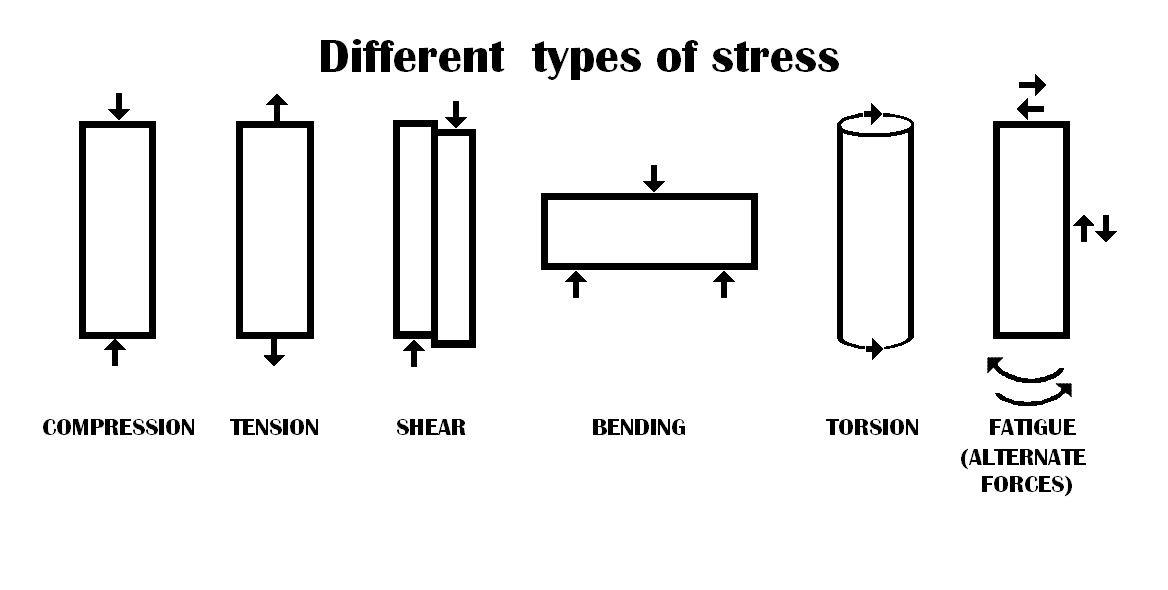
\includegraphics[width=0.6\textwidth]
    {img/DIFFERENT_TYPES_OF_STRESS.png}
  }
  \caption{Different types of stress}
  \captionsetup{font={footnotesize,bf,it}}
  \caption*{src: \url{https://upload.wikimedia.org/wikipedia/commons/e/eb/DIFFERENT_TYPES_OF_STRESS.png}}	
  \label{ToS}
\end{figure}


\section{Objectives}
\begin{figure}[!t]
  \centering
 {
    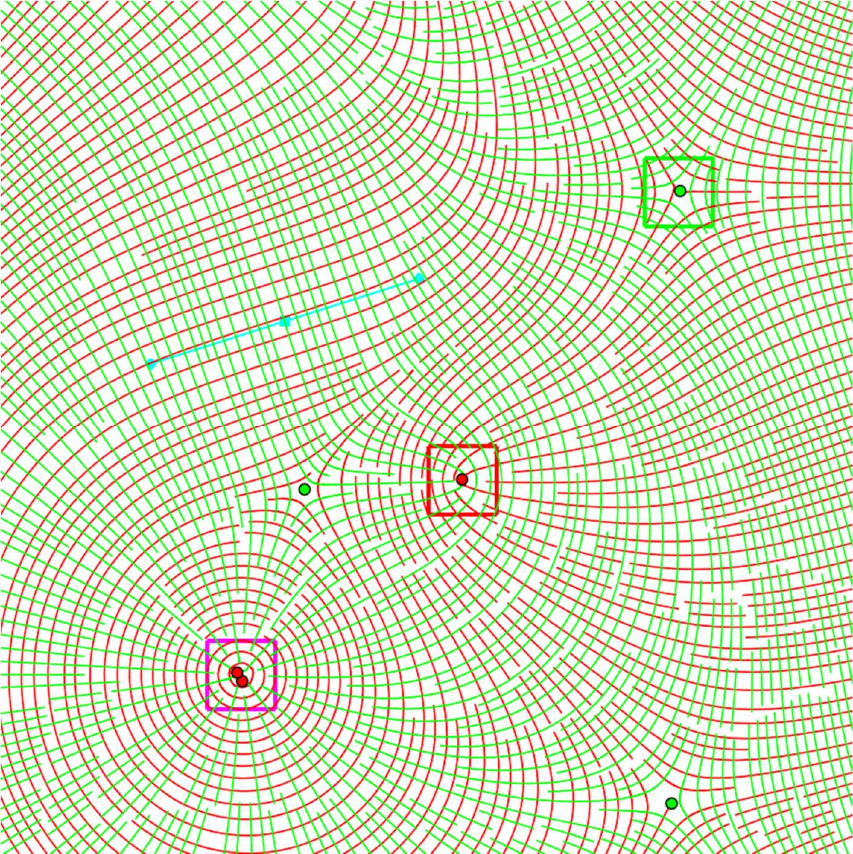
\includegraphics[width=0.5\textwidth]
    {img/hyperstreamlines.png}
  }
  \caption{Hyperstreamlines in tensor field visualization}
  \captionsetup{font={footnotesize,bf,it}}
  \caption*{src: \url{http://www2.cs.uh.edu/~chengu/Teaching/Fall2018/Lecs/Lec17.pdf}}	
  \label{streamlines}
\end{figure}
The main purpose of visualization in general, is to reduce or encode some set of numbers in some readable, explorable and more intuitive representation. This implies, e.g., clustering, structuring or projection techniques. When it comes to tensor fields, this comes in handy in, e.g., medical sciences such as in DT-MRI (diffusion tensor - medical resonance imaging) \cite{hlawatsch}, when measuring water molecule diffusion characteristics within tissue or in simulated (or measured) stress tensor fields from solid and fluid mechanics. In these named domains of science the problem arises, that tensor fields can be generated (simulated) or measured with physical/mathematical background, but not be regarded intuitively. Necessity begets ingenuity as always, which lets visualization methods and systems emerge in this context. Concurrently, the problem setting of this work encomprises the visualization of tensor fields, i.e., mostly 2D/3D-grids, commonly consisting of second-order tensors (cf. Cauchy stress tensor). In general, these grids span a spatial domain with sample positions indicated by vertices or cell centers in the dual grid, depending on the mode of interpretation. Tensor fields feature a sampling grid, consistent of tensors, which is spaced uniformly in the commonly used regular grid. A Cartesian grid, which we will utilize in this context, is a grid normalized to a certain unit length, as a special case of a regular grid. That is, each cell is formed as a unit cube in relation to the normalizing unit length. We aim to use global illumination methods to model light transport, directed by tensor fields, within such type of grids, which we consider as light propagation volumes (LPVs) \cite{dachsbacher}. Congruently, the most basic objective of this work is to design a simple light propagation scheme following the most basic but crucial physical principles and laws, like energy conservation and propagation attenuation, for tensor field visualization. Of course, the propagation scheme will need some kind of stimulus which can be defined through symbolic functions (, e.g., $r(\omega)=1$) by the user which we sample (discretize) as a primary step. This way, the approach will operate as a light transport visualization technique for light distributions given in polar coordinates, provided the user set an initial profile into the grid. Furthermore, this propagation scheme should either be used to visualize the light transport paths, defined by the anisotropy characteristics of tensor fields and tensor magnitudes of a given tensor field in a $2D$ grid. Or, as a secondary purpose, be used to visualize the light transport in a defined, given geometrical scene in a $2D$ grid. However, the tensor field needs to be preprocessed somehow to generate a footprint map of transmission profiles defined by the tensor field defined by the tensor field's anisotropy characteristics, which we will handle through matrix decompositions. For this purpose, we will let the transmission profiles act on our simple light propagation scheme to have a kind of tensor controlled directive effect on the light transport. The transmission profiles should modulate the outgoing intensities in a sense of redirection or more appropriately, redistribution. This will yield an approach, capable of computing approximated final light distributions for a given light source configuration inside of a $2D$ lattice. As this process requires a lot of user-interaction and is not to be concerned as generalizing to all possible scenarios. In the sense of automization and optimzation, another consequent aim is to implement an approach borrowed from vector-field visualization to reveal structures, which are hard to grasp by ordinary methods. We construct an FTLE-related approach in tensor field visualization (both symmetric and asymmetric) for detecting ridges representing LCS (Lagrangian Coherent Structures). These structures can be classified (identified) as repelling, attracting and saddling (forming a saddle) local features, which frequently represent key structures in nature, such as moraines in glaciers or vortices in flow fields. Commonly, in vector field visualization, LCS separate regions of different flow behavior, but in our case they separate regions/subdomains of varying directional distributions (manifesting in diverging/converging tensor field lines $\rightarrow$ compressions, tensions, roations or varying tensor magnitude $\rightarrow$ volume changes) represented by tensors, as we use our tensor-controlled light transport visualization (propagation scheme) as a basis or framework to compute the FTLE field. Consequently, we propose another method to compute an FTLE-like field on tensor fields. The FTLE field responds most where tensor field lines / hyperstreamlines converge or diverge, whereas one is the same as the other because of bidirectional stress directions and since we effectively measure the finite-time Lyapunov exponent (FTLE) with both forward and backward integration time (stimulus directions, in our case), we will detect both cases. Both invented methods, will give new insights into the topology and anisotropy of tensor fields and provide new tools for the structural analysis. The greater goal of this work is therefore the encoding of a tensor field into certain abstracted representations and the interpretation of meaningful results evaluating the proposed techniques for possible uses. The designed approach could ,e.g. , be applied in medicinal sciences, engineering and physics to reveal structures which are hard to grasp through interpreting simpler and sometimes confusing glyph and tensor field line visualizations. A classical example for tensor field visualization is plotting hyperstreamlines following major/minor eigenvectors, as depicted in Fig. \ref{streamlines}, which features a degenerate point (purple), a wedge (red) and a trisector (green).


%In diesem Abschnitt sollen neben den Herausforderungen und der
%Problemstellung insbesondere die Ziele der Arbeit beschrieben werden. 
\section{Structure of this Work}
 
For the rest of this work, we will give a quick overview on the structure and outline. Next, in chap. \ref{chap:grundlagen}, we will capture important fundamentals like tensors, polar coordinates, PCA in the context of singular value decomposition (generalization of eigenvalue decomposition), FTLE and GT datasets. Also we will discuss the most relevant related work in the domain of tensor field visualization and also in the domain of global illumination (indirect illumination rendering). Subsequently, in chap. \ref{chap:main}, we will propose the main contributions and methods of this work and document the results and evaluation in chap. \ref{chap:eval}. At last, a compact summary, conclusion and outlook will be given in chap. \ref{chap:concl}.\\

%Dieser Abschnitt wird meist recht kurz gehalten und beschreibt im
%Prinzip nur den Aufbau des Rests der Arbeit. Zum Beispiel: In Kapitel
%\ref{chap:grundlagen} geben wir einen �berblick �ber die  Grundlagen
%zu der Arbeit sowie �ber verwandte Arbeiten. In Kapitel
%\ref{chap:main} stellen wir dann \ldots vor. \ldots etc.

%%%%%%%%%%%%%%%%%%%%%%%%%%%%%%%%%%%%%%%%%%%%%%%%%%%%%%%%%%%%

\chapter{Fundamentals}
\label{chap:grundlagen}

In this chapter, we will capture the prerequisites necessary to understand the contributions of this work and we will capture tensor fields, polar coordinates, PCA, FTLE, GT datasets and related work in that sense.

%Die ersten paar Abschnitte in diesem Kapitel f�hren in die Grundlagen
%zur Arbeit ein. Das k�nnen beispielsweise Grundlagen zu Netzwerken
%oder zur Informationsextraktion sein. 

\section{Tensor Fields}
\label{sec:tensors}
Now what is a tensor? A tensor is a $o$-dimensional generalization of a matrix as illustrated in Table \ref{tensor}.
\begin{table}[!b]
\centering
\caption{Tensor Shapes}
 \begin{tabular}{c|c|c|c|c|c|c}
\textbf{order} & 0 & 1 & 2 & 3 & ... & o \\ 
\hline 
\textbf{shape} & scalar & vector & matrix & ``3D matrix'' & ... & $\mathop{o}$D matrix\\ 
\end{tabular}
\label{tensor}
 \end{table} 
In addition to that, a tensor has as many indices as its order $o$ and their run length is as long as its embedded dimension $n$ in space (the dimension of the row and column vectors), which is equal to the rank of the tensor for full rank (in other words the number of column elements n for a $n{\times}n$-matrix). A tensor is considered non-degenerate if all eigenvalues $\lambda_i>\lambda_{i+1}$ manifesting in significant anisotropy. Tensors follow certain transformation rules which are defined for covariant/contravariant tensors, which indicate the change characteristics under a basis change. Contravariant tensors do not change under a change of basis, whereas covariant tensors are not invariant w.r.t. basis changes. Tensors are most commonly obtained and defined from mathematical transformation equations. Hence, any $oD$ number array could be a tensor, but the definition holds only if the transformation rules apply to these $oD$ number arrays (in a sense of mathematical/formal interpretation). This is mostly true for component indexed $oD$ number arrays following matrix multiplication and transformation rules found in physics and math manifesting in calculation rules like matrix multiplication. Thus, a tensor in general is a $o$D number array arranged in meaningful (transformation) order, to put it simple. In fact, tensors themselves are interpreted as transformations which reflect an incoming direction vector (measuring, e.g., the stress in that direction) to an outgoing (stress) vector. To be a bit more concrete, tensors represent stress distributions in solids and fluids describing strain and flow features as these entities are not simple numbers or vectors. They occur in form of a tensors, and thus as entities or quantities in physics. That is, at each point (typically a Euclidean space or manifold) in space (indexed by the grid) there is a whole distribution of directions, e.g., stresses (elastic and viscous), which needs to be characterized and represented by a single tensor each. Collectively, defined at each point in space, these tensors form a tensor field.
\paragraph{stress tensor}
\begin{figure}[!t]
  \centering
 {
    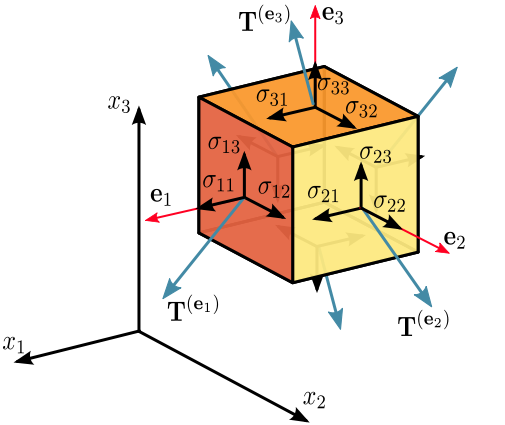
\includegraphics[width=0.6\textwidth]
    {img/stress_tensor.png}
  }
  \caption{Cauchy stress Tensor}
  \captionsetup{font={footnotesize,bf,it}}
  \caption*{src: \url{https://en.wikipedia.org/wiki/Cauchy_stress_tensor\#/media/File:Components_stress_tensor_cartesian.svg}}
  \label{cauchy}
\end{figure}

The Cauchy stress tensor, which is propably the classical example of a tensor, is depicted in Fig. \ref{cauchy} and consists of 3 stress vectors $\mathbf{T(e_i)}$, arranged in row-major order. It appears in similar form as viscous stress tensor in fluid mechanics:
\begin{align*}
\boldsymbol{\sigma}
 = \left[{\begin{matrix} \mathbf{T}^{(\mathbf{e}_1)} \\
\boldsymbol{T}^{(\mathbf{e}_2)} \\
\boldsymbol{T}^{(\mathbf{e}_3)} \\
\end{matrix}}\right] =
\left[{\begin{matrix}
\sigma _{xx} & \sigma _{xy} & \sigma _{xz} \\
\sigma _{yx} & \sigma _{yy} & \sigma _{yz} \\
\sigma _{zx} & \sigma _{zy} & \sigma _{zz} \\
\end{matrix}}\right]  = \left[{\begin{matrix}
\sigma _x & \tau _{xy} & \tau _{xz} \\
\tau _{yx} & \sigma _y & \tau _{yz} \\
\tau _{zx} & \tau _{zy} & \sigma _z \\
\end{matrix}}\right] =
\begin{bmatrix}
\sigma _{11} & \sigma _{12} & \sigma _{13} \\
\sigma _{21} & \sigma _{22} & \sigma _{23} \\
\sigma _{31} & \sigma _{32} & \sigma _{33} 
\end{bmatrix}.
\end{align*}
These 3 stress vectors represent the orientation and magnitude of total resulting stress at plane ${x,y,z}$ in plane normal directions ${x,y,z}$ ($3^2=9$ individual numbers). Thus, the stress tensor poses a full valid represenation of the stress distribution at any point in space. The stress tensor itself can be interpreted as a transformation, which maps an incoming normal direction vector $\mathbf{n}$ a resulting stress vector $\mathbf{T^{(n)}} = \mathbf{n}\cdot\boldsymbol{\sigma}$. The stresses in normal directions (diagonal elements) are directly related to the pressure, which is always isotropic and hence non-directionally dependent (kind of a Euclidean distance of the stress components). The tensor itself is a complicated representation and needs to be projected onto its principal axes to lower its dimensionality, as it is the case for principal component analysis. It is possible to find $2$ principal stress directions in $2D$ through PCA (see sect. \ref{sec:pca} below), for which there are no shear stresses existent in equilibrium. These form the principal directions of deformation at a certain location and are sufficient to describe the resulting transformation/deformation behaviour. The resulting system of principal directions and absolute stresses is often called an ``eigensystem'' or ``eigenframe''. So to say, an eigensystem, consistent of the principal directions/axes, spans a principal ellipsoid depicted in Fig. \ref{hat} in sect. \ref{sec:pca}. Another interpretation for the principal component ellipsoid is that it is the result of the tensor transformation applied to the unit circle. It is therefore somehow representing the distortion of an absolutely isotropic object (unit circle) by whatever the underlying affine tensor transformation effects (e.g. stretching, shearing, mirroring, scaling, rotating). Let us consider it as some lower dimensional, more intuitive representation of the tensor which we were left with in the first place. To put it all together, a tensor is a mathematical transformation which is encoded inside of an abstract $oD$ number array, which comes in need, whenever we have a whole distribution of directions manifesting itself inside of a tensor (matrix) transformation.

\section{Polar Coordinates}
\label{sec:polar}
\begin{figure}[!t]
  \centering
 {
    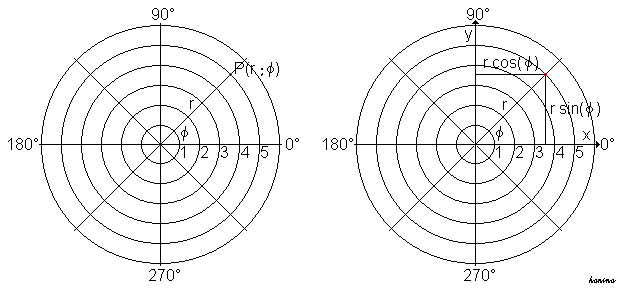
\includegraphics[width=0.8\textwidth]
    {img/polarkoordinaten.png}
  }
  \caption{polar space}
  \captionsetup{font={footnotesize,bf,it}}
   \caption*{src: \url{https://de.wikipedia.org/wiki/Datei:Ebene_polarkoordinaten.PNG}}
  \label{polar}
\end{figure}\vskip 3pt
Mathematically speaking, a polar space is a system, which maps each angle $\omega$ a magnitude $r(\omega)$ through a symbolic function. The conversion formula from polar (given a radius $r$ and angle $\omega$) to Cartesian coordinates is depicted in Fig. \ref{polar} and is given by:
\begin{align*}
	x &= r \cos \omega, \\
 	y &= r \sin \omega.
\end{align*}
Note, that we switched angle $\phi$ to $\omega$ for reasonable discrimination to the radiant intensity. The inverse direction (given coordinates $x,y$) is a bit more complicated:
\begin{align*}
	r &= \sqrt{x^2 + y^2} \\
\omega &= \operatorname{atan2}(y, x)
\end{align*}
The polar domain is a circular axis version of the domain $[0..2\pi]$, with negative magnitudes in $r$ shifted by 180 degrees (point reflected) as this is the formal behaviour defined and required by the conversion formulas.

\section{Principal Component Analysis}
\label{sec:pca}
Note, that we denote a matrix with a second order tensor interchangeably for the sake of simplicity in the following. Also keep in mind, that we interpret a matrix or tensor as affine transformation. For any state of stress in equilibrium it is possible to find $n$ (dimensionality) independent orthogonal directions with no shear stresses existent. Along these directions the principal stresses, which are normal (tensile/compressive) stresses, are exerted. The anisotropy can be represented by, e.g., ellipsoid glyphs.

\begin{figure}[!t]
\hskip 22pt
  \begin{minipage}[!t]{0.4\textwidth}
    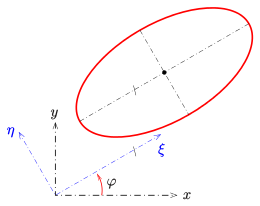
\includegraphics[width=\textwidth]{img/HAT.png}
   \caption{2D principal component ellipsoid\/ glyph (eigenframe)}
   \label{hat}
   \captionsetup{font={footnotesize,bf,it}}
   \caption*{src: \url{https://de.wikipedia.org/wiki/Datei:HAT-ellipse0.svg}}
  \end{minipage} \hskip 40pt
  %\raggedright
  \begin{minipage}[!t]{0.4\textwidth}
    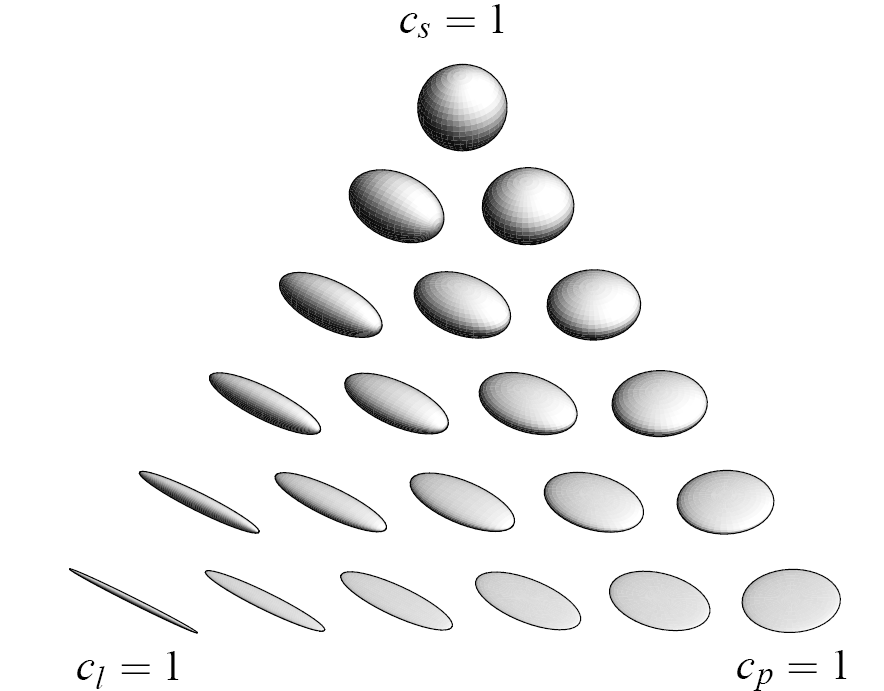
\includegraphics[width=\textwidth]{img/glyphs.png}
    \caption{3D ellipsoid glyphs w. anisotropy coefficient (l:linear, p:planar, s:spherical)}
    \label{3Dglyphs}
    \captionsetup{font={footnotesize,bf,it}}
   \caption*{src: \url{https://slideplayer.com/slide/5291764/}}
  \end{minipage}
\end{figure}

Principal Component Analysis is an algorithm, which is able to capture the principal components (directions) in stochastic data. But it works similarly on transformations to capture the principal directions from transformations like rotation and scaling. Now, principal component analysis can be done by eigenvalue or singular vector decomposition, whereas the former yields complex eigenvalues for asymmetric matrices. For (skew-) symmetric (normal) matrices, they are connected through the following relation: $s_i = \sqrt{|\lambda_i|}$ (cf. \cite{kieburg}). Note, that the eigenvectors match the singular vectors only for symmetric matrices, which does not mean that they do not form the half-axes of the principal component ellipsoid in other cases (cf. \cite{moler}). Mathematically speaking, a decomposition is somehow decomposing a transformation (which follows certain transformation rules) into parts of subsequent transformations consistent of rotation and scaling (classically: $\mathbf{A} = \mathbf{R}\mathbf{S}\mathbf{R}^*$). We choose to use singular value decomposition ($\mathbf{A} = \mathbf{U} \mathbf{\Sigma} \mathbf{V}^*$) to be able to set up real eigenvalues for any kind of matrix (singular values are always real and positive). Also, the singular vectors of the $\mathbf{U}$-matrix represent the half-axes of the principal ellipsoid (eigenframe) shown in Fig. \ref{HAT} for any kind of transformation matrix. The singular value decomposition is defined as follows:
\begin{align*}
	\mathbf{A} = \mathbf{U} \boldsymbol{\Sigma} \mathbf{V}
\end{align*}
where
\begin{itemize}
	\item $\mathbf{U}$ is an $m � m$ unitary matrix
	\item $\boldsymbol{\Sigma}$ is a diagonal matrix {$m � n$} with positive real numbers on the diagonal
	\item $\mathbf{V}$ is an {$n � n$} unitary matrix, $\mathbf{V}^*$ is its conjugate transpose
\end{itemize}
 
In addition, we also calculate the eigenvalues to exploit the sign of the real part of the eigenvalues (\cite{mroz}) ordered decreasingly by absolute value (corresponding to singular value order). The sign corresponds to tensile ($+$) and compressive ($-$) stress, which would allow us to visualize deformation glyphs with arrows pointing inwards for compressive and outwards for tensile stresses. We do this decomposition analysis once for each matrix and then store the precomputed results in a grid. The principal ellipsoid is also used as a transmission profile for the propagation scheme in symbolic form in a subequent step, which makes it a basic and central concept within the scope of this work. Within this work, we will use the singular vectors yielded from singular value decomposition to avoid complex values yielded from eigenvalue decomposition. This will allow us to set up glyphs representing the major/minor axis of the underlying transformation for every kind of (asymmetric/symmetric) tensor. We will then use global-illumination techniques on top to generate a light transport flow map, which permits us somehow to forward the intensities which are given as predefined initialization values in form of symbolic functions defined by the user. This kind of light transport propagation scheme will also allow us to compute an FTLE-like field on the tensor fields.

\section{Finite-Time Lyapunov Exponent}
\label{sec:ftle}
The Finite-Time Lyapunov Exponent is a measure, developed to analyze time-dependent dynamical systems for their separation abilities concerning massless tracer particles. We imagine a flow field, i.e., a vector field which in turn represents the effective amount or concentration shifted into a particular direction at each point in space. It could induced by e.g. concentration or height gradients. This flow field is considered a time-dependent dynamical system, since it usually holds a time-component $t$ and thus maps each initial position an aged (altered) position: $\mathbf{\upvarphi}(\mathbf{x}) : \mathbf{x}(t_0) \longmapsto \mathbf{x}(t_0+T)$. We can now imagine placing two close by particles in distance $\delta$ into a flow field and run a time dependent simulation. Remark that this corresponds to the Lagrangian view in vector fields, which travels with the particles (instead of taking the position of a resting observer - Eulerian view):

\begin{figure}[!t]
  \centering
 {
    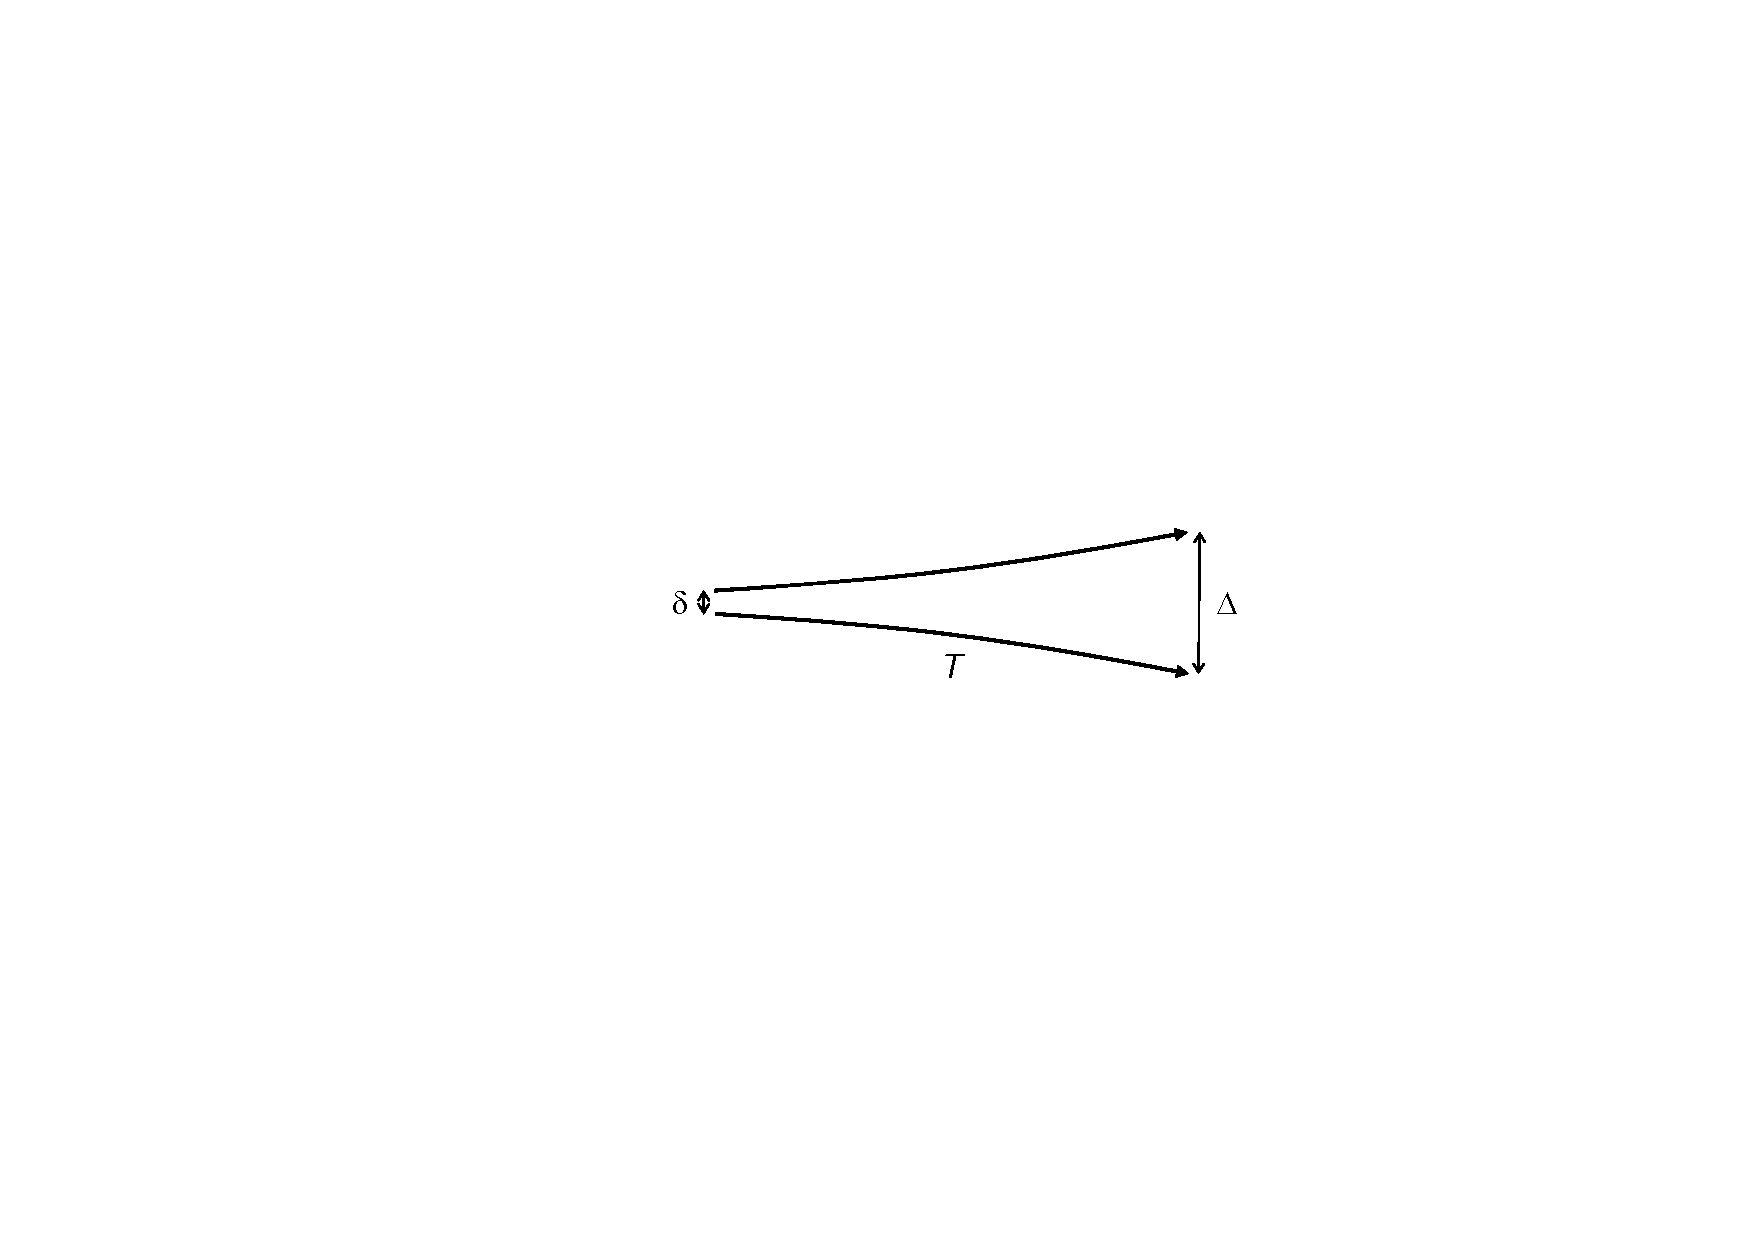
\includegraphics[width=0.6\textwidth]
    {img/ftle_sep.pdf}
  }
  \caption{FTLE: separation of massless tracer particles}
  \captionsetup{font={footnotesize,bf,it}}
  \caption*{src: Skript Prof. Sadlo, Scientific Visualization SS2017, Heidelberg University}
  \label{ftle_sep}
\end{figure}

We observe particle trajectories diverging w.r.t. the central axis ending up in distance $\Delta$. The FTLE measure for this single example (point in space) is then defined as:

\begin{align*}
	\sigma = \frac{1}{\lvert T\rvert}\ln \frac{\Delta}{\delta}
\end{align*}

Alternatively, an FTLE can also be computed from a flow map's gradient, which is more convenient to compute in general:
\begin{align*}
	\sigma(\mathbf{x})=\frac{1}{\lvert T\rvert}\ln \lvert\lvert\nabla\mathbf{\upvarphi(x)}\rvert\rvert _2,
\end{align*}
whereas $\lvert\lvert A\rvert\rvert _2 = \sqrt{\lambda_{max}(A^TA)}$ is the spectral norm of matrix $A$. This will yield a map, which responds most where path lines diverge w.r.t. to a central axis. We consider an example which detects FTLE ridges inside of the cross-section of a double gyre. Note, that this example considers single trajectories diverging implicitly:
\begin{figure}[!t]
\hskip 22pt
  \begin{minipage}[!t]{0.4\textwidth}
    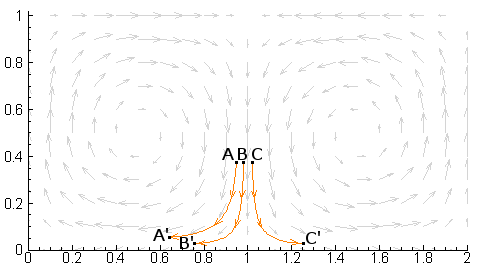
\includegraphics[width=\textwidth]{img/diverge.png}
   \caption{diverging streamlines for double gyre}
   \label{diverge}
   \captionsetup{font={footnotesize,bf,it}}
   \caption*{src: \url{https://shaddenlab.berkeley.edu/uploads/LCS-tutorial/dg_3traj.png}}
  \end{minipage} \hskip 40pt
  %\raggedright
  \begin{minipage}[!t]{0.4\textwidth}
    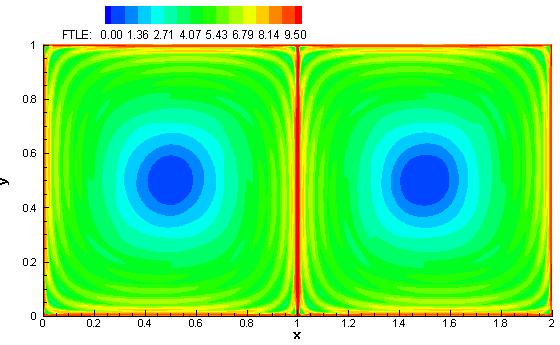
\includegraphics[width=\textwidth]{img/ftle_gyre.png}
    \caption{FTLE field for double gyre}
    \label{ftle_gyre}
    \captionsetup{font={footnotesize,bf,it}}
   \caption*{src: \url{https://shaddenlab.berkeley.edu/uploads/LCS-tutorial/dle_incT.png}}
  \end{minipage}
\end{figure}
Fig \ref{diverge} and \ref{ftle_gyre} depict a scenario of diverging streamlines for a double gyre snapshot in time (yielding a time-independent dynamical system). Fig. \ref{ftle_gyre} features a high ridge on the margins (borders) and in particular at the center of the domain. This region of interest (ROI) is considered to indicate the maximum relative local divergence of tensor field lines, by the approach. Ridges also represent Lagrangian Coherent Structures, which are found in nature in vortices of correlating flow behavior.  We could imagine to introduce this process for a whole distribution of trajectories, which would implement an FTLE for uncertain vector fields in a sense, that whole propability distributions of trajectories could be heeded. An overview about existing visualization techniques for uncertain data is given by Griete \& Schuhmann \cite{griete}. We require that the trajectories can cross each other unaffectedly, i.e., the superposition principle is supposed to be respected for the magnitudes. But behold, is this behavior not somehow familiar? If we elaborately think this through, we can come up with the idea that this is the behavior of light propagation in vacuum. Light paths are physically allowed to cross each other with no influence exerted on each other at all. Consequently, we choose to model the distributions of trajectories as light intensity profiles. That is, we interpret the polar profiles as a propability density function (PDF) for particle trajectories heading into this direction. To put it into context, our main contribution method LTG uses the FTLE as an inspiration or template to design a similar approach for tensor field visualization. The main difference to the template FTLE is that we follow eigenvectors instead of flow vectors and that we use whole distributions of trajectories, as a tensor field suggests whole distributions of directions, accordingly.

\section{GT Datasets / Methods}
\label{sec:gt}
\paragraph{Glyphs and Tensor Field Lines}
%\begin{figure}[!t]
%  \centering
% {
%    \includegraphics[width=0.4\textwidth]
%    {img/tensorfieldlines.png}
%  }
%  \caption{tensor field lines: bold lines; ellipsoids: ellipsoid glyphs}
%  \label{scheme}
%\end{figure}
Glyphs are derived as a basis for the weighting profiles of the tensors in the following propagation scheme. They were chosen because it is an easy-to-use (understand) concept, which can also be interpreted nicely. In fact, these representations are used for the principal component analysis of direction vectors for the tensor field line extrapolation (integration) and also as transmission profiles for the light propagation scheme in a subsequent step. We can again emphasize glyphs as a crucial, central concept within this work. Tensor field lines (the type of tensor streamline analog that does not introduce artificial intertia) were implemented for ground truth (GT) data generation purposes. For example, when designing a FTLE-like field computation technique, we will need to know when tensor field lines diverge/converge. Examples for glyphs (ellipsoids) and tensor field lines (thin lines) are depicted in Fig. \ref{test-fields}.

\paragraph{Test Data (Generation)}
We used python's numpy library to generate predefined, synthetic test cases and caught two real data example from \url{TensorVis.org} and \url{https://www.cs.purdue.edu/homes/cs530/projects/project5.html}, which needed to be pre-processed through slicing and subsequent cropping to obtain $2D$ samples ($2\times2$) matrices). These test fields can be grouped into symmetric and asymmetric ones:\\

\begin{figure}[!t]
\centering
  \begin{minipage}{0.3\textwidth}
    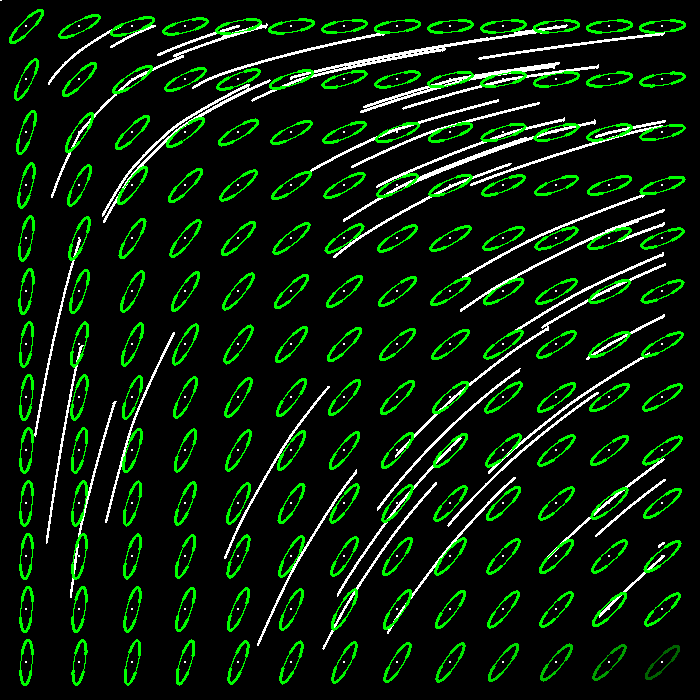
\includegraphics[height=\textwidth]{img/corner-TFL.png}
    \caption*{``corner''}
    \label{a)}
  \end{minipage}
  \begin{minipage}{0.3\textwidth}
    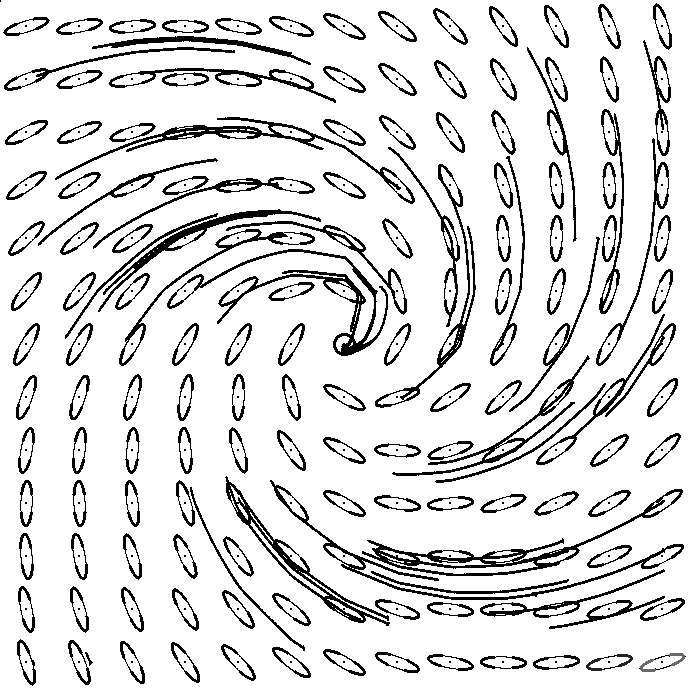
\includegraphics[height=\textwidth]{img/spiral-TFL.png}
    \caption*{``spiral''}
    \label{b)}
  \end{minipage}
  \begin{minipage}{0.3\textwidth}
    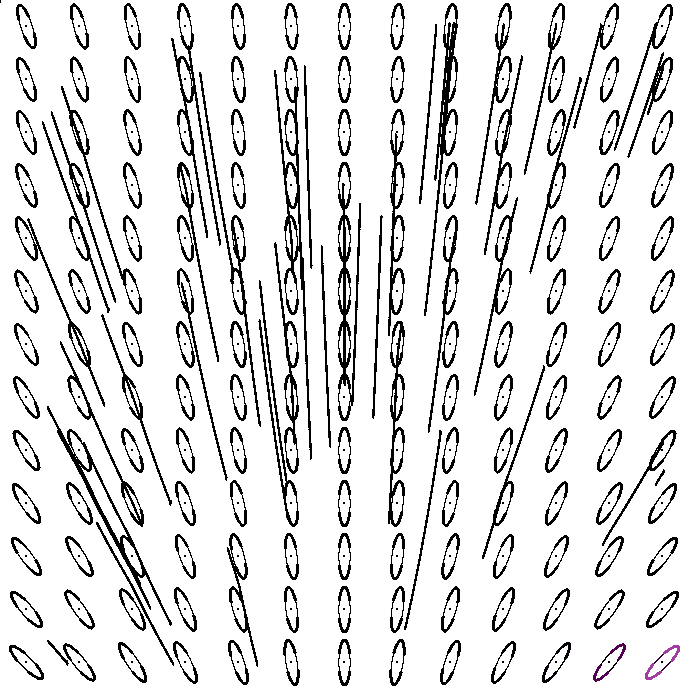
\includegraphics[height=\textwidth]{img/drain_old.png}
    \caption*{``V''}
    \label{b)}
  \end{minipage}
\caption{Named test fields}
\label{test-fields}
\end{figure}

\textbf{Asymmetric Tensor Fields}

\begin{figure}[!t]
\centering
  \begin{minipage}{0.4\textwidth}
  \centering
    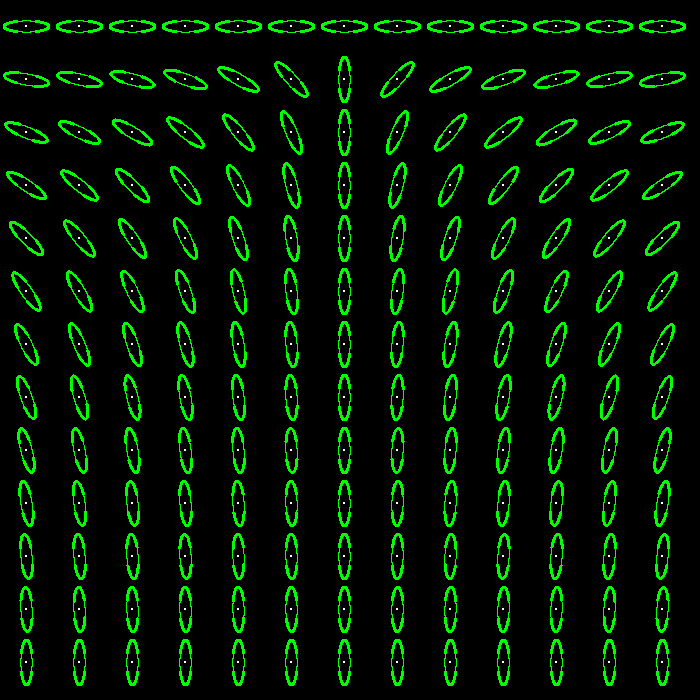
\includegraphics[width=0.8\textwidth]{img/drain(alt).png}
    \caption*{a) glyphs}
    \label{a)}
  \end{minipage}
  \begin{minipage}{0.4\textwidth}
    \centering
    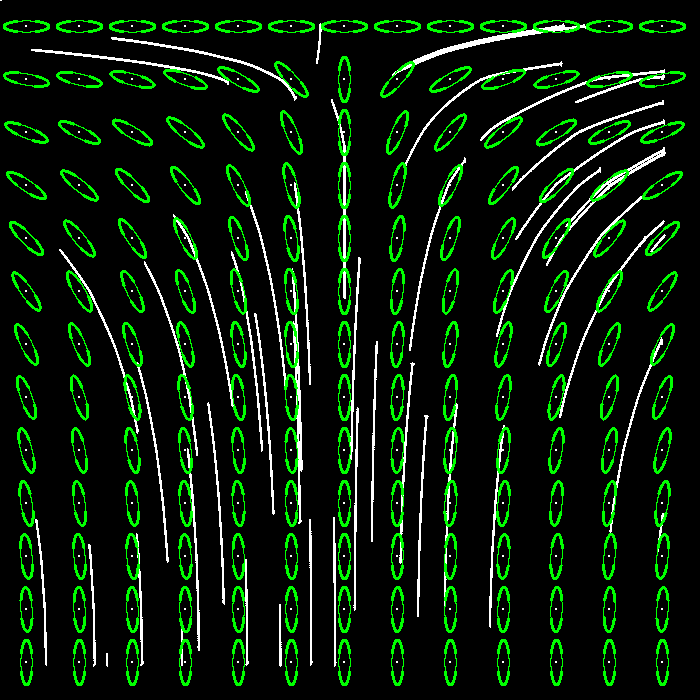
\includegraphics[width=0.8\textwidth]{img/drain(alt)-TFL.png}
    \caption*{b) tensor field lines for a)}
    \label{b)}
  \end{minipage}
\caption{``drain'' test field}
\label{drain}
\end{figure}

The ``drain''-Testfield, depicted in Fig. \ref{drain} is generated to have a kind of proof-of-concept (POC) for the FTLE-related approach. It poses raw, bare diverging tensor field lines without any other feature modulated on top. Thus, it can be expected to induce a high FTLE response, since it is an interpretable ground truth test and is considered to be a basic trigger/stimulus for the approach with no side effects introduced.

\begin{figure}[!t]
\centering
  \begin{minipage}{0.4\textwidth}
  \centering
    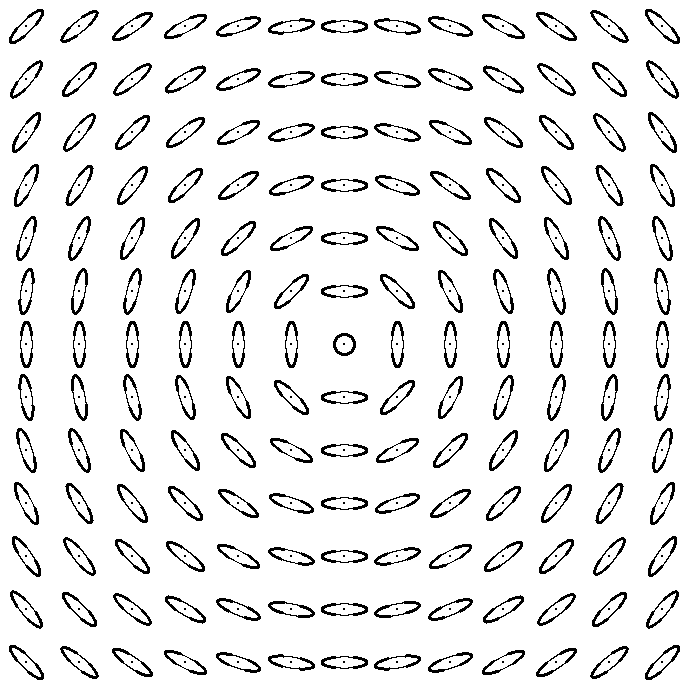
\includegraphics[width=0.8\textwidth]{img/rings.png}
    \caption*{a) glyphs}
    \label{a)}
  \end{minipage}
  \begin{minipage}{0.4\textwidth}
   \centering
    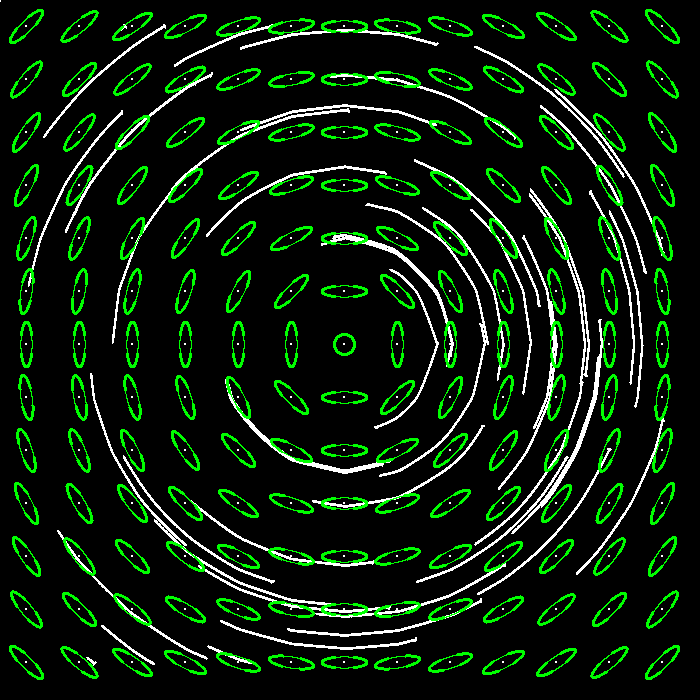
\includegraphics[width=0.8\textwidth]{img/tensorfieldlines.png}
	\caption*{b) tensor field lines for a)}
    \label{b)}
  \end{minipage}
\caption{``rings'' test field}
\label{rings}
\end{figure}
The ``rings'' test field, depicted in Fig. \ref{rings} should be used to demonstrate the directive ability of the approach transmitting energy in circular orbits.
\begin{figure}[!t]
\centering
  \begin{minipage}{0.4\textwidth}
    \centering
    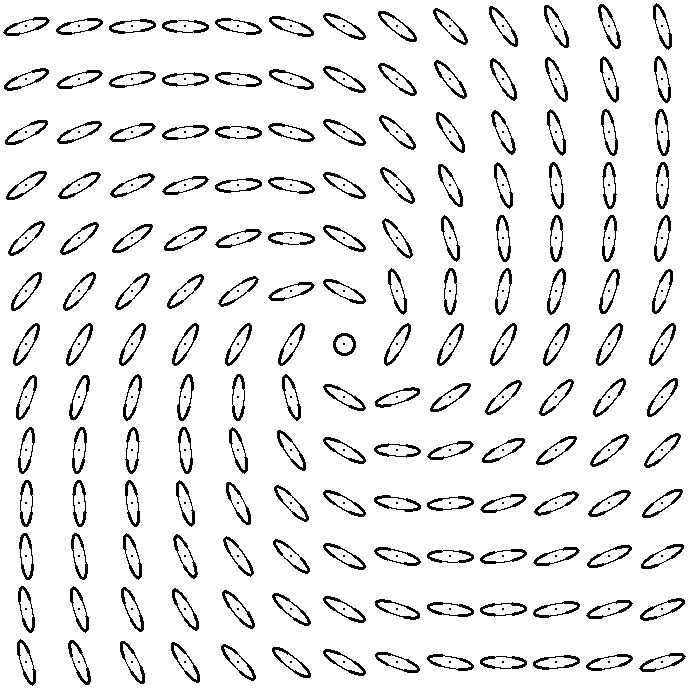
\includegraphics[width=0.8\textwidth]{img/spiral.png}
    \caption*{a) glyphs}
    \label{a)}
  \end{minipage}
  \begin{minipage}{0.4\textwidth}
    \centering
    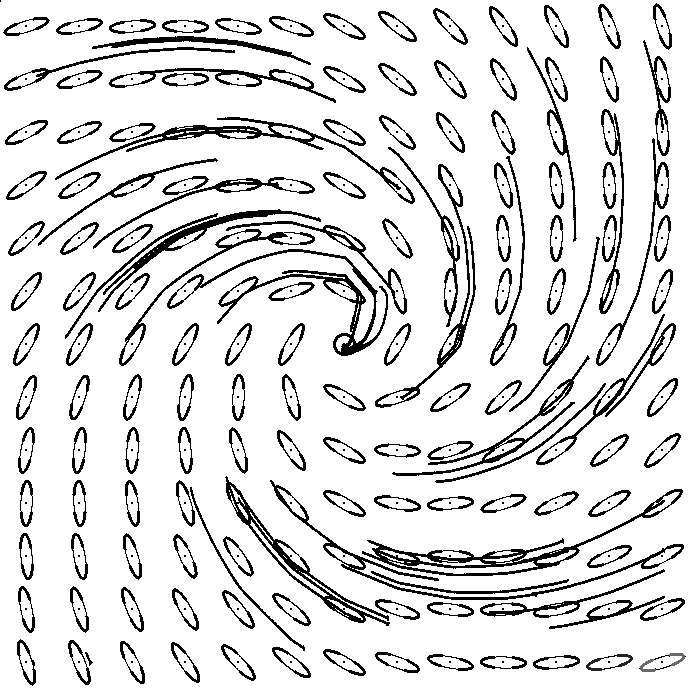
\includegraphics[width=0.8\textwidth]{img/spiral-TFL.png}
    \caption*{b) tensor field lines for a)}
    \label{b)}
  \end{minipage}
\caption{``spiral''-test field}
\label{spiral}
\end{figure}
The ``spiral'' test field, depicted in Fig. \ref{spiral} should be used to demonstrate the directive ability of the approach transmitting energy in archimedian spiral orbits.
\begin{figure}[!t]
\centering
  \begin{minipage}{0.4\textwidth}
    \centering
    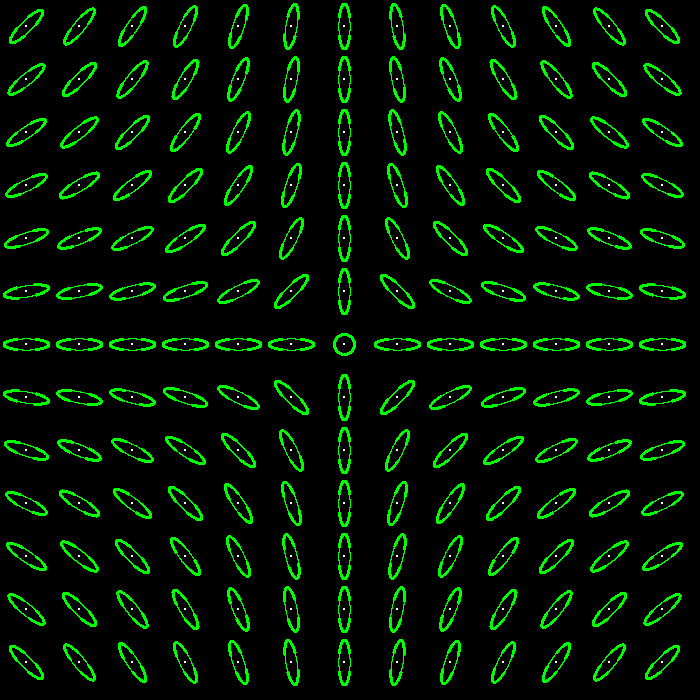
\includegraphics[width=0.8\textwidth]{img/inverse.png}
    \caption*{a) glyphs}
    \label{a)}
  \end{minipage}
  \begin{minipage}{0.4\textwidth}
    \centering
    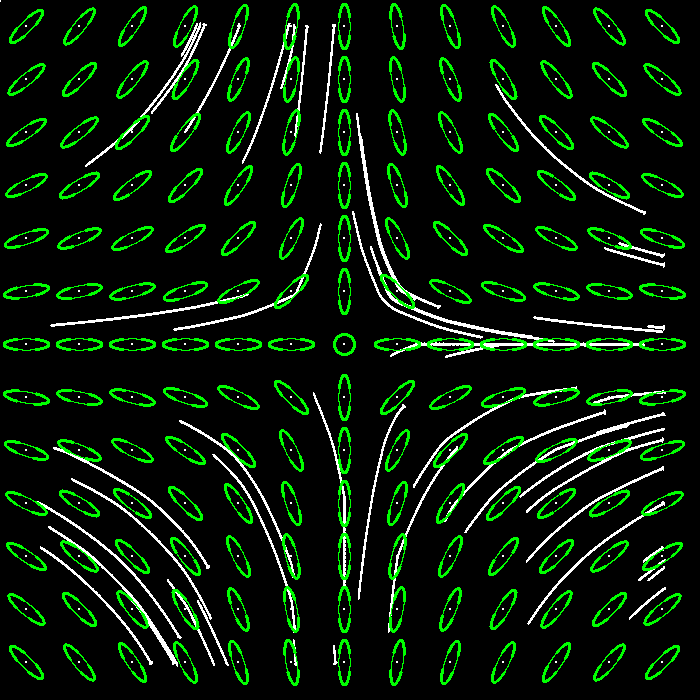
\includegraphics[width=0.8\textwidth]{img/inverse-TFL.png}
    \caption*{b) tensor field lines for a)}
    \label{b)}
  \end{minipage}
\caption{``inverse'' test field}
\label{inverse}
\end{figure}
With the \enquote{inverse} test field we want to demonstrate the directive separation of intensities into four quadrants.


\begin{figure}[!t]
\centering
  \begin{minipage}{0.4\textwidth}
    \centering
    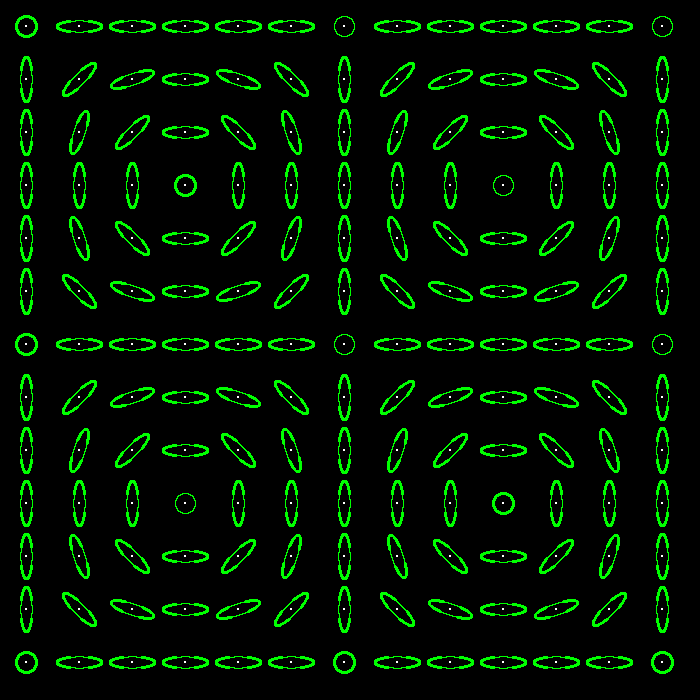
\includegraphics[width=0.8\textwidth]{img/gyre.png}
    \caption*{a) glyphs}
    \label{a)}
  \end{minipage}
  \begin{minipage}{0.4\textwidth}
    \centering
    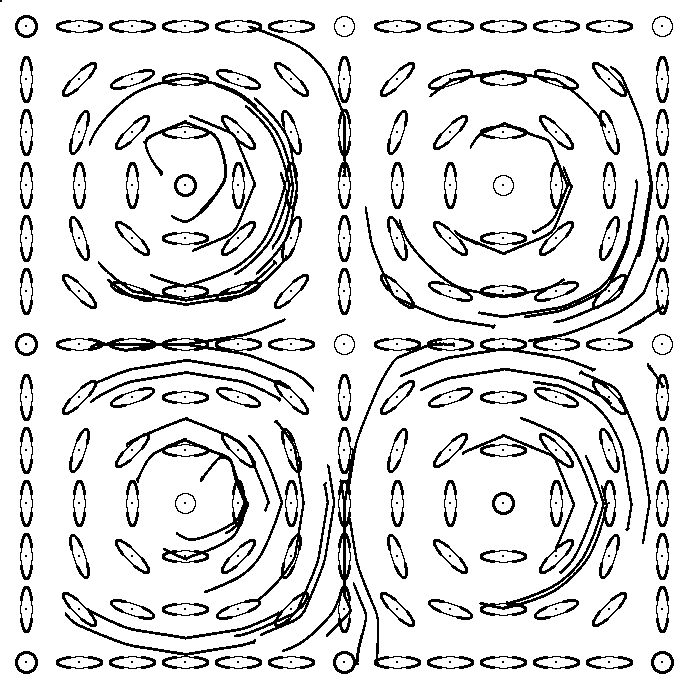
\includegraphics[width=0.8\textwidth]{img/gyre-TFL.png}
    \caption*{b) tensor field lines for a)}
    \label{b)}
  \end{minipage}
\caption{a) ``gyre''-test field, b) tensor field lines for a)}
\label{gyre}
\end{figure}
The test field ``gyre'', depicted in Fig \ref{gyre}, constitutes a sustained turn over the grid representing the redirection or forwarding along domain corners. 


\textbf{Symmteric Tensor Fields}
We also aim to use a real data example of the $3D$ DTI-MRI diffusion tensor of the brain for a male subject at the age of 27 and another one featuring a human heart. As we visualize 2D symmetric second order tensor fields, we need to slice the dataset and crop the $2{\times}2$ matrices omitting the $z$-component of the original $3{\times}3$ matrices. Fig. \ref{brainglyphs} depicts the glyph representation of the test dataset for slice index $15$. To have some real examples involved, we apply the invented technique to both DTI-MRI \enquote{brain} and \enquote{heart} scans, which can be observed in Fig. \ref{real1} and \ref{real2}.
\begin{figure}[!t]
\centering
  \begin{minipage}{0.4\textwidth}
  \centering
    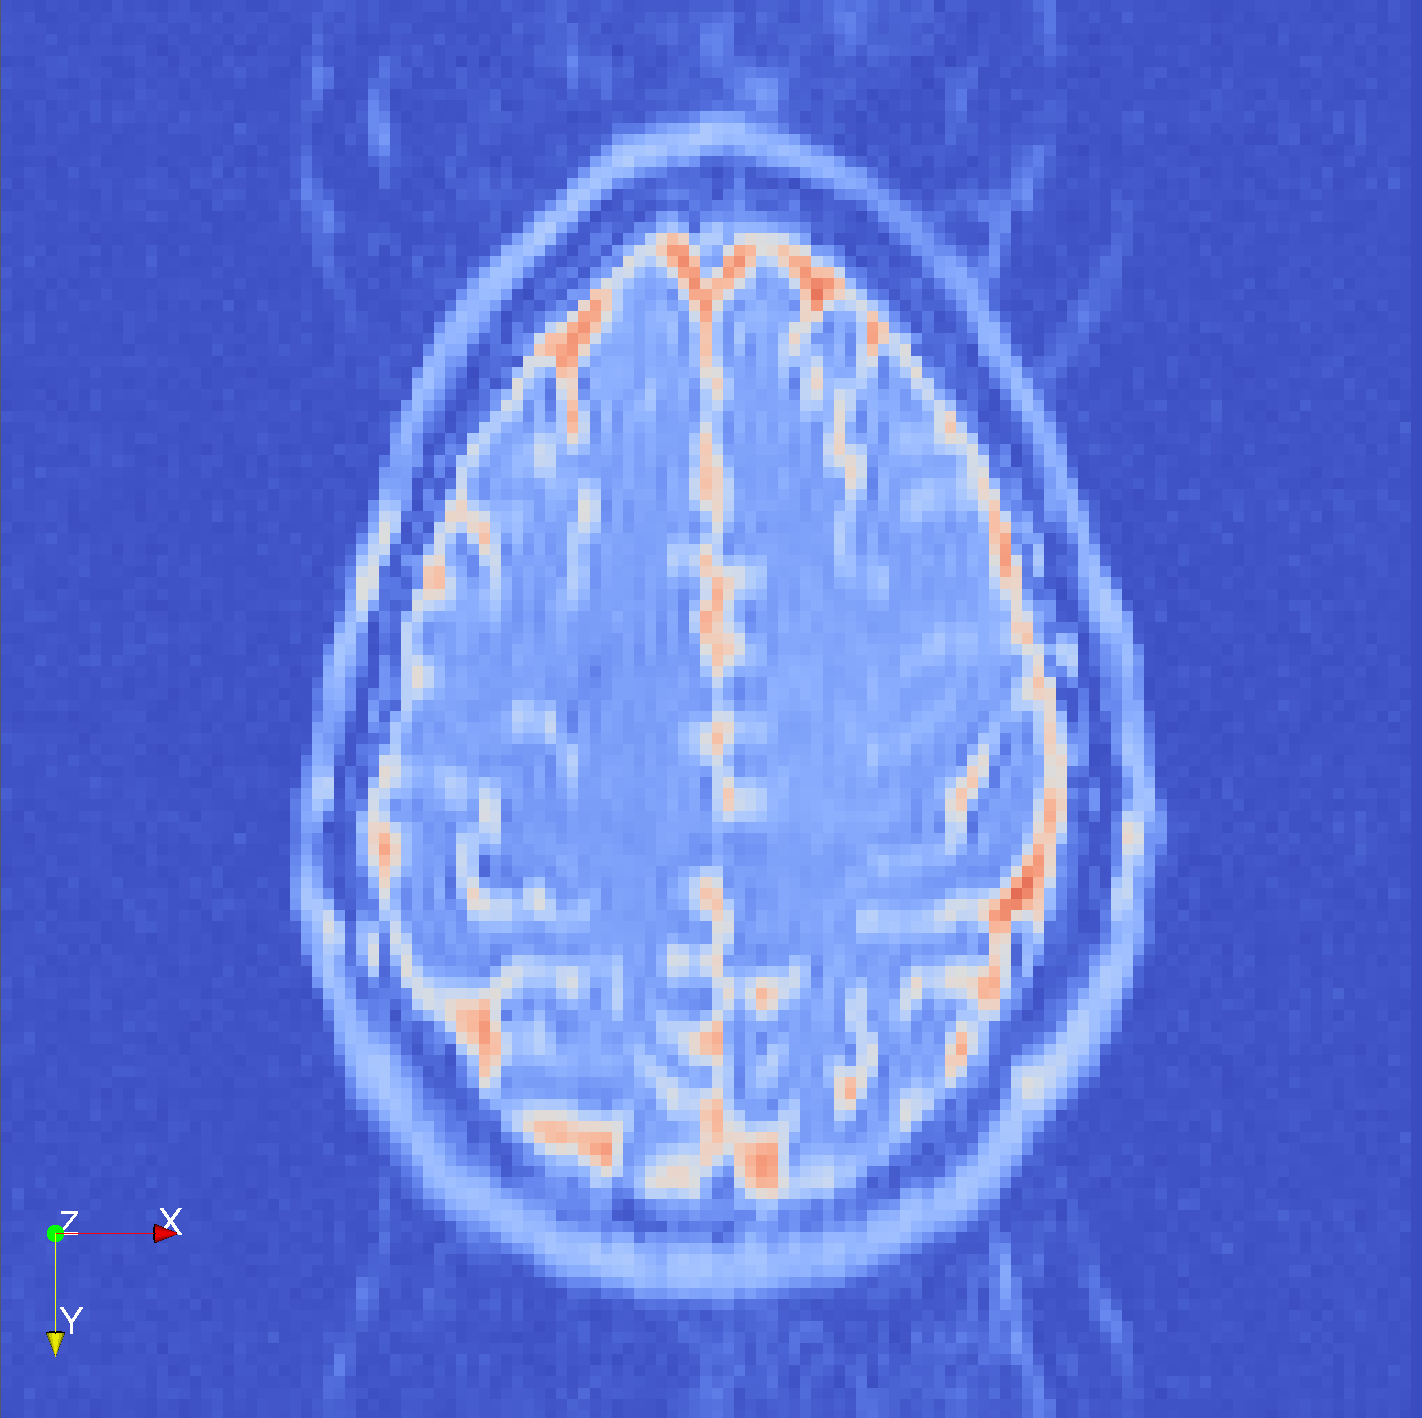
\includegraphics[width=0.8\textwidth]{img/brain_org.png}
    \label{a)}
    \caption*{tensor magnitude}
  \end{minipage}
  \begin{minipage}{0.4\textwidth}
  \centering
    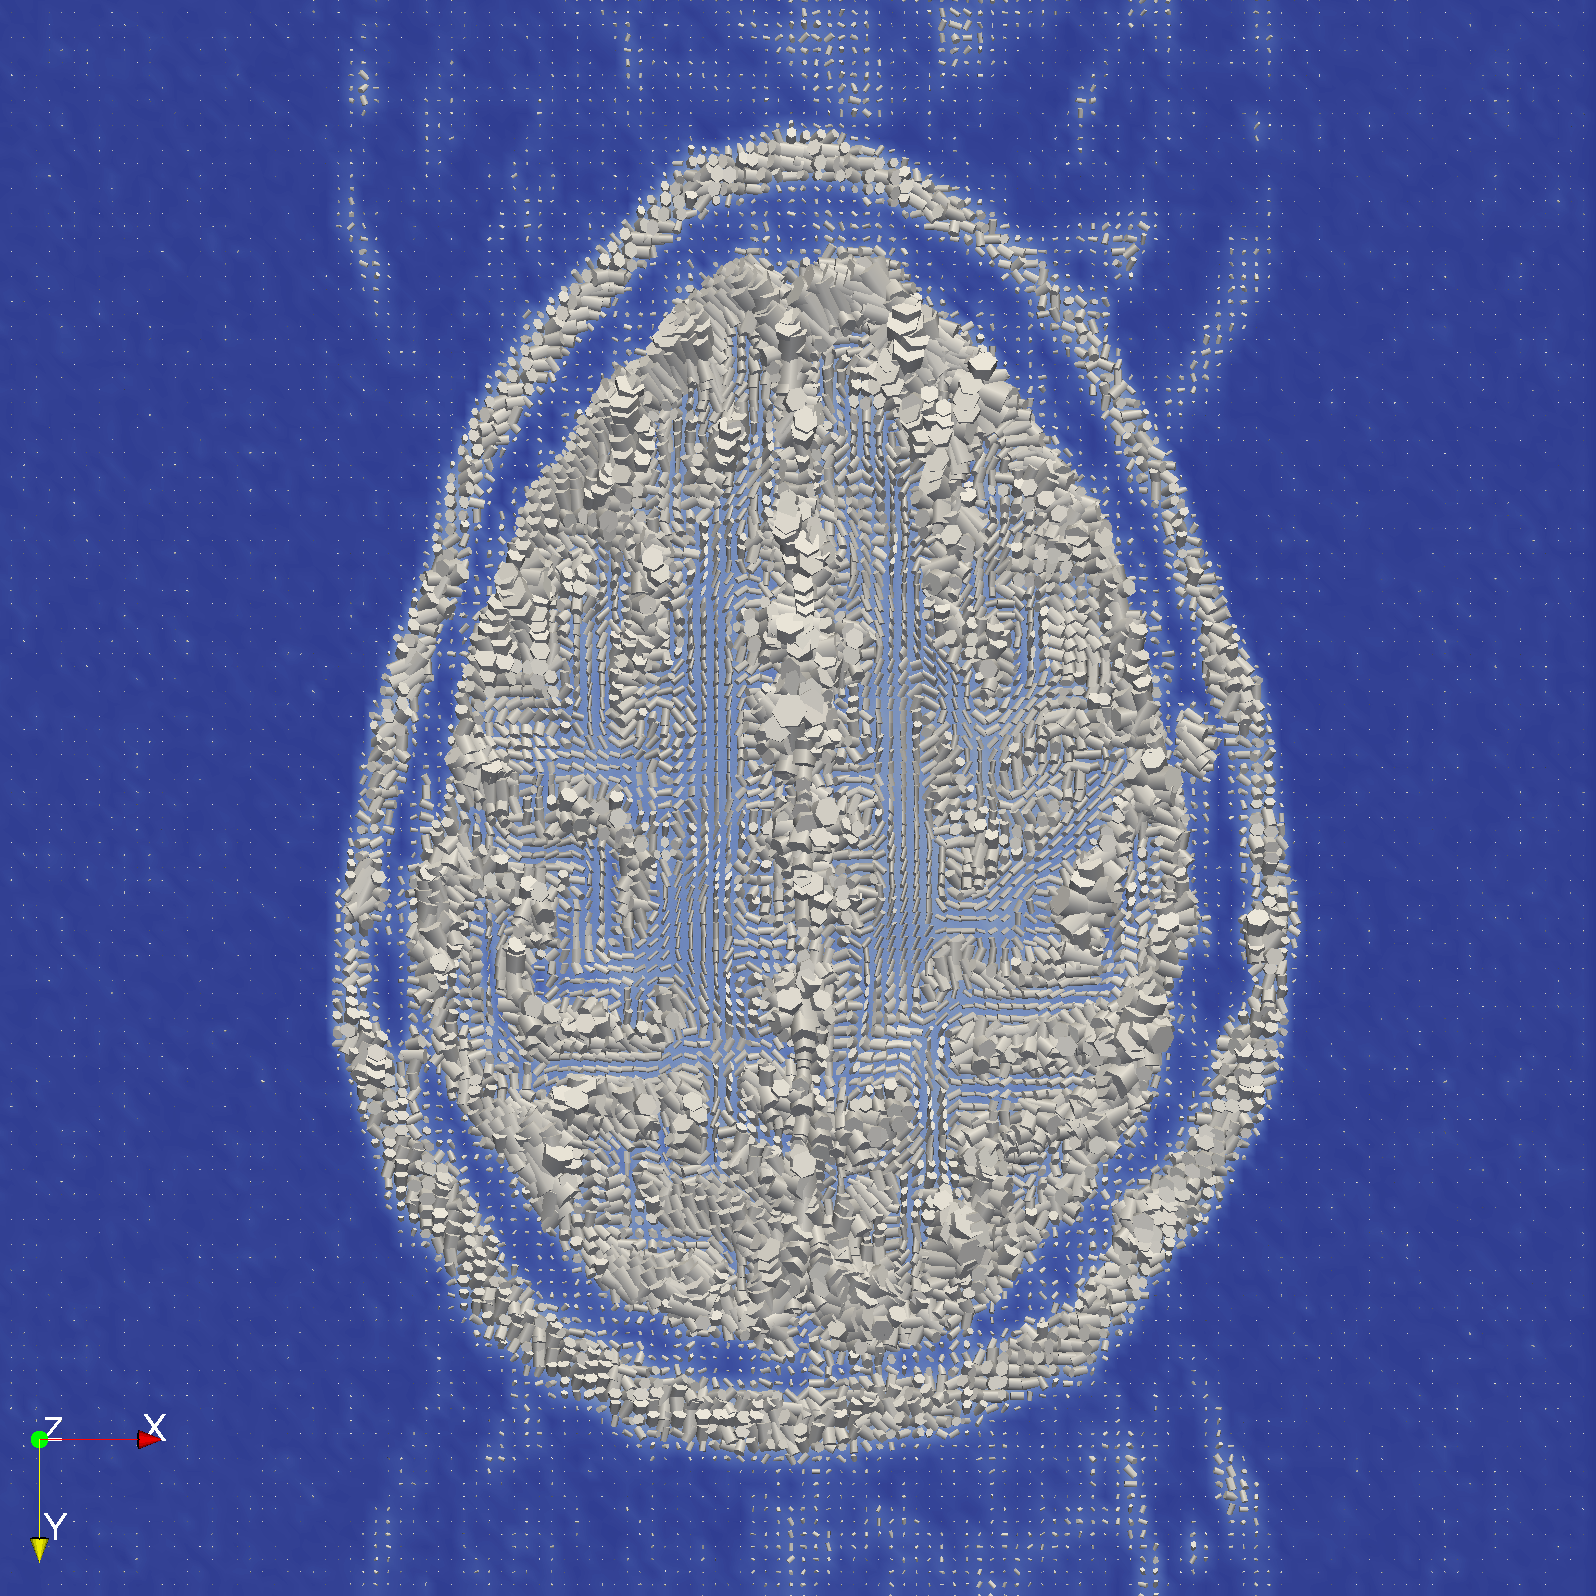
\includegraphics[width=0.8\textwidth]{img/brain_cyl_glyphs.png}
    \label{b)}
    \caption*{cyclinder glyphs}
  \end{minipage}
\caption{Real data examples: \enquote{brain} dataset}
\label{real1}
\end{figure}
Observing the \enquote{brain} dataset in Fig \ref{real1}, one may notice that it introduces a lot of variances to tensor magnitude and linear anisotropy. We choose this DTI-MRI scan as an example-par-excellence for real application data given in a reasonable resolution.
\begin{figure}[!t]
\centering
  \begin{minipage}{0.4\textwidth}
    \centering
    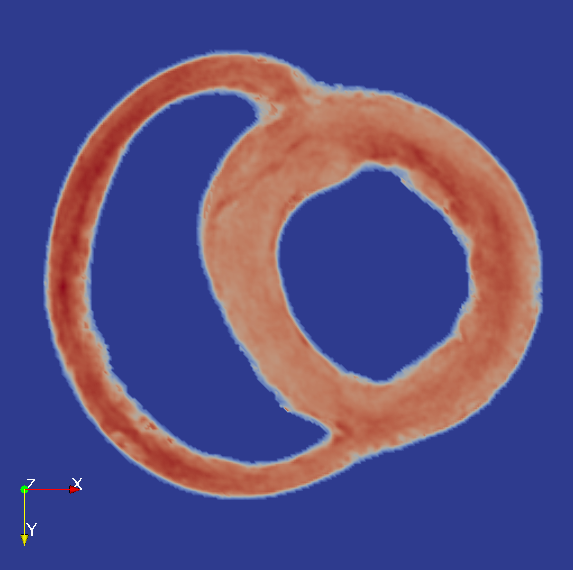
\includegraphics[width=0.8\textwidth]{img/heart_org.png}
    \label{a)}
    \caption*{tensor magnitude}
  \end{minipage}
  \begin{minipage}{0.4\textwidth}
    \centering
      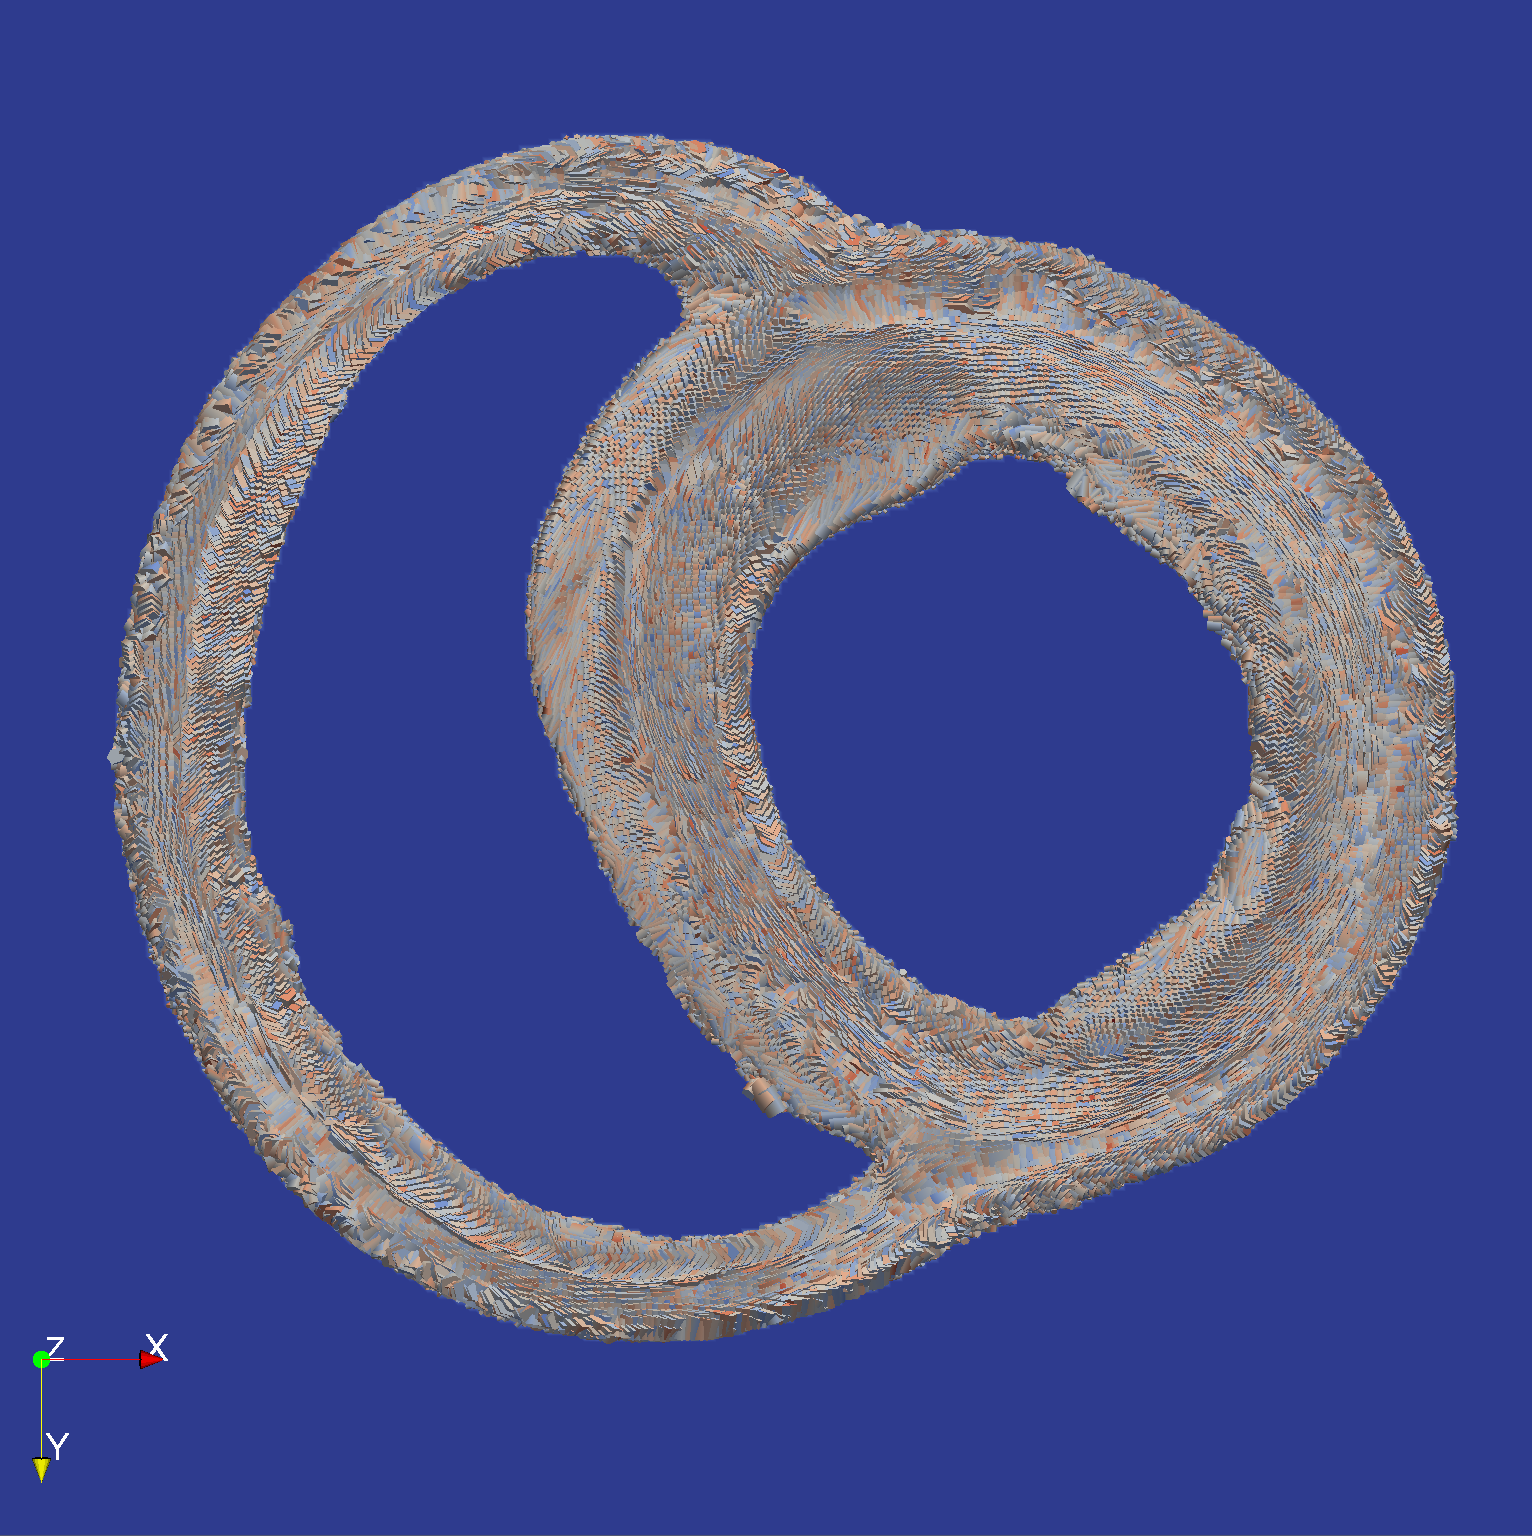
\includegraphics[width=0.8\textwidth]{img/heart_cyl_glyphs.png}
    \label{b)}
    \caption*{cyclinder glyphs}
  \end{minipage}
\caption{Real data examples \enquote{heart} dataset}
\label{real2}
\end{figure}
When we look at this DT-MRI scan of a human heart we can notice the elongated shape, which we consider to represent the aorta and a part of the rest of the heart. If we consider the glyph representation, we again infer, that we incorporate lots of anisotropic regions with varying tensor magnitudes here.


\chapter{Related Work}
\label{chap:related}

There has been extensive recent work on symmetric tensors but in comparison little on asymmetric ones. Since we are not able to cover the whole scope in this work, we will focus on the most relevant works on tensor field visualization. We will talk about the publications from Hlawatsch et al. \cite{hlawatsch} and Zirr et al. \cite{zirr} in particular, since they constitute thematically close related works. But first, we will cover related works on global illumination methods, as these form a basis or prerequisite for our work. Please note, that they do not focus on tensor field visualization at all. Remember, that we will inventively employ global illumination methods for tensor field visualization as an innovative step and that we want to cover previous works on our base approach, as well.

\paragraph{Global Illumination Methods}
Since we use a specific category of global illumination methods as a basis, we decide to only discuss lattice based methods which work, corresponding to their name, on a grid. Remark, that Global Illumination methods classically focus on realistic indirect lighting. Thus, they aim on producing a most realistic image, what in our case turns out to be a most informative image in correspondence. The most early work in this field is propably the Discrete Ordinates Method (DOM) by Chandrasekhar \cite{Chandrasekhar}, which is used specifically for computing radiative transfer in participating media (volume rendering). The radiative transfer equation is discretized spatially and in the angular domain. The radiance distribution (PDF) is stored in a grid and light is distributed and exchanged between neighboring volume elements which reduces the overall effort to local and independent computations. Furthermore, there has been more recent work on describing the light propagation as a diffusion process within a simple photon transport model based on the Lattice-Boltzmann method \cite{geist}. DOMs were recently revisited by Fattal \cite{fattal}. This work adresses artifacts stemming from spatial discretization, which are called \enquote{ray effects}, and from successive interpolation called \enquote{light smearing}. These methods are considered to be too slow to \enquote{run at interactive framerates} by Dachsbacher et al. \cite{dachsbacher}, though \enquote{efficient and potentially highly parallel}. Our work is inspired by Lattice-Boltzmann methods (volume grid radiosity) and the lattice-based discrete ordinate methods concerning the light propagation scheme.

\paragraph{Symmetric Tensor Field Visualization}
Zheng \& and Pang \cite{pang&zheng} et al. proposed a texture-based visualization approach called Hyper LIC, which extends the concept of LIC to symmetric tensor fields by using an anisotropic 2D-filter kernel oriented along the major/minor eigenvectors. The concept of following the major/minor eigenvector along tensor field lines was invented by Vilanova et al. \cite{vilanova}. Tensorlines \cite{weinstein} introduce a kind of artificial inertia (running average), making them resistent to noise. The notion of tensor field topology (critical, degenerate points, separatrices) and the concept of hyperstreamlines was first introduced by Delmarcelle and Hesselink \cite{delmarcelle&hesselink}. The topology in $3D$ tensor fields was first analyzed by Zheng et al. \cite{zheng}. The placement of tensor field lines as hyperstreamlines for glyph packing was recently improved by Spencer et al. \cite{spencer}. A good overview of seeding strategies concerning glyphs is given by McLoughlin et al. \cite{mcloughlin}. Feng et al. \cite{feng} used Voronoi Tesselation for placing the glyphs. Superquadric glyphs have been proposed by Schultz and Kindlmann \cite{schultz&kindlmann} for general (non-positive definite) tensors. De Leeuw and van Wijk \cite{deleeuw&vanwijk} visualize the partial derivative gradient, the Jacobian of the tensor field, to sense the local properties of the field. A diffusion tensor can also be visualized by box \cite{makris}, ellipsoid \cite{pierpaoli}, composite \cite{westin2} or superquadric \cite{kindlmann} glyphs. There is also a set of scalar measures available in symmetric tensor field visualization such as: mean diffusivity, fractional anisotropy \cite{basser} and anisotropy coefficients \cite{westin}. These coefficients can also be visualized by direct volume rendering \cite{kindlmann2}. Hlawatsch et al. \cite{hlawatsch} obtain a coordinate (flow) map from tensor field lines following major/minor eigenvectors (fibre trajectories) using the maximum eigenvalue of the Cauchy-Green deformation tensor to compute the FTLE-field in homogeneous regions. In a similar manner, we aim to use light transport techniques to obtain a final light distribution (flow map) through successive light propagation cycles directed (in form of transmission profiles obtained from ellipsoid glyphs) by the tensor field. DT-MRI diffusion tensor imaging can help to reveal the functional \cite{denis} or topological \cite{wakana} structure of the brain and muscles by analysing celebral and muscle tissue tractography, which yields a tensor field representing the anisotropy characteristcs of the brain's white matter. An overview about DT-MRI visualization techniques is given by \cite{vilanova}. Tricoche et al. \cite{xavier} use invariant manifolds to extract topological features from tensor fields. Other feature extraction-based approaches extract general features as: edges \cite{hancock}, tensor shape\/ orientation \cite{gordon}, interfaces \cite{donnel}, creases \cite{tricochet}.
\\
\paragraph{Asymmetric Tensor Field Visualization}
Zheng and Pang \cite{pang&zheng} proposed the concept of dual eigenvectors and Zhang et al. \cite{zhang} extended it to pseudo-eigenvectors and introduced the eigenvector/eigenvalue manifolds to visualize eigenvectors in the complex domain. Laramee et al. \cite{laramee} focused on the efficient implementation and visualization of these structures and provided an interactive visualization system for asymmetric tensors applicable in fluid and solid dynamics. The concept of tensor magnitude has been introduced by \cite{laramee} for means of physical interpretation. They also proposed an efficient glyph and hyperstreamline hybrid approach, which made dynamic interaction in real-time in $2D$ tensor fields feasible. Palacios et al. \cite{palacios} extracted isosurfaces of tensor magnitude, mode and isotropy index.

Last, we will discuss our work in relation to other publications. While these previously mentioned works use classical approaches like tensor field lines and glyphs, we will also introduce the concept of Lagrangian coherent structures into our framework contribution to tensor field analysis. LCS have been defined as time-dependent analog of separatrices \cite{haller} which are concerned to be robust under noisy conditions \cite{haller2}, which we expect from our technique as well by implication. Hlawatsch et al. \cite{hlawatsch} obtain similar results (a FTLE-like field on tensor fields), but obtain them by sampling of fiber trajectories instead of global illumination light distributions, as it is the case for this work. Our work shares the same basic idea, deriving and computing a FTLE-like field for tensor field visualization generalizing FTLE from vectors to tensors, yet using a light propagation scheme and hence using whole distributions of trajectories incorporating polar profiles. Concerning the tensor field visualization method (LTG), our approach is based on FTLE, and principal component analysis (PCA). We will detect LCS with an FTLE-derived method considering differences in final light transport distributions through computing the gradient of the resulting flow maps. The FTLE-related approach named ``light transport gradient'', to be designed, also states a generalization of the light transport visualization method FTPD proposed by Zirr et al. \cite{zirr}, since it allows a similar measure to be computed through defining a geometrical scene and setting the transmission (defined by the tensor field) to an isotropic and constant value of $100\%$. In this operating mode, the approach operates as a light transport visualization technique neglecting any tensor field transmission profiles and is thus capable of displaying bounding separatrices of a light transport scenario perturbated by obstacles \cite{zirr}. 
%Typischerweise im letzten Abschnitt dieses Kapitels wird dann auf
%verwandte Arbeiten eingegangen. Entsprechende Arbeiten sind geeignet
%zu zitieren. Beispiel: Die wurde erstmalig in den Arbeiten von Spitz
%und Gertz \cite{Spitz2016a} gezeigt \ldots Details dazu werden in
%dem Buch von Newman zu Netzwerken \cite{Newman2010} erl�utert \ldots.

%%%%%%%%%%%%%%%%%%%%%%%%%%%%%%%%%%%%%%%%%%%%%%%%%%%%%%%%%%%%

% Alternative: put content in separate files
% Check the difference between including these files using \input{filename} and \include{filename} and see which one you like better
%\chapter{Einleitung}\label{intro}
%\input{introduction}
%
%\chapter{Voraussetzungen}\label{bg}
%\input{background}

%%%%%%%%%%%%%%%%%%%%%%%%%%%%%%%%%%%%%%%%%%%%%%%%%%%%%%%%%%%%
\newpage

\chapter{Method}
\label{chap:meth}

This chapter will summarize the main contributions of this work studied and state targeted aims and goals as a first step in sect. \ref{sec:motiv}. Then we will have a short introduction to the implemented global illumination scheme, derived and simplified from a global illumination approach, invented for the Crytek GmbH in the context of global indirect illumination rendering, in sect. \ref{sec:scheme}. Last, we will state the effectively implemented tensor field visualization methods: light transport visualization (directed propagation scheme yielding $2D$ scalar fields) in sects. \ref{sec:scheme} \& \ref{sec:trans} and light transport gradient (LTG: yielding $3D$ scalar fields) in sect. \ref{sec:ltg}, which are proposed as the invented tensor visualization techniques and hence as conceptual contributions to the domain of tensor field visualization.



%Dieses Kapitel stellt meist den Hauptteil der Arbeit dar. Vor dem
%ersten Abschnitt sollte ein kurzer �berblick (ein paar wenige S�tze
%mit Verweise auf nachfolgende Abschnitte) gegeben werden. Beispiel: Im
%nachfolgenden Abschnitt \ref{sec:overview} wir ein �berblick �ber die Anforderungen an
%das Modell gegeben. 

\section{Motivation}
\label{sec:spec} 
Our ambition is, to motivate a simple and efficient global illumination propagation scheme, able to distribute energy profiles in discrete polar form in 2D/3D-space w.r.t. energy conservation and propagation attenuation principles. We then generate transmission profiles, which we sample in a preliminary step, from the eigensystems (principal component ellipsoids) of the tensors for each cell in the domain (field). This step is done, to provide an orientation for a lattice of crystal fibre structures (cf. optical fibres) to redirect the intensities in analogy to the anisotropy characteristics of the tensor field within a glyph representation, obtained from principal component analysis (PCA). Our approach should be implicitly adaptive to any kind of 2D dataset or slices of 3D datasets. Thus, we require it to be compatible to handle any kind of matrix (symm./anti-symm.) and any kind of resolution of the field (fully-adaptive). At last, our ambition is to segment key locations (LCS/ridges) in the field with tensor field lines (hyperstreamlines) converging/diverging, which is necessarily the same (for bidirectional eigenvectors/singular vectors of tensors). Thus, we aim to generate a new FTLE-related method for tensor field visualization by applying a light transport gradient to the resulting light distributions for every possible position and direction of the light source in the grid (lattice) generated by stimulation with Dirac-pulses. Our approach should efficiently handle (relatively) large datasets with reasonable resolutions, which turns out to be possible with additional computing power empowered by a cluster. 
%Knapp zwei Seiten, in dem die Anforderungen, die Zielsetzung und die
%Methoden �berblicksartig beschrieben werden. Hier sollte die
%Beschreibung ``technischer'' bzw.~``formaler'' sein als in der
%Einleitung, da der Leser nun mit den Grundlagen und verwandten
%Arbeiten vertraut ist.

\section{Light Transport (Propagation) Scheme}
\label{sec:scheme}
As already discussed, we will design a new method for visualizing tensor fields, which is based on the physical nature of light propagation. For this purpose, we motivate a light transport propagation scheme designed to efficiently propagate initial intensity profiles stored in polar coordinates given as symbolic impulses (stimuli) by the user defined in the configuration file. This polar profiles are first sampled into a vector with elements ranging over the interval $[0,2\pi]$. Polar profiles for different light sources are shown in Fig. \ref{polar}.
\begin{figure}[!t]
  \centering
 {
    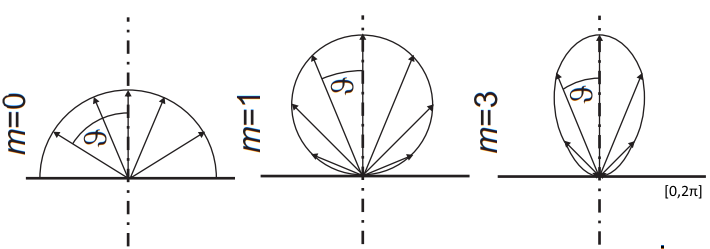
\includegraphics[width=0.8\textwidth]
    {img/strahler.png}
  }
  \caption{Polar profiles for different types of emitters ($m=0$: spherical emitter, $m=1$: Lambert emitter, $m=2$: cone emitter}
  \captionsetup{font={footnotesize,bf,it}}
  \caption*{src: \url{http://www.optik.uni-erlangen.de/odem/vorlesung/ws1213/Photometrie_Geometrische_Optik.pdf}}
  \label{polar}
\end{figure}\vskip 3pt
As a reminder, polar profiles map each angle $\omega$ a magnitude $r$ forming a function $r(\omega)$. They are circular axis versions of the domain $[0..2\pi]$, with negative magnitudes point reflected by 180 degrees. Thus, they are functions with an angular domain making them directionally dependent, which is a well suited representation for point lights (the type of light source with theoretically no finite extend), as we use them in a style of Dachsbacher et al. \cite{dachsbacher}. For the sake of interpretability, we exclude negative values (energies) from the scope of our calculations which we express through mathematical clip functions, limiting negative values to $0.0$, which we denote by subscript $+$ in the following. We will describe the emission charactersitics of point lights exchanging energies in the lattice by parsing such polar functions. Our grid consists of $\mathop{dim}=\mathop{width}\cdot \mathop{height}$ virtual point lights (VPLs), which are in turn light source with (theoretically) no finite extend represented through polar functions. As a start-up thinker for the propagation scheme, we will think of a grid cell in 2D as a center pixel within an 8-neighborhood with a previously injected point light (imagine a spherical emitter: $r(\omega)=1$ here for simplicity). Inside of this cell, we imagine a circular polar profile of radiant intensities for every angle $\omega$ given in $[\frac{W}{\mathop{rad}}]$. Remember, that all considerations from now on are given concerning a single grid cell respectively. Each cell has 8 (4 faces/edges and 4 diagonals) unique neighbors, which are adjacent point lights in the grid (initialized to $I(\omega)=0$). We consider one face neighbor (top) to shortly explain the steps of the scheme. The diagonals and the others are obtained from derivation and symmetry. Naively, one would consider to just transmit the intensity in the direction its pointing into. But this would omit every propagation attenuation principles (any principles at all specifically), if one takes a closer look:
\paragraph{Accumulation stage}
Each cone type (yellow and green) is an individual neighbor-dependent angular area. The diagonals take in a greater angular domain while they are located at greater distance and thus need to be attenuated more strongly (consider an isotropic stimulus). We aim for distributing contributions for overlapping cones to transmit attenuated (because of the larger factor $\sqrt{2}$ distance) intensity in form of a shared part to the diagonals in a single step (which also prevents from zigzagging diagonal intensities in case we would transmit diagonal intensities around the corner). Therefore, the intensity gathered in polar coordinates inside of angular ranges marked in green, needs to be partitioned between 2 of the 8 cone index neighbors with following considerations:

\begin{figure}[!t]
  \centering
 {
    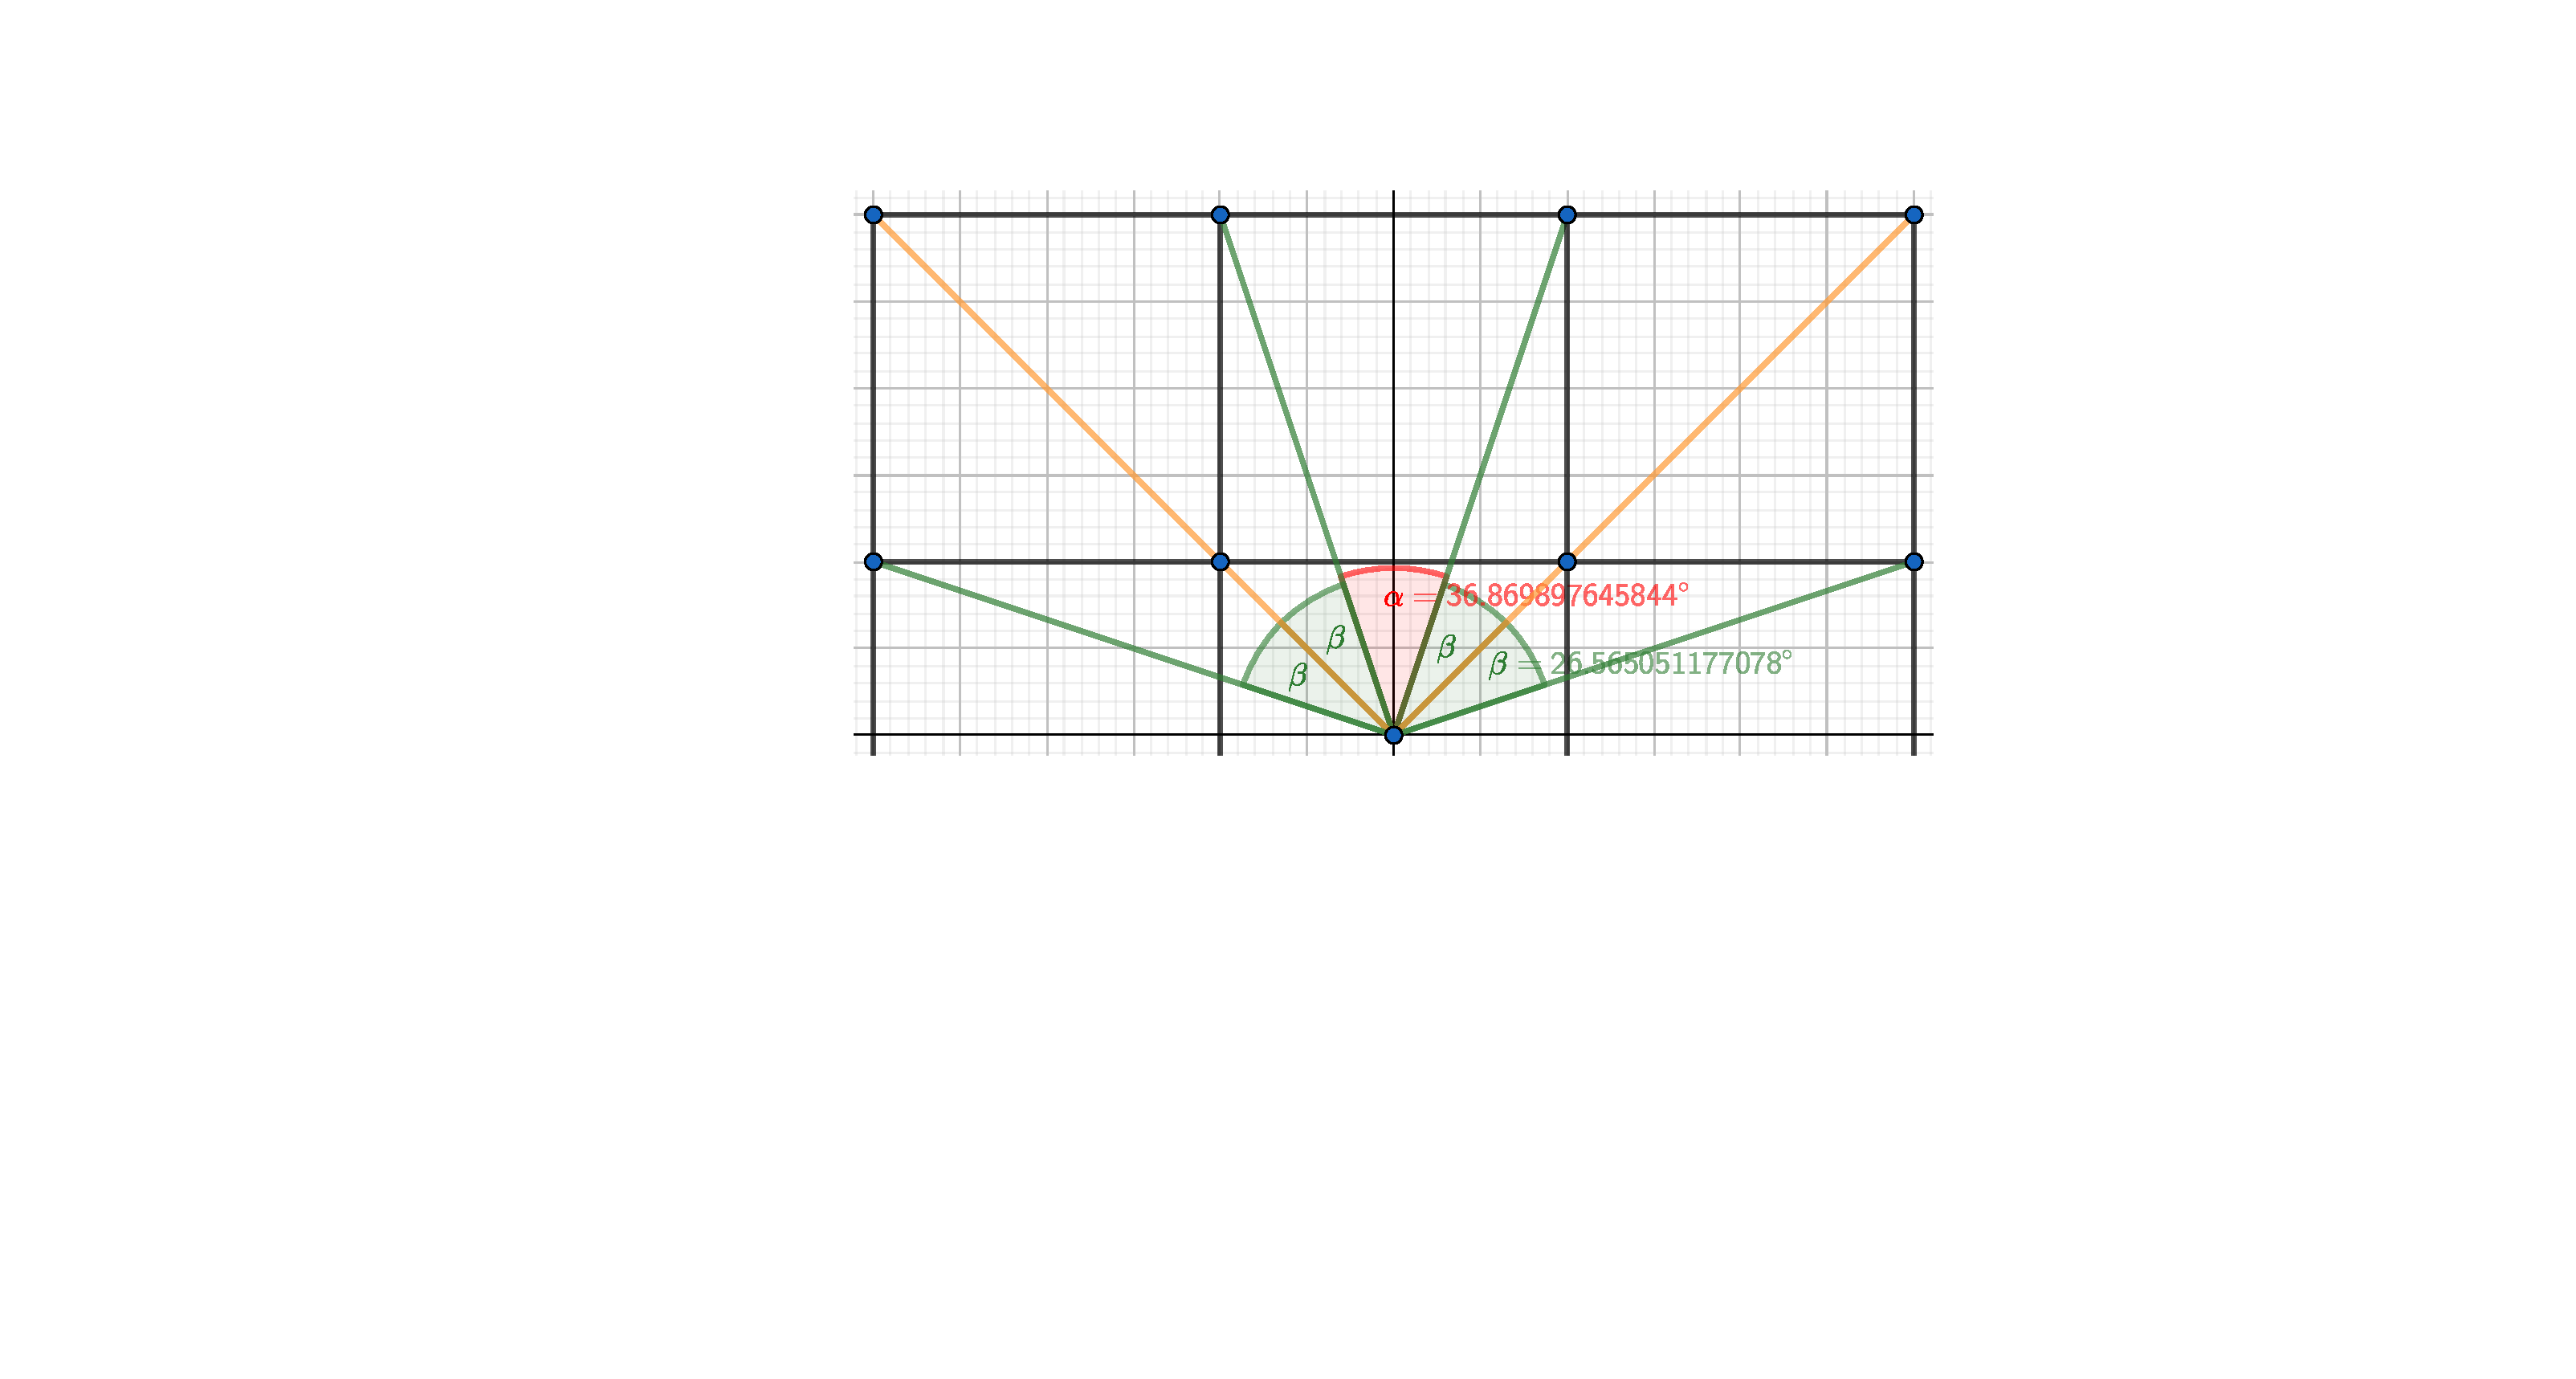
\includegraphics[width=0.8\textwidth]
    {img/geogebra-export_large.pdf}
  }
  \caption{Propagation Scheme}
  \label{scheme}
\end{figure}\vskip 3pt

The face neighbors take in the angular domain of $d_1=\alpha+2\beta$ (yellow cone), whereas the diagonal neighbors (green cones) span a domain of $d_2=2\beta$.
The linear combination weights for the overlapping (green) parts ($\beta$) are obtained from the relative overlapping angular area of the angular span $\beta$ w.r.t. diagonal cones ($2\beta$) and yellow face cones ($\alpha+2\beta = 90^\circ$) (yellow cone is overlapped by green cones at full angle). The linear combination weights are subsequently normalized to $\sum = 1.0$ (normalization condition):
\begin{align}
	\varepsilon_\alpha &= \frac{\frac{\beta}{\alpha+2\beta}}{\frac{\beta}{\alpha+2\beta} + \frac{\beta}{2\beta}} \approx 0.362291\\
	\varepsilon_\beta &= \frac{\frac{\beta}{2\beta}}{\frac{\beta}{\alpha+2\beta} + \frac{\beta}{2\beta}} \approx 0.63771.
\end{align}

Remark, that we can precompute these linear combination weights and reutilize them in each iteration. We define the energetic contributions (presuming the cone is given in local coordinates - i.e. centered around the origin) as follows:
\begin{align}
	\Phi_{\alpha} &= \varepsilon_\alpha\int_\alpha {I}(\omega)\mathop{d\omega} =\varepsilon_\alpha(\int_{-\pi/4}^{-\alpha/2}{I}(\omega)\mathop{d\omega}+\int_{\alpha/2}^{\pi/4}{I}(\omega)\mathop{d\omega})+\int_{-\alpha/2}^{\alpha/2}{I}(\omega)\mathop{d\omega}\\
	\Phi_{\beta} &= \varepsilon_\beta\int_\beta {I}(\omega)\mathop{d\omega} = \varepsilon_\beta\int_{-\beta}^{\beta}{I}(\omega)\mathop{d\omega}
\end{align}

\paragraph{Injection stage}
 We place a cosine lobe scaled with the integrated (accumulated) energies in each of the 8 cone directions (angular domains), whereas outgoing integrated and summed energies are weighted by the linear combination weights (factors) in overlapping (green) areas to split up the contributions accordingly. The contribution areas are depicted in Fig. \ref{scheme}, the cosine lobes can be observed in Fig. \ref{iter} respectively. This manner of propagation is inspired by the propagation scheme of Dachsbacher et al. \cite{dachsbacher} (see the paper on how to ``project the flux into a point light''). Basically, we sum up the weighted intensities corresponding to the respective neighbor index and scale an oriented cosine lobe (in direction of the neighbor) with the total flux $\Phi_t$ accumulated inside the neighbor range to transmit all of the parsed intensity for each neighbor distributed into a cosine distribution. We repeat this process once for each neighbor and each cell respectively. When we are done with the whole grid, we just recursively use the result and keep on running propagation cycles. The implementation is done in a dual buffer approach which pushes the energies back and forth (buffer A to buffer B) for each propagation cyvle until a state of convergence is reached, which is the case when the energy is spreaded throughout the grid and enters a stationary state of equilibrium, characterized by equal out (at grid borders) to in (at light source positions) energy-flow with no more nettings going on inside the domain. We measure the convergence by setting up an overall distribution error w.r.t to the previous iteration. Note that even though we propagate the energy directly through the diagonal cones (which forms a square initially), the 8 degrees of freedom introduce a circular (spherical) wave front after few iterations (for greater resolutions) as depicted in Fig. \ref{iter}. This occurs, because of a faster propagation attenuation which counteracts the larger angle of diagonal cones. There is a redistribution of intensities in the long term resulting in a, since the shared part effects a uniformly spaced isotropic propagation profile resulting in a circular torus-shaped distribution of intensities, as also observed in Fig. \ref{iter}. Also note, that this approach satisfies energy conservation and propagation attenuation principles and applies to the principles of light propagation in vacuum (by default). We infer, that we can assume to follow physical models of spherical waves. The verification of these principal requirements and specifications can be observed in the evaluation in chap. \ref{chap:eval}. We first show the approach for a few iterations with a manual stop criterion to have a kind of imagination for the propagation process:

\begin{figure}[!t]
  \centering
 {
    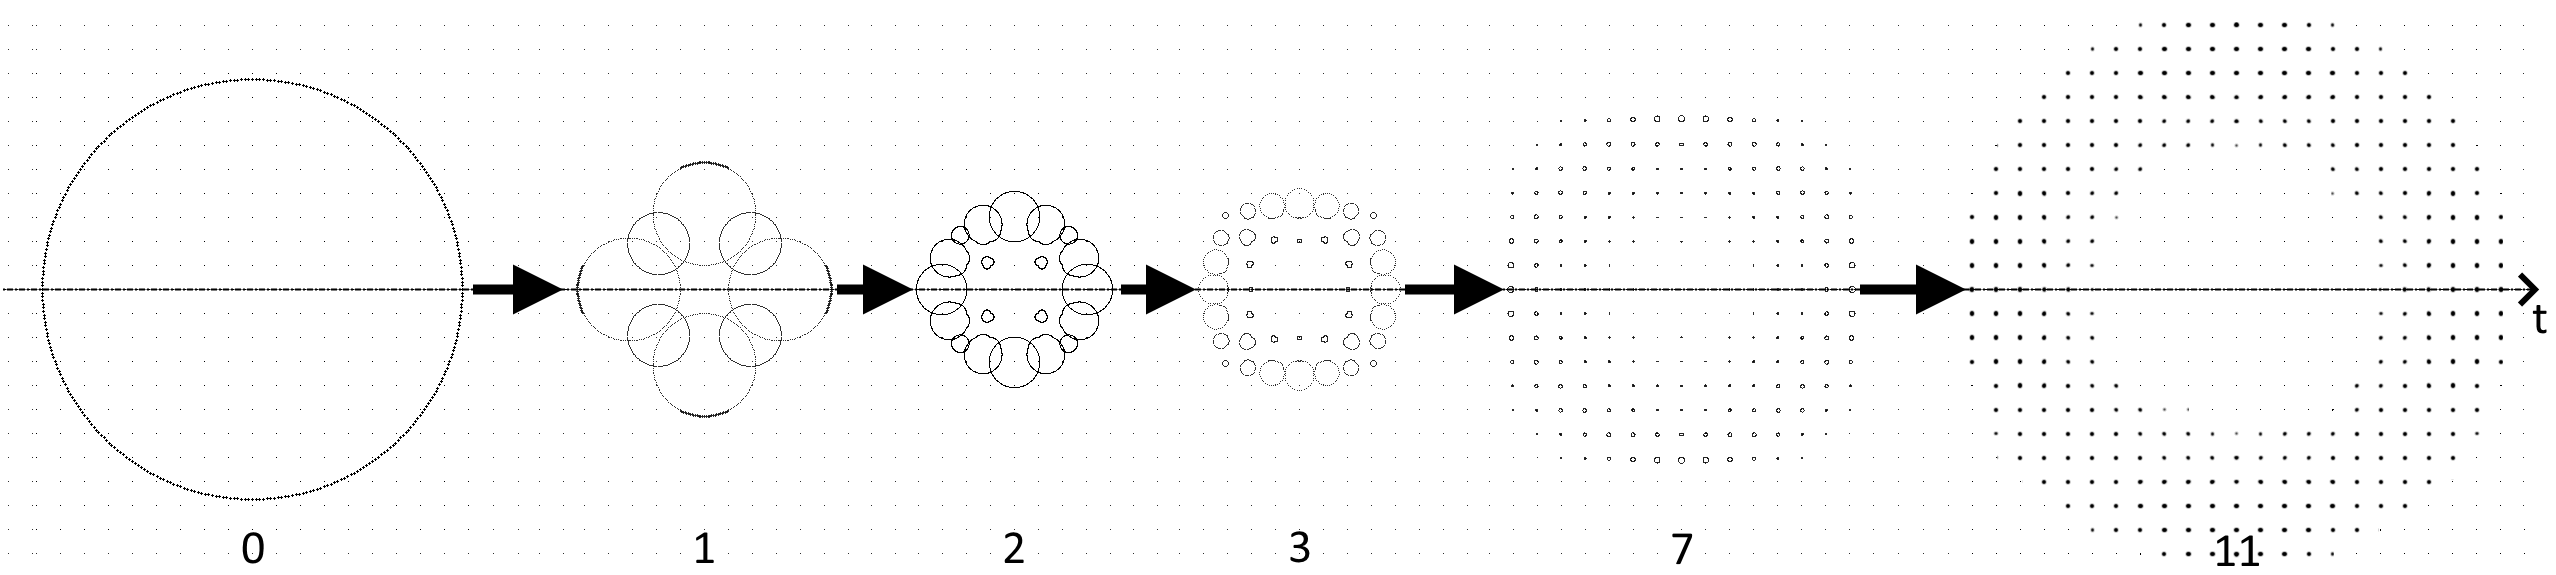
\includegraphics[width=1.0\textwidth]
    {img/steps_gallery_format_arrow_alt.png}
  }
  \caption{Impulse response for isotropic stimulus (few iteration snaphots: $t$)}
  \label{iter}
\end{figure}\vskip 3pt
Fig \ref{iter} depicts the named iteration indices $0,1,2,3,7,11$ (cycles) for the propagation scheme for a circular pulse stimulus which gets turned off after 1 iteration to demonstrate raw energy spreading in the field (impulse response of the algorithm). In step 1 one can observe the placing of cosine lobes scaled with the respective accumulated and weighted energy for the summed area in each of the 8 neighbor directions. In the subsequent steps, remark the evolution from an 8-neighborhood in step 1 to a circular shaped torus.

As already mentioned, a dual-buffer approach is chosen here, as we can efficiently propagate from one into the other and just swap pointers to 
start all over (after reinitialization) until convergence. Another reason is it yields a reasonable source-target or read-write segmentation. We introduce a new operator called \textit{propagate}, permitting us to pre-define the propagation in a symbolic manner. The propagation definition denotes the transformation from one grid (A-buffer) into another (B-buffer) through proper application of the \textit{propagate}-operator to each cell. We will extend this operator with a normalization correction in sect. \ref{sec:trans} in form of a precise mathematical formulation respectively. For now, just imagine the approach in raw operating mode, with no tensor influence incorporated. That is, evaluating and accumulating the polar profiles, weighting with the linear combination weights and scaling and placing of a cosine lobe to the respective neighbor. For now, we want to define our operator $\mathop{propagate}$: Each Grid or Buffer is basically a set of cells defined as $\mathcal{C} = \{\mathbf{c}_1, \mathbf{c}_2, ..., \mathbf{c}_i\}$.  The dual buffer result $\mathcal{C'}$ is denoted symbolically as follows for all cells with a mean intensity greater than zero (those which do not contain trivial null samples):
\begin{align}
	\mathcal{C'} = \mathop{propagate}\{c_i\in \mathcal{C} \ \mid \ |\mean{I}_i| > 0\} \hskip 5pt {\forall } \ i \in [1,\mathop{dim}].
\end{align}
where: $i$: cell index, $I$: source buffer radiant intensity\vskip 5pt
The dual buffer result $\mathcal{C'}$ denotes the set of all transformed cells after the propagation, i.e., after applying the operator $\mathop{propagate}$ to each cell. This result is generated once in each iteration and gets pushed back and forth between the 2 buffers. Note that, $\mathop{dim}=width\cdot height$, which equals the tensor field resolution in this case. At last, we define a threshold for the minimum overall distribution error for the total radiant flux taken into account for a convergence criterion, initiating a stop sequence when falling below that threshold $\epsilon$ (, e.g., $0.5$) :\\
\paragraph{Criterion:}
\begin{align*}
	\Delta \Phi_{total} &= \sum_{c_i\in\mathcal{C}}\lvert\Delta I_i(\omega)\rvert = \sum_{c_i\in\mathcal{C}} \int_0^{2\pi} \lvert(I'_i(\omega)-I_i(\omega))\rvert \mathop{d\omega}  \overset{!}{<} \epsilon\\
\end{align*}
where $\phi_{total}$: total radiant flux, $I'$: target buffer radiant intensity\vskip 5pt
Note that we take the absolute value of the differences to prevent from mutual compensation.

Until now, we aimed to simulate the propagation of light in empty space (vacuum) providing us with a physically-motivated but very simplified base-approach. We aim to modulate the transmission of the intensities on top of the base approach with transmission profiles obtained from the tensor fields through principal component analysis, which yields ellipsoid glyph equations in the following.


%In diesem und den nachfolgenden Abschnitten werden die Beitr�ge der
%Arbeit motiviert, formal sauber (oft mathatisch, sprich mit
%Definitionen etc.) beschrieben, und bei Bedarf mithilfe von Beispielen
%verdeutlicht. Die Beschreibungen in diesem Kapitel sind meist
%unabh�ngig von einer konkreten Realisierung und Daten; diese werden im
%nachfolgenden Kapitel detailliert.

\section{Transmission Profiles and Weighting Functions}
\label{sec:trans}
Note that the following considerations are only given for the tensor profile operating mode with tensor influence incorporated. To obtain a kind of footprint of the tensor field, we set up ellipse equations for each glyph representation, obtained from applying PCA on each cell (tensor) in the grid. Concurrently, we extend our abstract mathematical operator \textit{propagate}, previously referenced in sect \ref{sec:scheme}, by a normalization strategy necessary for windowing weighting profiles, as it is the case for our elliptical transmission profiles, which we will capture in the following. At this point, we presume the precomputation of singular value decomposition and linear combination weights. We map the singular values (corresponding to eigenvalues $\lambda$ here for simplicity) in decreasing order to the ellipses radii (half-axes) $a(\Delta x)$ and $b(\Delta y)$ as follows:

Ellipse Equation:
\begin{align}
	r(\omega) = \frac{ab}{\sqrt{a^{2}\sin^{2}(\omega-\varphi)+b^{2}\cos^{2}(\omega-\varphi)}} =\frac{\lambda_1\lambda_2}{\sqrt{\lambda_1^2\sin^2(\omega-\varphi)+\lambda_2^2\cos^2(\omega-\varphi)}}.
\end{align}
That is, the singular values form the half-axes of the PCA ellipsoid, which yields us a symbolic definition for our transmission (transfer) functions as weighting profiles which we can now evaluate as a parsing and accumulating step. We compute the offset angle $\varphi$ w.r.t. the x-axis by exploiting the $\mathop{atan2}$-function with 4-quadrant evaluation for the first singular vector (ordered decreasingly in value), since we scale the $x$-axis with the first singular value. As a preliminary preparation, this profile is precomputed (sampled) for all discrete angular steps for each cell (, e.g., $360$) and stored for reuitilization as it is the case for the previously mentioned linear combination weights as well. The weighting scheme which we apply is depicted in Fig. \ref{weighting}.
\begin{figure}[!t]
  \centering
  {
    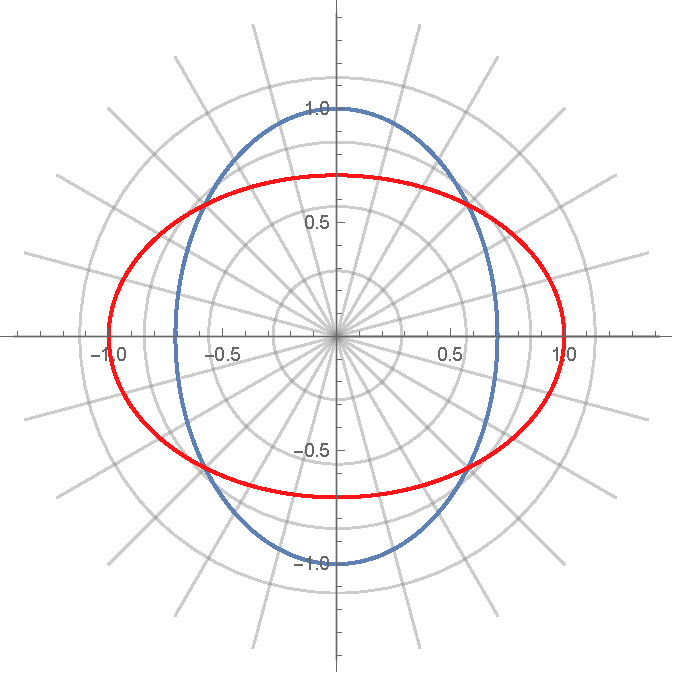
\includegraphics[width=0.5\textwidth]
    {img/polarplot.pdf}
  }
  \caption{red: Intensity Profile, cyan: Transmission Profile (glyph Ellipsoid Eq.)}
  \label{weighting}
\end{figure}
We interpret the polar functions as discrete, sampled 1D vectors with a uniform angular resolution. That means, we can use element-wise multiplication for the 1D-vectors in red (Intensity Profile) and cyan (Transmission Profile) to obtain a windowed version of the intensity profile and perform the following integration step to accumulate the total radiant power (flux) as follows. Note that we model angular dependent radiant intensity ${I}(\omega) [\frac{W}{\mathop{rad}}]$ as an underlying physical entity, which is well suited for describing point light sources. As a side note, the physical quantity perceived as brightness by human eyes, is the radiance (luminance), which is yielded by relating radiant intensity to a finite sensitive area ($[\frac{W}{\mathop{rad}}/m^2]$). The primary definition for our total accumulated incident radiant flux (again presuming that the cone is given in local coordinates - i.e. centered around the origin) is then denoted as:

\begin{align}
	\Phi_{\alpha} &= \varepsilon_\alpha(\int_{-\pi/4}^{-\alpha/2}{T}(\omega){I}(\omega)\mathop{d\omega}+\int_{\alpha/2}^{\pi/4}{T}(\omega){I}(\omega)\mathop{d\omega})+\int_{-\alpha/2}^{\alpha/2}{T}(\omega){I}(\omega)\mathop{d\omega}\\
	\Phi_{\beta} &= \varepsilon_\beta\int_{-\beta}^{\beta}{T}(\omega){I}(\omega)\mathop{d\omega}
\end{align}

This permits us to scale an oriented and clipped cosine-lobe $\cos_+$ with the total radiant flux w. respect to its own total energy when integrated likewise. A discrete cosine lobe never reaches its theoretical sum of $2$ exactly in the interval $[{-\frac{\pi}{2}},{\frac{\pi}{2}}]$. Therefore it needs to be computed to account for sampling (discretization) errors and normalized by following relation (, e.g., $\sum_{\cos} \approx 1.9949204635834517$).
\begin{align}
\sum_{\cos_+} &= \int_{-\frac{\pi}{2}}^{\frac{\pi}{2}}\cos_+(\omega)\mathop{d\omega} \approx 2,\\
	\cos_k(\omega) &= \frac{\Phi_t}{\sum_{\cos_+}}cos_+(\omega-k\cdot\frac{\pi}{4})\hskip 20pt w. \ k\in[0,7].
\end{align}
This specific profile is injected in form of a placement to the corresponding neighbor index $k$. It yields a cosine lobe, which has an overall energy of $\Phi_t$, if the point light is interpreted with a Lambert-emitter (cf. \cite{lindlein}) characteristic (as part or area element of a diffusely reflecting surface) since the intensity profile matches a cosine in this case. This emitter characteristic is the case for global illumination diffuse indirect illumination (non-specular). It is used in similar style by Dachsbacher et al. for propagating intensities through LPVs (light propagation volumes).
But caution, we should not generate any exceeding energy right? Now each tensor ellipse equation has a mean transmission rate $[\%]$, which turns out to be a measure or synonym for the total rate of the outgoing transmitted radiant intensity $\int_0^{2\pi}{T}(\omega)\mathop{d\omega}$. Since energy can not be generated from transmission profiles (only transmitting, not generating), we have to normalize every tensor ellipse equation with the highest mean transmission rate in the field, which is then transmitting the whole outgoing intensity $\int_0^{2\pi}{I}(\omega)\mathop{d\omega}$ in total. This restricts the tensor ellipse mean to a maximum of $100\%$ for the tensor with the highest tensor magnitude. We will use the self-made definition of mean tensor magnitude $\mean{r}_{max}$ obtained from the PCA here for simplicity. That is, we take the principal component ellipsoid and calculate its analytical mean, which is then used for mean normalization to $\mean{r}_{max}=1.0$. Hence the tensor ellipse equations are normalized through the following step:
\begin{align}
	r_n(\omega) = \frac{1}{\mean{r}_{max}}r(\omega).
\end{align}
Notice, that this implements the concept of absorption implicitly, because tensors with a lower mean $\mean{r}$ than $100\%$ absorb energy wheras absorption equals ${\mu} = {1}-{\mean{r}}$ here. Now that we have coped with the problem of overall transmission, we are left with another problem that occurs with the weighting functions as they can still yield values above $1.0$. Consider following examples as $T(\omega)I(\omega)$ pairs (obviously normalized to $1.0$): $1.5\cdot 1.5=2.25$ and $0.5\cdot 0.5=0.25$, which disproves us that a mean $\bar{r}=1.0$ necessarily effects a mean transmission intensity $I_t$ of $1.0<1.25=\frac{2.5}{2}$. This would potentially generate intensity out of nothing which leads to crucially unstable behaviour, since we employ uncontrolled sources of energy in this case. Well, but only in case energy conservation principles were not respected.  To construct a solution, we ask for the source of the excessive energy. If the tensor mean complies with the constraint $\mean{r}\leq 1.0$, then the energy must lack in some other place (since the overall transmission fulfills the energy conservation constraint in that case). The only problem is that a normalization condition in usual style for the transmission profile ${T}(\omega)$ does not necessarily imply the same normalization for the term ${T}(\omega){I}(\omega)$. However, a proper normalization can provide corrective support, wich reveals another subsequent normalization constraint. The normalization factor is defined in 3 subsequent steps:
\begin{enumerate}
	\item Normalization of $TI$ to $\overline{TI}=1.0$
	\item Subsequent scaling w. mean intensity $\mean{I}$ for energy conservation principles
	\item Subsequent scaling w. mean tensor magnitude $\mean{T}$ for absorption principles
\end{enumerate}

Hence the transmitted outgoing intensity for a single direction is defined as:

\begin{align}
    {I}_t(\omega) = 
\begin{cases}
   n_f\varepsilon_\alpha{T}(\omega){I}(\omega),& \text{if } k\bmod 2 = 0\\
     n_f\varepsilon_\beta{T}(\omega){I}(\omega),              & \text{otherwise}
\end{cases}
\end{align}

This transforms our equation for the transmitted radiant flux into:
\begin{align}
	\Phi_{\alpha,t,i} &= \int_\alpha{I}_{t,i}(\omega)\mathop{d\omega} = n_f\Phi_{\alpha,i},\\
	\Phi_{\beta,t,i} &= \int_\beta{I}_{t,i}(\omega)\mathop{d\omega} = n_f\Phi_{\beta,i}.
\end{align}
Which is now respecting energy conservation principles very conveniently, as all we need is a set of means and we are capable of normalizing the weighted intensity profile transmitted. This collapses our abstract mathematical operator $\mathop{propagate}$, which is applied to each cell, into the following steps:
\begin{enumerate}
	\item Computation of normalization factor $n_f$
	\item Direction (component)-wise weighting to account for shared part in diagonal cones
	\item Integration (accumulation) of total radiant flux weighted with \underline{normalized} transmission profiles inside the angular neighbor range (read-access)
	\item Scaling of cosine lobe corresponding to neighbor direction and subsequent placing (injection) to corresponding neighbor (write-access)
	
\end{enumerate}
Remember that this operator needs to applied once to each cell to form a whole propagation cycle propagating intensities from source to target buffer. This approach ensures that no energy will be generated and therefore implements the 	physical law of energy conservation or Kirchhoff's current law if you want to think of a particle's diffusion process. Consequently, this allows us to assume that all sources of power (energy) are user-defined. In fact the approach has proven to be robust w.r.t. energy losses for several iterations as depicted in chap. \ref{chap:eval} in the stochastic error graph.

\section{Physical Model}
\label{sec:model}
To constitute a physical interpretation for the transmission of the tensor field, we imagine a melting crystal with  fibrous structures aligning with the major eigenvectors of the tensor field. This is what we call the footprint of the tensor field. In that sense of imagination, we would virtually imprint every tensor field into a crystalline structure as a preliminary initialization step. For an every day example, this can be observed in, e.g., the gemstone tiger's eyes' cat's eye effect, where crystal fibers align with the crystal axes respectively and effect a brightened line which never changes position or orientation when rotating the crystal. These oriented crysal fibers are then representing the biased propagation directions of light inside of the crystal lattice. The propability density function $P(\omega)$, for a photon being scattered in a particular direction $\omega$ \ref{ryder}, is then described as:
\begin{align}
 	P(\omega) &= \frac{T(\omega)}{\int_{k\pi}^{(k+1)\pi}T(\omega)\mathop{d\omega}}\\
 	w. \int_0^{\pi} P(\omega) &= 1.
\end{align}
This propability density function (PDF) indicates, whether there is directed anisotropy or spherical isotropy w.r.t the neighboring $180$ ($\pi \mathop{rad}$) degrees and how likely the spontaneuos scattering of a photon in this particular direction will happen. Each tensor is then a unique footprint which can be precomputed for convenience and described as polar profile just as our previously mentioned intensity profiles. We apply these polar profiles in a sense of transmission profiles as discussed in sect. \ref{sec:trans}.

\section{Light Propagation Scheme Behaviour}
To evaluate the plausibility of the light distribution results obtained from the light propagation scheme, we plot the transmission profiles overlaid with the resulting intensity profiles for several synthetic test fields, whereas red: tensor glyphs (transmission profiles) and blue: intensity profiles are both depicted in polar coordinates:
\begin{figure}[!t]
\centering
  \begin{minipage}{0.4\textwidth}
    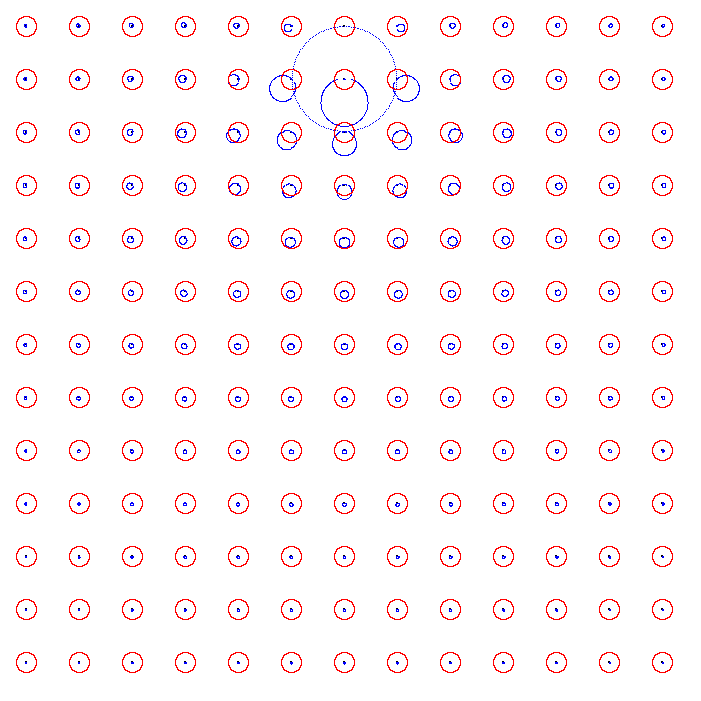
\includegraphics[width=0.8\textwidth]{img/isotropic.png}
    \label{a)}
    \caption*{light src in top center}
  \end{minipage}
  \begin{minipage}{0.4\textwidth}
    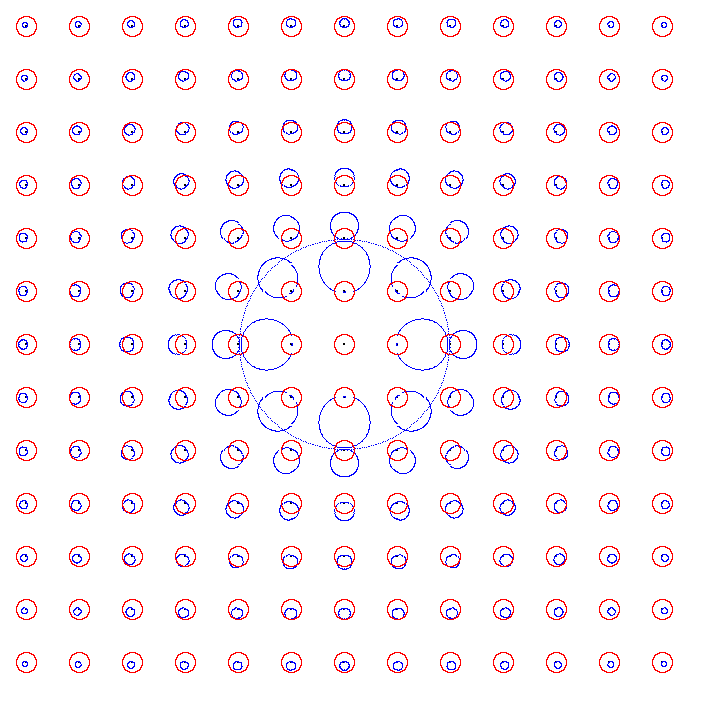
\includegraphics[width=0.8\textwidth]{img/isotropic-all-center.png}
    \label{b)}
    \caption*{light src in center}
  \end{minipage}
\caption{final light propagation distributions for ``isotropy''-testfield}
\label{isotropic}
\end{figure}
One can observe here, how light is propagated with no directional bias leading to an absolutely isotropic distribution in case  b), which is symmetric as expected. This result is considered to be the absolute ground truth example for the light propagation scheme, which is evaluated separately in sect. \ref{sec:att} and \ref{sect:conserve}. We can also depict the final distribution as a scalar field when using the total energy in each cell as scalar:

\begin{figure}[!t]
\centering
  \begin{minipage}{0.4\textwidth}
    \centering
    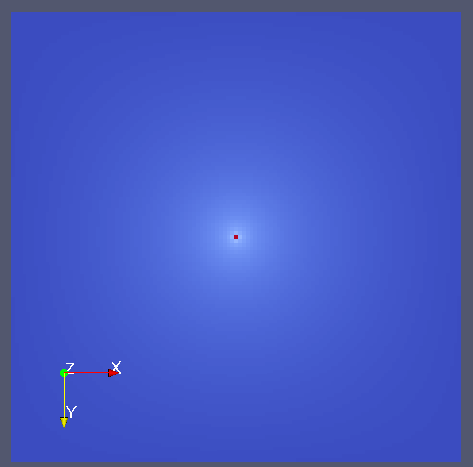
\includegraphics[width=0.9\textwidth]{img/iso_scalar.png}
    \label{a)}
    \caption*{light src in center}
  \end{minipage}
  \begin{minipage}{0.4\textwidth}
    \centering
    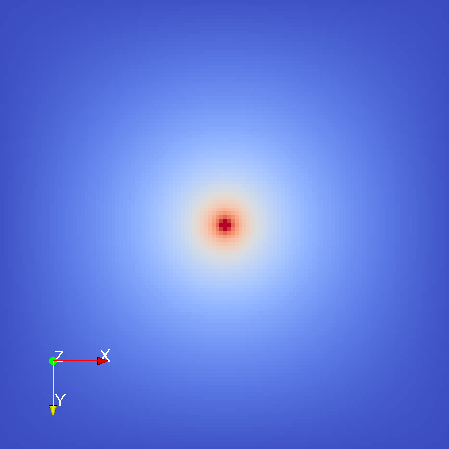
\includegraphics[width=0.9\textwidth]{img/iso_sat.png}
    \label{b)}
    \caption*{light src in center (rescaled)}
  \end{minipage}
\caption{final light distributions for ``isotropy''-test field}
\label{rings-tests}
\end{figure}
Note that we skipped the top center example, since we consider it a trivial add-on example. When we observe these scalar heat map plots, we first notice the red dots, which always represent light sources (since they are captured the most energy) in these cases. Specifically, the heat maps are obtained from the same light distributions we plot as polar profiles and should hence be interpreted concurrently. Remark the propagation front indicating a circular wave (circular isolines in a)).
In this next example, we use the tensor field ``rings'' as input data for the approach and observe how the intensities are channeled in a circular orbit around the central origin. The anisotropy measures decide whether the transmission profile is more narrow (radical) or more wide (liberal):
\begin{figure}[!t]
\centering
  \begin{minipage}{0.4\textwidth}
    \centering
    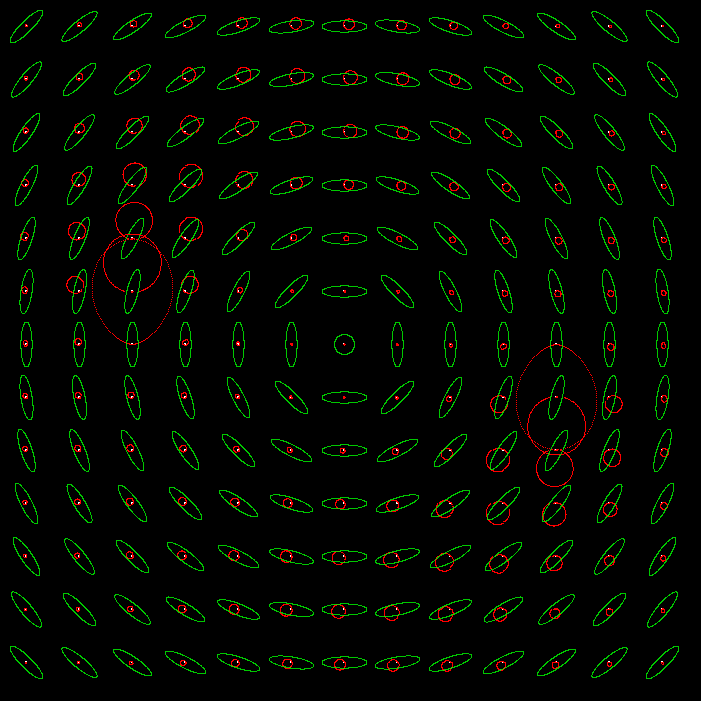
\includegraphics[width=0.9\textwidth]{img/rings-two-special1.png}
    \label{a)}
    \caption*{antisymmtric light src's}
  \end{minipage}
  \begin{minipage}{0.4\textwidth}
    \centering
    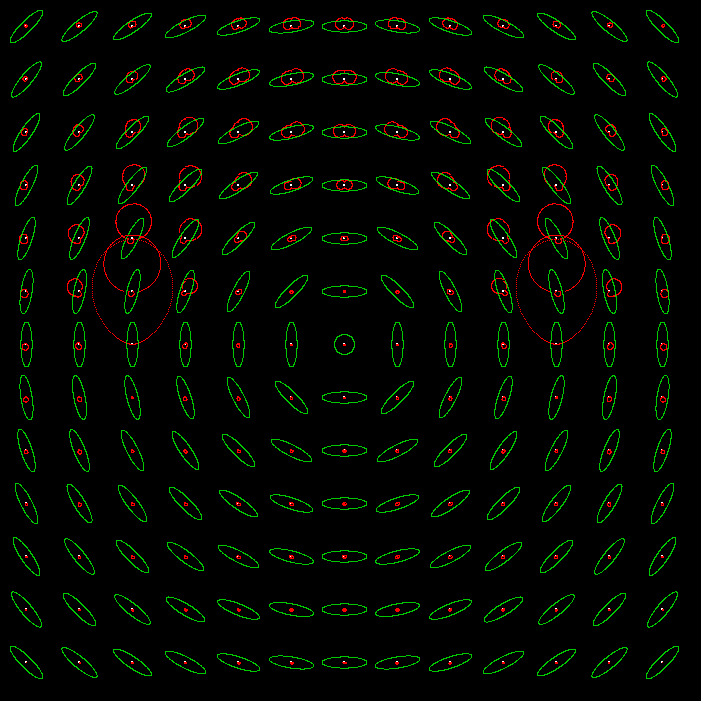
\includegraphics[width=0.9\textwidth]{img/rings-two-special2.png}
    \label{b)}
    \caption*{symmetric light src's}
  \end{minipage}
\caption{final light propagation distributions for ``rings''-test field}
\label{rings-tests}
\end{figure}
We consider Fig. \ref{rings-tests} to regard the behavior for circular tensor field lines. As expected, the intensities get directed in circular orbits by the tensor ellipsoid transmission profiles. Note the symmetry for both cases depicted. Again, we plot the final light distributions as heat maps:
\begin{figure}[!t]
\centering
  \begin{minipage}{0.4\textwidth}
    \centering
    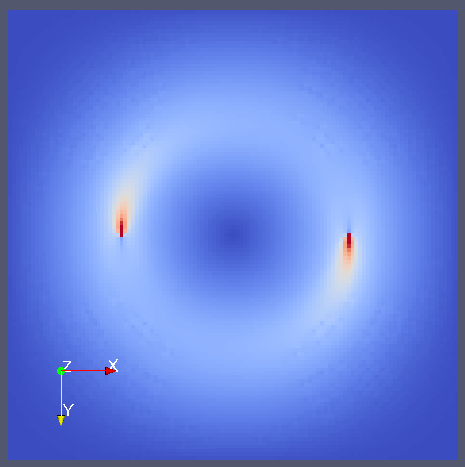
\includegraphics[width=0.9\textwidth]{img/cos_parallel.png}
    \label{a)}
    \caption*{antisymmtric light src's}
  \end{minipage}
  \begin{minipage}{0.4\textwidth}
    \centering
    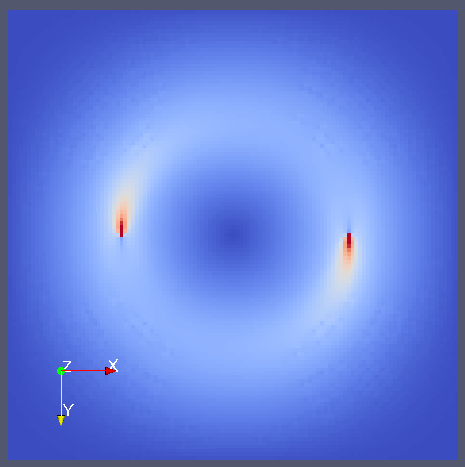
\includegraphics[width=0.9\textwidth]{img/cos_anti.png}
    \label{b)}
    \caption*{symmetric light src's}
  \end{minipage}
\caption{final light propagation distributions for ``spiral''-test field}
\label{spiral-tests}
\end{figure}
It is noticeable, that the intensities concentrate preferably on the circular tensor field lines, which proves the approach's controlling ability expressing as direction.
The results for our tensor field ``spiral'' can be interpreted in analogous fashion as the previously discussed ``rings''-testfield. The influence incorporated by the tensor field is easily noticeable in this case as well:
\begin{figure}[!t]
\centering
  \begin{minipage}{0.4\textwidth}
    \centering
    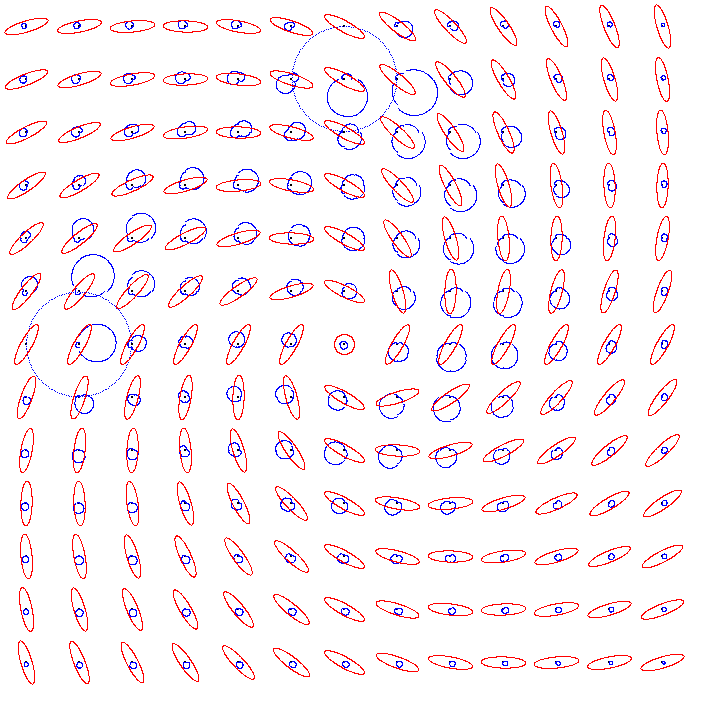
\includegraphics[width=0.9\textwidth]{img/spiral-two-dense.png}
    \label{a)}
    \caption*{dense light src's}
  \end{minipage}
  \begin{minipage}{0.4\textwidth}
    \centering
    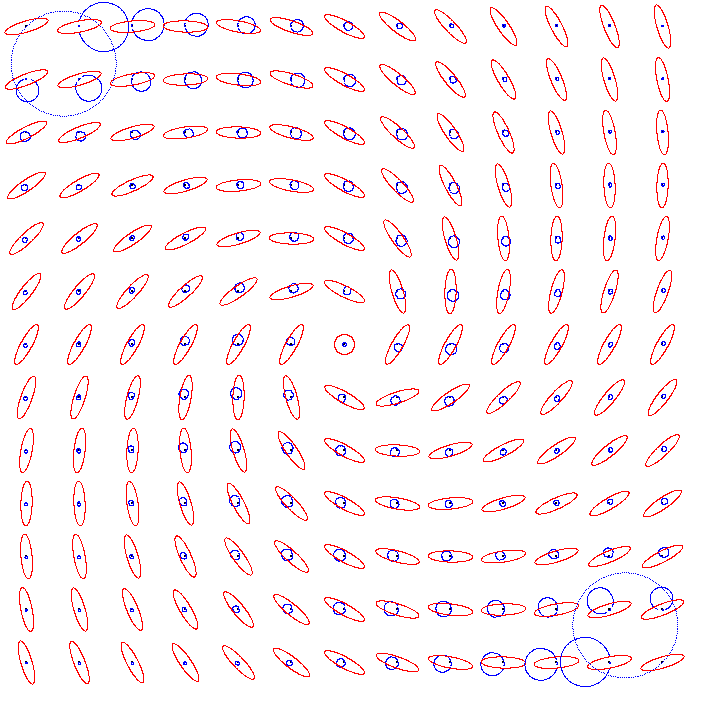
\includegraphics[width=0.9\textwidth]{img/spiral-two-wide.png}
    \label{b)}
    \caption*{symmetric light src's}
  \end{minipage}
\caption{final light propagation distributions for ``spiral''-test field}
\label{spiral-tests}
\end{figure}
For the ``spiral'' tensor field we observe the spiral shape literally absorbing the intensities into its spiral arms, which becomes even more clear when we again observe the heat map representation:
\begin{figure}[!t]
\centering
  \begin{minipage}{0.4\textwidth}
    \centering
    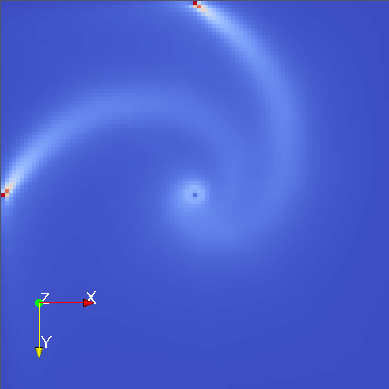
\includegraphics[width=0.9\textwidth]{img/spiral-temp2.png}
    \label{a)}
    \caption*{dense light src's}
  \end{minipage}
  \begin{minipage}{0.4\textwidth}
    \centering
    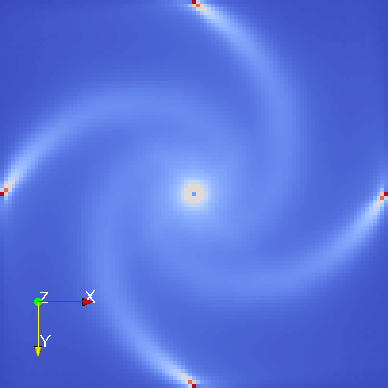
\includegraphics[width=0.9\textwidth]{img/spiral_full.png}
    \label{b)}
    \caption*{four light src's}
  \end{minipage}
\caption{final light propagation distributions for ``spiral''-test field}
\label{spiral-tests}
\end{figure}

The star example reveals another interesting feature of the approach: if the intensity impulsively hits an isotropic region, it gets directed according to its intensity profile (neglecting the transmission profile) which implements the principle of inertia for directed light propagation present in vacuum (light never changes its direction):
\begin{figure}[!t]
\centering
  \begin{minipage}{0.31\textwidth}
    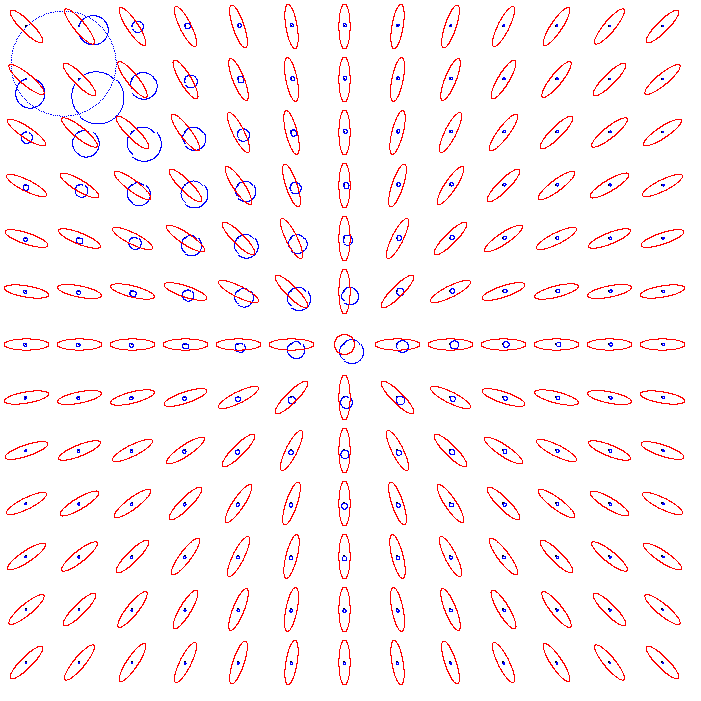
\includegraphics[width=\textwidth]{img/star-0,0.png}
    \label{a)}
    \caption*{single light src}
  \end{minipage}
  \begin{minipage}{0.31\textwidth}
    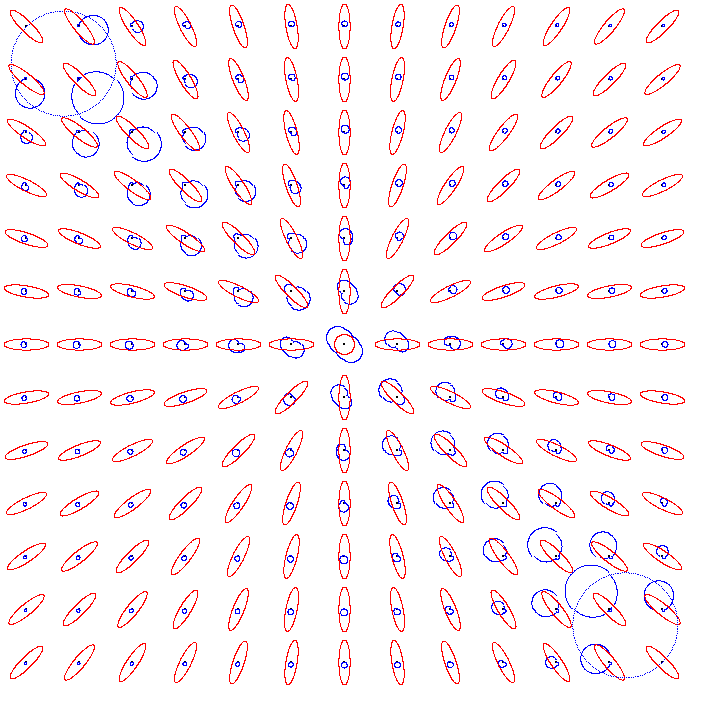
\includegraphics[width=\textwidth]{img/star-two-wide.png}
    \label{b)}
    \caption*{symmetric light src's}
  \end{minipage}
   \begin{minipage}{0.31\textwidth}
    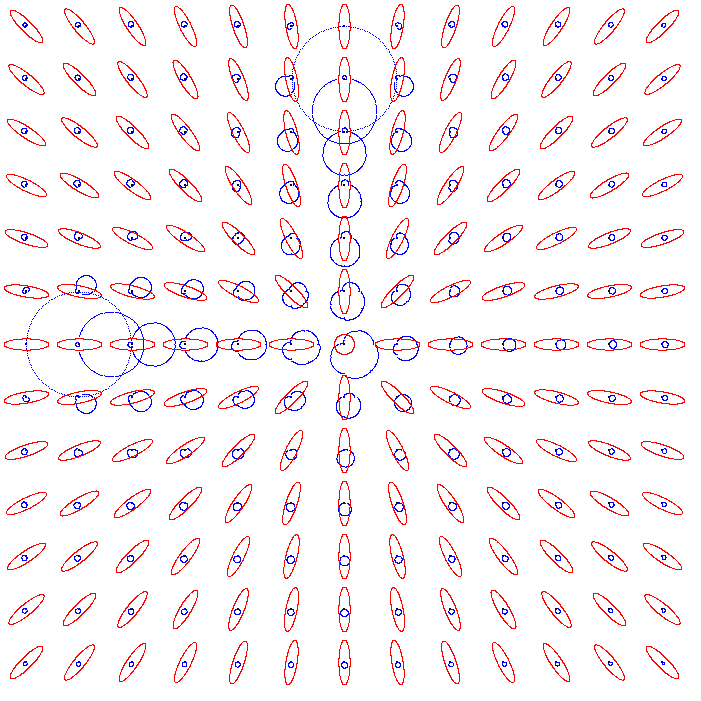
\includegraphics[width=\textwidth]{img/star-two-dense.png}
    \label{c)}
    \caption*{dual light src's}
  \end{minipage}
\caption{final light propagation distributions for ``star'' test field}
\label{spiral-tests}
\end{figure}
Remark, that the diagonal intensities are attenuated more strongly by default, which introduces a bias into the light paths which are chosen along the axes with higher propability, effectively. This gets even clearer, when we plot the heat map depiction again:
\begin{figure}[!t]
\centering
  \begin{minipage}{0.31\textwidth}
    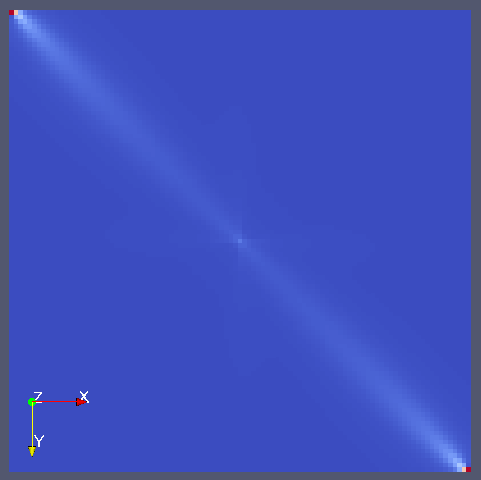
\includegraphics[width=\textwidth]{img/star_wide.png}
    \label{a)}
    \caption*{symmetric light src's}
  \end{minipage}
  \begin{minipage}{0.31\textwidth}
    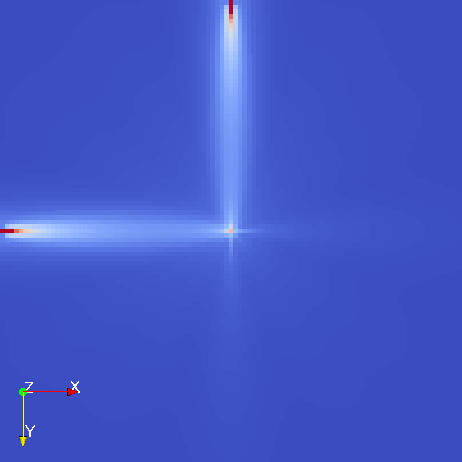
\includegraphics[width=\textwidth]{img/star_close.png}
    \label{b)}
    \caption*{dual light src's}
  \end{minipage}
\caption{final light propagation distributions for ``star'' test field}
\label{spiral-tests}
\end{figure}
Note that we skipped the single light source example, since we consider it a trivial add-on example. We can regard the intensities condensed inside of a narrow beam of light.
Note, that a logarithmic scale needs to be incorporated to produce results on a large scale in a sense of higher spatial resolution (e.g. $101\times 101$), since the propagation attenuation follows the distance to the origin inversely proportional.

\section{Light Transport Gradient (LTG)}
\label{sec:ltg}
\subsection{Evolution}
Now, that we are able to propagate intensity in grid, directed by the eigenvectors of the tensor field, we aim to do something more elaborate to segment ROIs (regions of interest) characterised by divergence/convergence of tensor field lines and drastic changes in anisotropy. For this purpose, we imagine kind of a local and spatial gradient, as we place light sources in two close-by positions and eventually in two close-by directions and analyze the resulting final light distribution. We consider the light distributions and their difference image for the \enquote{isotropic} and the \enquote{drain} test field to have an idea, for which kind or types of cases/configurations we obtain inherently different light distributions, in particular.  We choose to use these test cases, because they constitute absolutely pure examples par excellence for a FTLE computation exposing no (\enquote{isotropic}), or on the other hand raw (\enquote{drain}) tensor field lines diverging. We will start off with the \enquote{isotropic} field from here to first analyze the offset response for no divergence or more specifically, no anisotropy at all. Fig. \ref{analysis1} depicts final light distributions (cf. sect. \ref{sec:ltg} Fig. \ref{rings-tests}) for placing the light source one step to the left and one to the right from the central axis (spatial offset). We can observe the light cones cancel out each other in the center of the difference image. That is, per default, light distributions cancel each other out for two close-by light source positions or directions (or more specifically: for continous overlaps in their distributions). In this case, for the \enquote{isotropic} test field, we have no tensor field lines diverging leading to a small overall difference for light sources in finite distance. 

\begin{figure}[!t]
\centering
  \begin{minipage}{0.3\textwidth}
    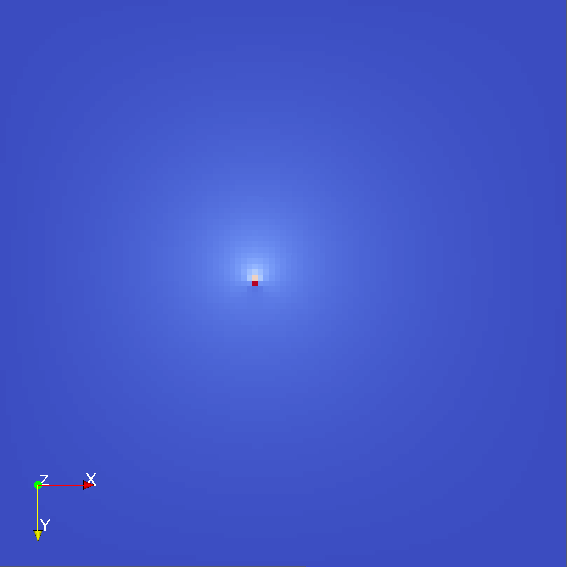
\includegraphics[width=\textwidth]{img/scalar_iso_left.png}
    \label{a)}
    \caption*{a) final light distribution for left spatial offset}
  \end{minipage} $-$
  \begin{minipage}{0.3\textwidth}
    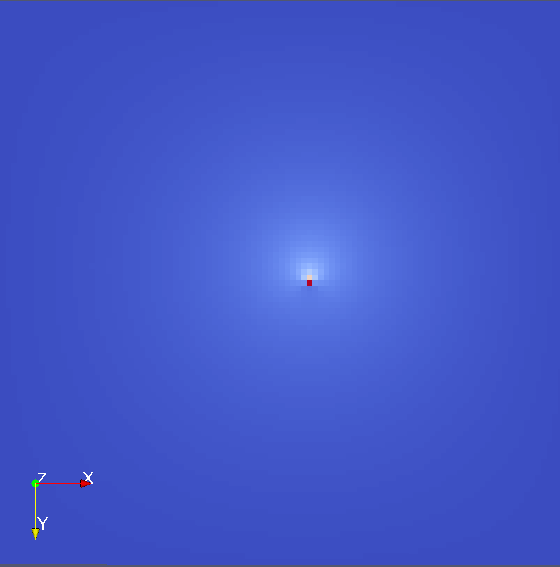
\includegraphics[width=\textwidth]{img/scalar_iso_right.png}
    \label{b)}
    \caption*{b) final light distribution for right spatial offset}
  \end{minipage} $=$
   \begin{minipage}{0.3\textwidth}
    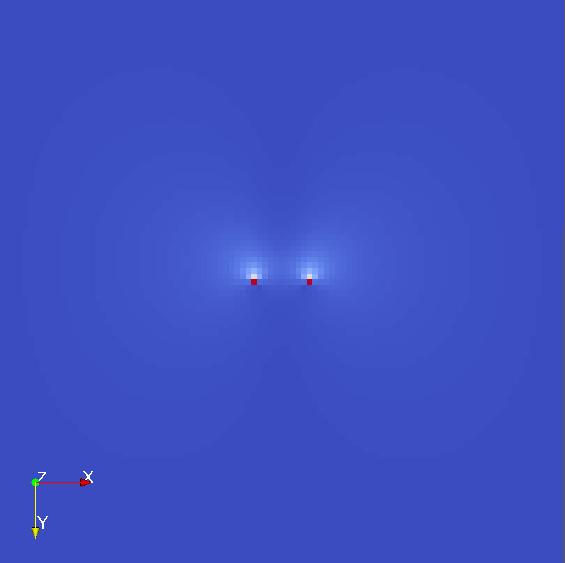
\includegraphics[width=\textwidth]{img/scalar_iso_diff.png}
    \label{b)}
    \caption*{difference image for a) and b)}
  \end{minipage}
  \caption{``isotropic'' test field}
\label{analysis1}
\end{figure}

The complementing idea for the angular domain would be: placing the light source at the same position but pointing in differing directions, which is depicted in Fig \ref{analysis2}.
\begin{figure}[!t]
\centering
  \begin{minipage}{0.3\textwidth}
    \includegraphics[width=\textwidth]{img/scalar_iso_leftangle.png}
    \label{a)}
    \caption*{a) final light distribution for left angular offset}
  \end{minipage} $-$
  \begin{minipage}{0.3\textwidth}
    \includegraphics[width=\textwidth]{img/scalar_iso_rightangle.png}
    \label{b)}
    \caption*{b) final light distribution for right angular offset}
  \end{minipage} $=$
   \begin{minipage}{0.3\textwidth}
    \includegraphics[width=\textwidth]{img/scalar_iso_anglediff.png}
    \label{b)}
    \caption*{difference image for a) and b)}
  \end{minipage}
  \caption{``isotropic'' test field}
\label{analysis2}
\end{figure}
For the angular offset, we can again observe the light distributions cancelling each other out (per default) in the center (middle) of the difference image. For now, we can take home from these examples, that light distributions are cancelling each other out within their overlap in general, in case no anisotropy was introduced into the test tensor field. We again analyze the drain test field (cf. Fig. \ref{drain} in sect. \ref{chap:grundlagen}) for the behavior of the resulting light distributions in scalar field representation. This following example illustrated in Fig. \ref{evolution1} now introduces raw tensor field lines diverging w.r.t. the $y$-axis.

\begin{figure}[!t]
\centering
  \begin{minipage}{0.3\textwidth}
    \includegraphics[width=\textwidth]{img/ftle_left.png}
    \label{a)}
    \caption*{a) final light distribution for left spatial offset}
  \end{minipage} $-$
  \begin{minipage}{0.3\textwidth}
    \includegraphics[width=\textwidth]{img/ftle_right.png}
    \label{b)}
    \caption*{b) final light distribution for right spatial offset}
  \end{minipage} $=$
   \begin{minipage}{0.3\textwidth}
    \includegraphics[width=\textwidth]{img/ftle_diff.png}
    \label{b)}
    \caption*{difference image for a) and b)}
  \end{minipage}
  \caption{``drain'' test field}
\label{evolution1}
\end{figure}
We can see the light distributions diverge following tensor field lines, which �n turn form these curves depicted in Fig. \ref{evolution1}. The separation of path (tensor field) lines and thus of light distributions is maximized at the center location of the field. We can now examine the light paths being dragged into long curves, which prevents the light distributions from overlapping at all. Hence, this test case will lead to larger differences and thus to an increased response of the FTLE field, which we will define in this section. 
%Imagine accumulating each pixel in the images to obtain the cumulative total energy in the (difference) grid, which could now be compared for each light source position and direction in terms of proper min-max scaling.

\begin{figure}[!t]
\centering
  \begin{minipage}{0.3\textwidth}
    \includegraphics[width=\textwidth]{img/ftle_leftangle.png}
    \label{a)}
    \caption*{a) final light distribution for left angular offset}
  \end{minipage} $-$
  \begin{minipage}{0.3\textwidth}
    \includegraphics[width=\textwidth]{img/ftle_rightangle.png}
    \label{b)}
    \caption*{b) final light distribution for right angular offset}
  \end{minipage} $=$
   \begin{minipage}{0.3\textwidth}
    \includegraphics[width=\textwidth]{img/ftle_anglediff.png}
    \label{b)}
    \caption*{difference image for a) and b)}
  \end{minipage}
  \caption{``drain'' test field}
\label{evolution2}
\end{figure}
For the angle, we can observe again that the difference is again increased, but does not 
Imagine accumulating each pixel in the images to obtain the cumulative total energy in the (difference) grid, which could now be compared for each light source position and direction in terms of proper min-max scaling. Now imagine we would accumulate these differences and assign each position a gradient magnitude in form of a scalar value with the summed difference of the final light distributions in the neighborhood. What would we eventually be yielded with. Well, we would obtain another scalar field considered to be the gradient image of the light distributions. We could very well extend this process for every light source direction discretized (sampled) and obtain a $3D$ volume representing the topological structure of the tensor field for every direction. All we need, is a formal definition for a central differences gradient approximation for light distributions given in polar profiles. The main difference to FTLE in vector field visualization is, that we use whole distributions of trajectories and hence need to use a starting direction for the distribution of trajectories, instead of just moving with the flow, as a tensor introduces a whole distribution of directions and does not only depend on the inital position, but also on the direction. This corresponding to the volume emerging from the FTLE plane image, as we introduce a new dimension $\omega$.

Remark that we denote the final buffer result as $\mathbf{b}=\mathcal{C}_{final}$ in the following.
\subsection{Definition}
 As tensor field lines are bidirectional, convergence and divergence can not be reasonably discerned in that case. We aim to extract ridges from a FTLE-like field to grasp the key regions separating anisotropy behavior (, i.e., changes in direction/tensor magnitude) in the field segmented as height ridges in the field, which are in turn LCS (Lagrangian Coherent Structures) well known for their rich substance in physical meaning. They often indicate transport barriers in flow fields. The nature and location of these structures and their interaction with each other is subject to the study of both turbulent and laminar mixing. They can even be observed in nature for, e.g., vortices in flow fields. For this purpose, we will use our, previously defined, $\mathop{propagate}$-operator, i.e., the propagation scheme from sect. \ref{sec:scheme} and \ref{sec:trans}, on every possible light source location $\mathbf{x}$ and direction $\omega$ in the grid to obtain the final set of buffers $\mathcal{B} = \{\mathcal{C}_1, \mathcal{C}_2, ..., \mathcal{C}_j\}$ of impulse responses of the algorithm. That is, we initialize the grid with every possible light source configuration and compute a whole final light distribution for each step:
\begin{align}
	\mathcal{B} = \mathop{propagate}\{c_i\in \mathcal{C} \ \mid \ |\mean{I}_i| > 0\} \ {\forall } \ i \in [1,\mathop{dim}] \ {\forall } \ j \in [1,\mathop{dim}\cdot \mathop{steps}].
	\label{ftle}
\end{align}
Whereas $j$ is the index of light source position and direction representing the initialization in each iteration and $\mathop{steps}$ is the count of the discrete angular steps. The initialization is done by placing a light src (delta-impulse) with $\mean{I}_i = 1.0$ at the exact location of index $j$ realizing a light source at location $(x\mid y)$ in direction $\omega$. Eq. \ref{ftle} now denotes the set of buffers $\mathcal{B}$ containing light distributions propagated from, i.e., computed for every possible direction and location. Now, that we have measured impulse responses from every location in our long $1D$ sample vector, we can incorporate finite (central) differences to obtain the gradient of the set of final buffers with final light distributions as elements $\mathcal{C}_{final}=\mathbf{b}\in\mathcal{B}$. Note, that we interpret a finite set $\mathcal{C}_{final}$ as a vector of cells $\mathbf{b}$ with concurrent indices here:
\begin{align}
	\nabla \mathbf{b}_{x,y,\omega} =
	\begin{pmatrix}
	\frac{\partial \mathbf{b}_{x,y,\omega}}{\partial x} \\ \frac{\partial \mathbf{b}_{x,y,\omega}}{\partial y} \\ \frac{\partial \mathbf{b}_{x,y,\omega}}{\partial \omega}
	\end{pmatrix} \approx
	\frac{1}{2}
	\begin{pmatrix}
	\sum_{\mathbf{c}}\lvert \mathbf{b}_{x+1,y,\omega} - \mathbf{b}_{x-1,y,\omega}\rvert \\ \sum_{\mathbf{c}}\lvert \mathbf{b}_{x,y+1,\omega} - \mathbf{b}_{x,y-1,\omega}\rvert \\ \sum_{\mathbf{c}}\lvert \mathbf{b}_{x,y,\omega+\pi/6} - \mathbf{b}_{x,y,\omega-\pi/6}\rvert
	\end{pmatrix} =
	\frac{1}{2}
	\begin{pmatrix}
	\sum_{\mathbf{c}\in \mathbf{b_x}}\lvert \mathbf{b_x}\rvert \\ \sum_{\mathbf{c}\in \mathbf{b_y}}\lvert\mathbf{b_{y}}\rvert \\ \sum_{\mathbf{c}\in \mathbf{b_{\omega}}}\lvert \mathbf{b_{\omega}}\rvert
	\end{pmatrix}.
\end{align}
 We choose to use a constant offset of $\frac{\pi}{6}\mathop{rad}$ for the angle because we want to prevent from generating results with content implicitly depending on the angular resolution and also since we need to exceed $\beta$ to have a uniform and consistent placing of cosine lobes (inside diagonal cones) concerning neighbor indices. Remark that the results do not depend on the spatial resolution implicitly, because increasement acts as a domain extension for and does effectively not increase the sampling rate of the propagation scheme. Also note that this step is very expensive considering runtime-costs since it follows the following runtime observation. We have $\mathop{width}\cdot \mathop{height}\cdot \mathop{steps}$ numbers in the grid and on top $\mathop{width}\cdot \mathop{height}\cdot \mathop{steps}$ buffers in total, which need to be processed. Also we remark the convergence criterion, which introduces another heuristic factor $\mathop{width}$, because the straight line distance to the field edges is a measure for eventual compliance, and increases with $d\sim width$ for any location in the grid. We set $\mathop{height}=\mathop{width}$ here for simplicity, which yields:
\begin{align}
	T(n)=\mathcal{O}(\mathop{width}\mathop{width}\mathop{steps}\mathop{width}\mathop{width}\mathop{steps}\mathop{width}) = \mathcal{O}(\mathop{width^5}\mathop{steps^2}),
\end{align}
which is the runtime behavior in order notation considering memory consumption and iteration step count. It is noticeable that the runtime increases fast with increasing resolution, which makes parallelization algorithms a crucial tool necessary to compute the results in reasonable time with additional computing power provided by a computer cluster. Next, we compute the Euclidean norm of the light transport gradient yielding a scalar field, which can be visualized directly or via extracted ridges in a visualization framework like ParaView from VTK format:
\begin{align}
	\lvert\nabla \mathbf{b}_{x,y,\omega}\rvert = \sqrt{(\frac{\partial \mathbf{b}_{x,y,\omega}}{\partial x})^2 + (\frac{\partial \mathbf{b}_{x,y,\omega}}{\partial y})^2 + (\frac{\partial \mathbf{b}_{x,y,\omega}}{\partial \omega})^2}.
\end{align}
Note that the resulting scalar field is $(n+1)$-dimensional ($x,y$ and direction $\omega\mapsto  z$) and needs to be flattened by averaging or projection in 3D for proper visualization in case the approach will be adopted in $3D$. We note, that our invented technique stands out compared to the already existent FTLE on tensor fields invented by Hlawatsch et al. \cite{hlawatsch}, as we use whole distributions of directions instead of following the major eigenvector strictly. These directional distributions allow for a complete analysis of the tensor field accounting for the incoming direction, as well.


\subsection{Functionality}
Remark, that the $z$-axis represents the $\omega$-axis for each test and example and that each data range is rescaled to its interval for proper color coding in heat maps of the resulting $3D$ volume. We will try to show the functionality of the method in a few simple examples. At first, we will have a null example to show the offset response of the approach induced by total spherical anisotropy and no absorption in the field. We consider the example \enquote{isotropic}, concerned to have no influence on the light propagation, as it models homogeneous identity matrices inducing absolutely isotropic transmission (every incident distribution is transmitted as is with no transmission weighting incorporated). This corresponds to the \enquote{non - tensor field} mode of the propagation scheme having no influence of any tensor field incorporated. In this configuration, we could eventually visualize light transport paths in a $2D$ topological scene.

\begin{figure}[t]
\centering
  \begin{minipage}{0.4\textwidth}
  \centering
    \includegraphics[height=\textwidth]{img/isotropic2.png}
    \label{a)}
    \caption*{a) Glyphs}
  \end{minipage}
  \begin{minipage}{0.4\textwidth}
    \centering
    \includegraphics[height=\textwidth]{img/iso_ftle.png}
    \label{b)}
    \caption*{b) LTG($0^\circ$) for a)}
  \end{minipage}
  \caption{\enquote{isotropic} test field}
\label{ftle_iso}
\end{figure}

When we look at the FTLE field, on the top right in Fig. \ref{ftle_iso}, we determine that we obtain a more or less uniform reponse (, if we would neglect the edges) just as expected. Because the divergence of TFLs is distributed uniformly in this test field, we get approximately the same response for any position, but yet introducing a systematic bias against the light source direction. This is explained by the fact, that the energy will leave the grid sooner on light source positions at the edges for light source directions pointing toward the edges leading to inherently decreased differences and hence gradient magnitudes (responses). Note, that this also causes a shift of the FTLE field to the left, as the light source points to the right ($0^\circ$ slice). As noticeable, no height ridges are detected in this case as expected, since the test field does not pose any specific regions exhibiting diverging tensor field lines. We consider this result the absolute offset response, whereas energies are redistributed and separated more strictly for introducing local features into the grid (field), leading to greater differences, which are in turn emphasized by local regions of interest displayed in deep red at their corresponding positions. Imagine this process comparable with ink absorbed by dry paper. As we are also interested in the whole ensemble of directions, we can use a volume or surface representation for the $n+1=3$-dimensional grid which results from our FTLE computation. The volume grid is what we call the final footprint of the tensor field which is necessarily derived from the initial glyph footprint. From it, we can observe the behavior of the tensor field for any direction. That is, the slices we observe are stacked along the $\omega\mapsto z$-axis in the following. As a subsequent step, we segment height ridges in $3D$ as thresholded volumes from the whole volume grid.

\begin{figure}[t]
\centering
  \begin{minipage}{0.4\textwidth}
    \centering
    \includegraphics[width=0.8\textwidth]{img/iso_volume.png}
    \label{a)}
    \caption*{a) Volume}
  \end{minipage}
  \begin{minipage}{0.4\textwidth}
    \includegraphics[width=0.8\textwidth]{img/iso_isovolume.png}
    \label{b)}
    \caption*{b) IsoVolume Filter for a)}
  \end{minipage}
  \caption{\enquote{isotropic} test field}
\label{ftle_iso}
\end{figure}
To verify the concept of absorption implicitly, we incorporate absorption into test field \enquote{absorb}, whereas all cells are absorbing energy except the vertical center line, which is assumed to produce a clear ridge. 
\begin{figure}[t]
\centering
  \begin{minipage}{0.4\textwidth}
  \centering
    \includegraphics[width=0.9\textwidth]{img/absorb.png}
    \label{a)}
    \caption*{a) Glyphs}
  \end{minipage}
  \begin{minipage}{0.4\textwidth}
    \includegraphics[width=0.9\textwidth]{img/absorb_ftle.png}
    \label{b)}
    \caption*{b) LTG($90^\circ$) for a)}
  \end{minipage}
  \caption{\enquote{absorb} test field}
\label{ftle_absorb}
\end{figure}

We observe the clear straight ridge in the example in Fig. \ref{ftle_absorb}. As expected, the ridge is located on the vertivcal center line. Note, that we (min-max) normalize each transmission profile with the highest mean transmission rate (tensor magnitude) in the field. From this test case, we can conclude, that regions with a comparably small tensor magnitude would not obtain any FTLE field response, which we will later observe for the real datasets \enquote{brain} and \enquote{heart} exhibiting such areas. We will now discuss synthetic examples designed to evaluate the performance of the FTLE. As a little warmup, we will have an experiment exhibting bare, raw tensor field lines diverging w.r.t. the $y$-axis:

\begin{figure}[t]
\centering
  \begin{minipage}{0.3\textwidth}
\centering
    \includegraphics[width=\textwidth]{img/drain(alt)-TFL.png}
    \label{a)}
    \caption*{a) TFLs and glyphs}
  \end{minipage}
  \begin{minipage}{0.3\textwidth}
    \includegraphics[width=\textwidth]{img/ftle_drain_alt.png}
    \label{b)}
    \caption*{b) LTG($90^\circ$) for a)}
  \end{minipage}
  \begin{minipage}{0.3\textwidth}
    \includegraphics[width=\textwidth]{img/drain_alt_gradient.png}
    \label{b)}
    \caption*{c) gradient for b)}
  \end{minipage}
  \caption{``drain'' test field}
\label{ftle_base}
\end{figure}
What we can observe here, is a feature called a ``ridge'' occuring as a high value line segment (red vertical track) which is already quite obvious for human vision. A gradient filter could be applied to extract and segment edges from the image as a preprocessing step for computer vision, which would look like the image in Fig. \ref{ftle_base} c).

These ridges represent ROIs with underlying Lagrangian Coherent Structures, which we already discussed in sect. \ref{sect:motiv}. It could for example represent a stress field inside of a mechanical tool with a central axis with maximum stress condensation. 
\begin{figure}[ht]
\centering
  \begin{minipage}{0.4\textwidth}
  \centering
  \includegraphics[width=0.9\textwidth]{img/drain_top.PNG}\vskip 10pt
    \includegraphics[width=0.9\textwidth]{img/drain_alt-profile.PNG}
    \caption*{Cross section on LTG volume}	
    \label{a)}
  \end{minipage}
  \begin{minipage}{0.4\textwidth}
  \centering
    \includegraphics[width=0.9\textwidth]{img/drain_alt_isovolume.PNG}
     \caption*{IsoVolume Filter}
    \label{b)}
  \end{minipage}
  \caption{LTG volume representation: \enquote{drain} test field}
\label{drain_contour}
\end{figure}
For the ``drain'' test field we consider the central channel which produces a clear line in the cross section. The light transport gradient responds most inside of the channel region and on the top T-arms independently of the stimulus direction. For the sake of completeness, we show that the approach's functionality also for diagonal directions in Fig. \ref{diag-ftle}. 

\begin{figure}[!t]
\centering
  \begin{minipage}{0.4\textwidth}
  \centering
    \includegraphics[width=0.9\textwidth]{img/diagDrain.png}
    \label{a)}
    \caption*{a) TFLs and glyphs}
  \end{minipage}
  \begin{minipage}{0.4\textwidth}
  \centering
    \includegraphics[width=0.9\textwidth]{img/diagDrain-ftle.png}
    \label{b)}
    \caption*{b) LTG($225^\circ$) for a)}
  \end{minipage}
  \caption{``diagonal drain'' test field}
\label{diag-ftle}
\end{figure}
Regarding the ridge for the \enquote{drain} test field, we note that it is a little smoothed compared to the axis-aligned ridges, as they obtain a larger propagation attenuation (because of the larger distance) leading to a stronger separation of trajectories in general and hence to a smoothed FTLE response. Also we note that the divergence of the tensor field lines is reduced compared to the classic \enquote{drain} example of the FTLE.

\begin{figure}[ht]
\centering
  \begin{minipage}{0.4\textwidth}
  \centering
    \includegraphics[width=0.9\textwidth]{img/inverse-TFL.png}
    \label{a)}
    \caption*{a) TFLs and glyphs }
  \end{minipage}
  \begin{minipage}[!t]{0.4\textwidth}
  \centering
    \includegraphics[width=0.9\textwidth]{img/inverse-FTLE-raw.png}
    \label{b)}
    \caption*{b) LTG($90^\circ$) for a)}
  \end{minipage}
  \caption{``inverse''-test field}
\label{inverse-ftle}
\end{figure}

We also evaluated the approach for the ``inverse'' test field, depicted in Fig. \ref{inverse-ftle}, whereas we can observe height ridges for the $90^\circ$ slice in any position with diverging tensor field lines w.r.t. the light source direction. This is certainly not the case for the upper (missing) ridge whereas tensor field lines converge with respect to the UP ($90^\circ$) direction. If we determine the ridges pointing into the diverging direction, this proves that the method is capable of detecting ridges from parallel up to orthogonal to the light source direction, but not in antiparallel directions, which exhibit converging tensor field lines as bidirectional counterpart. Luckily, we measured the gradient for every possible sampled light source direction which complements this information into another slice (and the resulting volume of stacked slices). 

\begin{figure}[!t]
\centering
  \begin{minipage}{0.3\textwidth}
    \includegraphics[height=\textwidth]{img/inverse_isovolume.png}
  \end{minipage}
  \begin{minipage}{0.3\textwidth}
    \includegraphics[height=\textwidth]{img/inverse_surface.png}
  \end{minipage}
   \begin{minipage}{0.3\textwidth}
    \includegraphics[height=\textwidth]{img/inverse_contour.png}
  \end{minipage}
    \caption{IsoVolume Filter on LTG volume representation: ``inverse'' test field}
\label{inverse_contour}
\end{figure}
Note that the $z$-axis represents the light source direction angle $\omega$ in this case. The contour filter reveals the star-shaped structure of the tensor field which rotates along the angle axis. This is the effect we already captured for the single slice: For each axis direction we can detect ridges from parallel up to orthogonal to our predefined stimulus (light source) direction, but not in antiparallel direction. This causes the star shape to miss one branch or ray which is in turn the antiparallel direction missing for each light source direction, emphasizing the impression of rotation. We can also try to segment height ridges represented as surfaces from the resulting volume grids as depicted in Fig \ref{inverse_contour}. The orthogonal ridges in this example reach out to the edges because they are gaining a bias by never offsetting the light source in a transmission direction (ellipsoid orientation) for orthogonals. This turns out to be a general feature of the method, as we will later verify in Fig. \ref{res_ftle_volume} and \ref{star-ftle}.

%\begin{figure}[!t]
%\centering
%  \begin{minipage}{0.4\textwidth}
%    \includegraphics[height=\textwidth]{img/inverse_surface.png}
%    \label{a)}
%  \end{minipage}
%  \begin{minipage}{0.4\textwidth}
%    \includegraphics[height=\textwidth]{img/inverse-wireframe.PNG}
%    \label{b)}
%  \end{minipage}
%    \caption{LTG stacked slice surface representations: ``inverse'' test field}
%\label{inverse_surface}
%\end{figure}

For the ``inverse'' test field, we can observe a 3 part ``rotor'' indicating the ridges which are in parallel up to orthogonal to the current light source (slice) direction. This rotor can be obtained by applying a contour filter, but it can also be visualized by applying a simple thresholding on the surface representation of the volume, as depicted in Fig. \ref{inverse_surface}. Subsequently, we will analyze the \enquote{rings} test field to show its performance on circular ridges.

\begin{figure}[!t]
\centering
  \begin{minipage}{0.4\textwidth}
  \centering
    \includegraphics[width=0.9\textwidth]{img/tensorfieldlines.png}
    \label{a)}
    \caption*{a) TFLs and glyphs }
  \end{minipage}
  \begin{minipage}[!t]{0.4\textwidth}
  \centering
    \includegraphics[width=0.9\textwidth]{img/rings_ftle.png}
    \label{b)}
    \caption*{b) LTG($0^\circ$) for a)}
  \end{minipage}
  \caption{``rings''-test field}
\label{rings-ftle}
\end{figure}
What we can observe in Fig. \ref{rings-ftle}, is called an inside-outside test producing the ridge on the circumference of the circle with maximized radius fitting into the minimum bounding box. If one would place a light source on the circumference of this circle offsetting it spatially and in the angular domain, one would obtain one incomplete final light distribution (outside) and one complete final light distribution (inside), as this is the maximum radius at which the intensities can follow a circle. This hence leads to large differential light distributions and thus to a higher LTG magnitude. ROIs pointing outside the field respond the same for varying light source directions and positions yielding the blue areas in the corners. Regions introducing linear anisotropy respond uniformly inside of the circle in contrary to the center point, which is again not responding because of circular overlaps of the offset light distributions computed for the light transport gradient. The contour filter reveals these two edge locations in the field, concerning tensor field line divergence.
\begin{figure}[!t]
\centering
  \begin{minipage}{0.3\textwidth}
    \includegraphics[height=\textwidth]{img/rings_contour.png}
    \caption*{Contour}
  \end{minipage}
  \begin{minipage}{0.3\textwidth}
    \includegraphics[height=\textwidth]{img/rings_isovolume.png}
    \caption*{IsoVolume}
  \end{minipage}
   \begin{minipage}{0.3\textwidth}
    \includegraphics[height=\textwidth]{img/rings_volume.png}
    \caption*{Volume}
  \end{minipage}
    \caption{LTG volume representations: ``rings'' test field}
\label{rings_contour}
\end{figure}
The volumes, we examine here in Fig. \ref{rings_contour}, show that the field is symmetric, as we do not notice a change along the $\omega\mapsto z$-axis except for the natural shift of the field against the light source direction, which we discussed already in this subsection. Along the $z$-axis, the light source is rotated in all directions which causes the shift to form a full cycle from bottom to top ($[0^\circ,360^\circ]$).
At last, we will analyze the bow test field, which is now considered as a more complicated example. We again plot the FTLE field in color coding representation in Fig. \ref{bow-ftle}.

\begin{figure}[!t]
\centering
  \begin{minipage}{0.4\textwidth}
  \centering
    \includegraphics[width=\textwidth]{img/bow-TFL.png}
    \label{a)}
    \caption*{a) TFLs and glyphs }
  \end{minipage}
  \begin{minipage}[!t]{0.4\textwidth}
  \centering
    \includegraphics[width=\textwidth]{img/bow_ftle.png}
    \label{b)}
    \caption*{b) LTG($0^\circ$) for a)}
  \end{minipage}
  \caption{``bow''-test field}
\label{bow-ftle}
\end{figure}
One may observe here, that the ridges located against the direction of the light source are again visible more clearly for the $0^\circ$ slice (directed bias). These ridges represent regions revealing most diverging tensor field lines in the original field. The ridges on the left side are detected because they are in the range up to orthogonal to the light source direction (if we consider them pointing into the diverging direction).

\begin{figure}[!t]
\centering
  \begin{minipage}{0.4\textwidth}
  \centering
    \includegraphics[width=\textwidth]{img/bow_contour.png}
    \caption*{Contour}
  \end{minipage}
  \begin{minipage}{0.4\textwidth}
  \centering
    \includegraphics[width=\textwidth]{img/bow_volume.png}
    \caption*{IsoVolume}
  \end{minipage}
    \caption{LTG volume representations: ``bow'' test field}
\label{bow_contour}
\end{figure}
Considering the volumes depicted in Fig. \ref{bow_contour} one may notice, that we obtain a riffled structure reminding of ground plates. On half the volume height ($180^\circ$) the structure is turned by $180^\circ$ as expected as this light source configuration lights up the mirror image to the one on the surface. The bow is literally shaped from the volume representation if one applies a threshold. 

If we relate the resulting FTLE volume to the work of Hlawatsch et al. \cite{hlawatsch}, we find that their FTLE field is contained in our volume in form of a manifold, since they use the same basic idea, but consider only a single direction (of the major eigenvector), instead of taking all directions into account, as we do here. The resulting manifold included, is constrained to a height field (not self-overlapping or self-intersecting), because each position can only represent one individual direction, as there is only one direction for the major eigenvector at each position to be covered (, since it is obviously a definite, distinct measure). This direction emerges as a single scalar height (FTLE) value on each position corresponding to a height (direction) slice in our volume. That is, each position in their $2D$ scalar field is assigned a height in our $3D$ scalar field. We cover their results as a subset of our volume, which could be, e.g., a spiral plane in case all directions are given in circular arrangement in the underlying tensor field (cf. \enquote{rings} test field). If we would vary the angle of the major eigenvector with a uniform distribution along the tensor field's width, we would obtain a primitive diagonal plane w.r.t. the $xy$-plane reaching out in $z$-direction as contained subset. Therefore, we claim and consider our invented technique to be more generalized (to all directions) resulting in a topological $n+1$-D volume.
\chapter{Implementation}
\label{chap:imp}
In this chapter, we will describe the implementation process from top to bottom following runtime chronology. At first, we will load a configuration file setting angular resolution in (discrete) steps, which are spaced uniformly over the interval $[0,2\pi]$. The threshold for the convergence criterion was empirically determined and set in the range $[0.5,2.0]$. Since it is an energetic threshold, it is only dependent on the light source magnitude and not on any type of resolutions. An iteration limit is set to $\mathop{limit}=10\mathop{width}$ (e.g. for $\mathop{width}=10\cdot 100=1000$)  to prevent the approach from eventual oscillation behavior for intensities and hence overpropagation (propagating for too many timesteps). The spatial resolution is inferred by the tensor field reader method from the tensor field (see Propagation below). The light source profile can be defined for the \enquote{non-FTLE} mode where the user sets position and polar profile of single or multiple light sources as a symbolic term: ,e.g. , \texttt{clip(cos(theta-pi/2))} for a Lambert-emitter pointing upwards. After the configuration read process is finished, we allocate memory for certain buffers holding glyph and intensity information with a dimension of $\mathop{dim}=\mathop{width}\mathop{height}\mathop{steps}$. This $1D$ buffer is interpreted like this:

\begin{figure}[!t]
  \centering
 {
    \includegraphics[width=0.5\textwidth]
    {img/grid.pdf}
  }
  \caption{Indices and Dimensions in Grid}
  \label{indices}
\end{figure}\vskip 3pt
Fig. \ref{indices} depicts the \textit{deltaIndex}-map for computing the destination index for the scaled cosine lobes for cell $c$. The size of each cell is $\mathit{size}=\mathit{steps}$ in a $1D$ buffer arrangement, respectively.
We then initialize energetic sums and thresholds and run a while loop until the convergence criterion is met. We compute the difference $\Delta\Phi_{total}$ of the energetic sum in this iteration with the one from the last. If it falls short of this threshold, we initiate a stop sequence and leave the loop. To compute the FTLE, we use multiple stimuli in parallel (,e.g., Dirac-pulses within the scope of this work), and just compute the differences in final light distributions for two close-by light source positions and directions to accumulate them in a total energy sum (capacity), which in turn forms one component of the light transport gradient. A Euclidean norm yields a scalar field from the gradient at each position. 


\begin{algorithm}
\caption{Propagate Light Distribution}\label{PLD}
\begin{algorithmic}[1]
\Procedure{propagateDist}{i,j,$\omega$}\Comment{Input position $j,i$ and direction $\omega$}
\State \Call{fill}{\textit{bufferA}, $0.0$} \Comment{Reset and Initialize}
\State \Call{fill}{\textit{bufferB}, $0.0$}
\State $\mathit{sumMem} \gets 0.0$
\State $\mathit{finished} \gets \mathit{false}$
\State $\mathit{index} \gets (j\cdot\mathit{width}+i)$ \Comment{compute $1D$ (cell) index}
\State $\mathit{bufferA(index,\omega)} \gets steps$ \Comment{write light src }
\While{$\Delta\Phi_{total} < \mathit{\epsilon }$ } \Comment{while convergence criterion not met..}
\State $\mathit{sumA} \gets 0.0$ \Comment{reset sum}
\State \Call{propagate}{\null} \Comment{propagate \textit{bufferA} (src) in \textit{bufferB} (tar)}
\State $\mathit{sumA} \gets$\Call{sum}{\textit{bufferB}}  \Comment{sum up energies}
\State $\Delta\Phi_{total} \gets \lvert\mathit{sumA}-\mathit{sumMem}\rvert $\Comment{compute difference to prev. iter.}
\State $\mathit{sumMem} \gets \mathit{sumA}$\Comment{save sum for next iter.}
\State \Call{swap}{\textit{bufferA}, \textit{bufferB}} \Comment{swap buffers for restart}
\State $\mathit{bufferA(index,\omega)} \gets steps$ \Comment{re-write light src}
\State \Call{fill}{\textit{bufferB}, $0.0$}
\If {$\mathit{ctr}>\mathit{limit}$}\Comment{stop on iteration limit}
\State break
\EndIf
\EndWhile\label{euclidendwhile} \Comment{final light distribution stored in bufferA..}
\State return \textit{bufferA}
\EndProcedure
\end{algorithmic}
\end{algorithm}
Note that we set the light source intensity to constant value $\mathit{steps}$ to require a mean intensity of $\mu_I=1.0$ comparable to the one of a unit circle independently on the angular resolution.

When we consider the LTG method, we already stated its runtime behavior ($\mathcal{O}(\mathop{width^5}\mathop{steps^2})$), which makes parallelization libraries and hardware to compute the results in reasonable time. First, we tried to implement a GPU-based parallelization for the propagation scheme, which turned out not to work as expected, since the relative runtime gain was too low make a big difference. At this point, we choose to use OpenMP as we figured it is a much more suitable architecture employed here, which allows to perform the computation on a multiprocessor architecture provided by the Heidelberg University allowing to compute $64$ hardware threads at maximum. As we need fat fed, instruction-rich threads to have a high performance gain, we choose to parallelize only the outer loop of the LTG method (propagating final light distributions for each light source direction). Remark, that each thread requires its own memory, as an independent memory block is needed to perform the propagation in an individual propagator object of class propagator, in order to perform the computation in parallel.

\paragraph{Propagation}
The method performing the light propagation, was implemented in a separate class called propagator, which we can initialize once for each programming thread (, which we can in turn provide with its own buffer memory). As an initialization we fill the buffers with zeros to have a blank buffer initially to fill up with meaningful intensity profiles. The transmission profiles are generated by loading the tensor field in memory, performing PCA on each of them and exploiting the thin $\mathbf{U}$-matrix for the first (greater) singular vector. The resulting principal component ellipsoid equation is precomputed, sampled and stored for reuse once for each cell.  We again sample cosines into each direction, average out their integrals (sums) and normalize each of them with the mean to have the integral energy scaled to $1$ (identity element for multiplication, as it is the case for \enquote{scaling the cosine lobes} here). Thus we ensure, that the transmitted energy is approximately $1.0=100\%$ for each lobe and account for angular sampling errors.  Now we need to precompute and store the linear combinations used for the \enquote{shared part} in diagonal cones. When hitting border cells, we propagate the intensities only to the present neighbor directions still located on the grid. Remark, that we can not just ignore the edges of the grid because it would lead to large trivial intensity differences on grid borders for the FTLE-similar approach LTG.

\begin{algorithm}
\caption{Propagate BufferA to BufferB}\label{PB}
\begin{algorithmic}[1]
\Procedure{propagate}{}
 \For{each cell $c$ in bufferA}
\State $\mu_{I_c}\gets mean(I_c(\omega))$ \Comment{Compute Mean Intensity}
\If {$\mu_{I_c}=0.0$}\Comment{break on trivial null sample}
\State break
\EndIf
\State $\mu_{T_c}\gets mean(T_c(\omega))$ \Comment{Comp. Mean Transmission}
\State $\mu_{\mathit{T_cI_c}}\gets mean(T_c(\omega)\cdot I_c(\omega))$ \Comment{Comp. Mean Transmitted Intensity}
\State $n_c \gets \frac{\mu_{T_c}\mu_{I_c}}{\mu_{T_cI_c}}$\Comment{Comp. normalization factor for cur. cell}
 \For{each direction $k$ in $[0,7]$}\Comment{For all neighbors, do..}
 	\State $\gamma \gets k\frac{\pi}{4}$\Comment{Offset to compute cone center angle}
 	\If {$k\bmod 2 = 0$}\Comment{if even (face) neighbor..}
	\State $\mathit{energy} = \int_{\gamma-\pi/4}^{\gamma+\pi/4}n_c\epsilon_\alpha T_c(\omega)I_c(\omega)\mathop{d\omega}$
	\Else\Comment{if odd (diagonal) neighbor..}
	\State $\mathit{energy} = \int_{\gamma-\beta}^{\gamma+\beta}n_c\epsilon_\beta T_c(\omega)I_c(\omega)\mathop{d\omega}$
	\EndIf
	\State $\mathit{index} \gets c+\mathit{deltaIndex}(k)$\Comment{assign neighbor destination index}
	\State $\mathit{bufferB(index,\omega)}\gets \mathit{energy}\cdot cos_k(\omega)+\mathit{bufferB(index,\omega)}$\\
	\Comment{Scale cosine lobe with summed energy and accumulate}\\
	\Comment{$y=a*x+y\rightarrow$ axpy-OP}
 \EndFor
 \EndFor
\EndProcedure
\end{algorithmic}
\end{algorithm}


\paragraph{Languages and Libraries}
At first, we needed to generate convenient test cases, which we design using Mathematicas VectorPlot, used to visualize vector fields. To output a pre-defined test case, we need to define a little code, which we do using python scripts which do output VTK appended or ASCII format files. To implement the method we used C++'s STL for every dynamic memory (buffer), SFML to plot polar profiles, Eigen to perform matrix decompositions and VTK to in- and output VTK format files, which can in turn be visualized and explored interactively with the visualization framework ParaView. The user functions defined in the configuration file are read-in by a string parser (muParser Library), which is used just once for sampling the polar profile and storing the precomputed result. This causes a convenient input mechanism for stimuli, in case they should be predefined.

%%%%%%%%%%%%%%%%%%%%%%%%%%%%%%%%%%%%%%%%%%%%%%%%%%%%%%%%%%%%
\chapter{Results and Evaluation}
\label{chap:eval}
\section{Propagation Attenuation}
\label{sec:att}
It can be proven that the approach follows propagation attenuation principles and follows the inverse (square in $3D$) law ($\sim\frac{1}{r}$) as observed in the graph in Fig. \ref{att}. For that, we plot the relative intensity $i_{rel}(r_{rel})$ (in relation to the intensity at position (radius) $1$ to account for the inverse square law, which holds for relative distances. We evaluate the relative intensity by forming a ratio $\frac{I(r)}{I_1}$, that relates the step intensity to the src intensity at position 1.

\begin{figure}[!t]
  \centering
 {
    \includegraphics[width=0.6\textwidth]
    {img/inverse_law.pdf}
  }
  \caption{Propagation Attenuation}
  \label{att}
\end{figure}\vskip 3pt



\section{Behaviour for Total Anisotropy}
\label{sect:total}
We also wanted to check for the limitations of the approach by having total linear anisotropy (the case whereas one eigenvalue $\lambda_1>0$ and the other $\lambda_2=0$) incorporated. For this we set up bidirectional Dirac-pulses as transmission profiles to have the whole energy transmitted in just one, discrete direction.
\begin{figure}[!t]
\centering
  \begin{minipage}{0.3\textwidth}
    \includegraphics[width=\textwidth]{img/tensorfieldlines.png}
    \caption*{TFLs and glyphs}
    \label{a)}
  \end{minipage}
  \begin{minipage}{0.3\textwidth}
    \includegraphics[width=\textwidth]{img/total_anisotropy1.png}
    \caption*{iteration $50$}
    \label{b)}
  \end{minipage}
  \begin{minipage}{0.3\textwidth}
    \includegraphics[width=\textwidth]{img/total_anisotropy2.png}
    \caption*{iteration $103$}
    \label{c)}
  \end{minipage}
\caption{intensity propagation in grid for total anisotropy}
\label{anisotropy}
\end{figure}
What we can observe here, is kind of a sampling drift as the approach uses 8 discrete directions to propagate averaged intensity whereas the circle uses much more (namely infinite if presumed as perfect circle). Hence, the energy can never follow a perfect circle, but at best an octagon. This means, that there is a drift of at least two cells per diagonal (one overshoot per enter and escape each) as observable in Fig. \ref{anisotropy}. Nonetheless, the energies are transmitted in circular orbits around the circle center.	
\section{Energy Conservation Test}
\label{sect:conserve}
The energy conservation test was done in similar manner as thepropagation attenuation test in sect. \ref{sec:att}. We measure the impulse response of the algorithm for 80 iterations by summing the total energy in the grid after each iteration and comparing it to the initial energy sum (e.g. $\int_0^{2\pi}1\mathop{d\omega}=2\pi$) in iteration 0 in absolute values. This energetic error analysis yields the following graph depicted in Fig. \ref{energy}:

\begin{figure}[!t]
  \centering
 {
    \includegraphics[width=0.6\textwidth]
    {img/sum_difference.pdf}
  }
  \caption{Sum Error: src intensities: red: 1.0, blue 2.0, green: 5.0}
  \label{energy}
\end{figure}

The approach remains stable until iteration 40, which is at the time (point) when the numbers are too small and get rounded down under the double machine epsilon. You can see heavy fluctuations because the numbers get rounded upwards likewise. But what is lost, is lost and can not be regained. The error is thus accumulating gradually and with faster slope for higher source intensities, since floting point precision, i.e., rounding errors operate more heavily on large numbers since it is a constant relative loss $\sim\frac{1}{r}$ leading to a greater absolute $\Delta E$.

\section{Light Transport Gradient (LTG)}
The light transport gradient approach, which is closely related to the FTLE approach in vector fields, is evaluated for some more synthetic and real datasets in this section. We will start off with the comparison of our FTLE-based approach to the one invented by Hlawatsch et al. \cite{hlawatsch}, which we reimplemented for verification purposes.

\begin{figure}[!t]
\centering
  \begin{minipage}{0.4\textwidth}
  \includegraphics[width=0.9\textwidth]{img/ftle_drain_alt.png}
    \caption*{LTG($0^\circ$)}
    \label{a)}
  \end{minipage}
  \begin{minipage}{0.4\textwidth}
    \includegraphics[width=0.9\textwidth]{img/drain_ftle_org_real.png}
     \caption*{FTLE: Hlawatsch's approach}
    \label{b)}
  \end{minipage}
\caption{\enquote{drain} test field}
\label{drain_ftle_comp}
\end{figure}
We can observe the comparison between our invented FTLE-like approach and the one of Hlawatsch et al. in the depiction in Fig. \ref{drain_ftle_comp}. Note, that a sharper but weaker ridge is detected on the right side of the image, which shines similar to a cone shape from the top. We interpret the missing spot in the top center as an artifact stemming from the way we handle our light propagation, as we allow whole distributions of trajectories to be propagated (with a scalar attribute interpretable as propability). This causes a sampling drift, we already discussed in sect. \ref{sect:total}, leading to an energy distribution ending up outside of the field, for this position. The directive effect turns out to be not that strict and delayed compared to the classic tensor field line FTLE. The crucial difference is that the compared work of Hlawatsch et al. obtains the FTLE field from the gradient $\nabla\mathbf{\upvarphi}(\mathbf{x})$ of the flow map, which is in turn obtained from sampling of trajectories following tensor field lines. 

\begin{figure}[!t]
\centering
  \begin{minipage}{0.29\textwidth}
  \includegraphics[height=\textwidth]{img/star.png}
    \caption*{\enquote{Star} test field}
    \label{a)}
  \end{minipage}
  \begin{minipage}{0.29\textwidth}
    \includegraphics[height=\textwidth]{img/star_ftle.PNG}
     \caption*{LTG slice($90^\circ$)}
    \label{b)}
  \end{minipage}
  \begin{minipage}{0.35\textwidth}
  \centering
    \includegraphics[height=\textwidth]{img/star_volume_alt.PNG}
     \caption*{IsoVolume on LTG volume}
    \label{b)}
  \end{minipage}
  \caption{LTG on \enquote{star} test field}
\label{star-ftle}
\end{figure}
When we look at the example depicted in Fig. \ref{star-ftle}, we can see the FTLE approach LTG responding most in the center of the field, which is the knot point of tensor field lines diverging in any direction. Remark, that in the middle image there is a light V-shaped ridge on the left on blue background which is outshined by the center spot because of its orders of larger magnitude. The volume illustrated on the right even shows a spiked structure for the volume representing all directions at once. The approach detects more ridges in diagonal directions stochastically as we can infer from the Gaussian-shaped plates in the thresholded volume, evenly spaced in $90^\circ$ shifts with $45^\circ$ (quarter volume) offset. These can be interpreted nicely, since the diagonal direction is never offset into its transmission direction leading to a trivial (none) difference for axis-parallel directions for the offset direction orthogonal to the light source direction. Hence, the differences will be factor $2$ at worst for the diagonals, since we measure differences in both offset directions, in case ridges in both axis-parallel and -diagonal directions are present. Accordingly, we observe Gaussian-plates in the volume instead of sharp, contrasted ridges for the \enquote{star} example. But wouldn't we expect a ridges only in parallel directions? Well, in this case, we could imagine not only tensor field lines diverge or converge, but also they could cross each other unaffectedly (just as with light paths), which could be the case when shifting away from the diagonal directions. For better imagination, offset the light source vertically or horizontally from the diagonals and observe the light paths hitting the axes (, which in fact do cross each other).

%A possible correction would be, to normalize each slice with a heuristic factor $\frac{1}{1+(\sqrt{2}-1)\lvert\cos2\omega-\frac{\pi}{4}\rvert}$ to get a uniform response over all directions and account for the longer diagonal run lengths (SLDs). 

 We will now capture the star dataset revealing tensor field lines diverging in any direction from the center.
Now, we will evaluate a classic textbook example called the \enquote{double gyre} \cite{shawn}, which is a quadruple gyre in our case for formatting reasons, yet yielding the same conceptual results. We compare the glyph representation to the LTG magnitude for a single slice ($0^\circ$) again:
\begin{figure}[!t]
\centering
  \begin{minipage}[t]{0.3\textwidth}
  \includegraphics[height=\textwidth]{img/gyre.png}
    \caption*{a) Glyphs}
    \label{a)}
  \end{minipage}
  \begin{minipage}[t]{0.3\textwidth}
    \includegraphics[height=\textwidth]{img/gyre_ftle.PNG}
     \caption*{b) LTG}
    \label{b)}
  \end{minipage}
  \begin{minipage}[t]{0.3\textwidth}
    \includegraphics[height=\textwidth]{img/gyre_ftle_org.PNG}
     \caption*{c) FTLE: Hlawatsch's approach}
    \label{b)}
  \end{minipage}
  \caption{Gyre test field}
\label{gyre-ftle}
\end{figure}
We can observe the method segmenting ridges in local ROIs exhibiting diverging tensor field lines w.r.t. the $x$-axis ($0^\circ$). Note that even regions in antiparallel directions ridgres are detected to (literally) some degree: Remark the ridges being contiguos lines at the level of the gyre centers where converging turns into diverging. Again, it is noticeable, that the results correspond to each other to a certain degree. This implies, that we obtained reasonable results generated by our method, but the classical tensor field line FTLE is more strict concerning its directive abilities and congruently does not do things by halves (like we do with our partitioned light distributions). Also remember, that the resulting ridges are not to be concerned sharp ones, since we measure the separation of whole light distributions, which should be considered a continous response or measure. We again depict volume representations for this example:
\begin{figure}[!t]
\centering
  \begin{minipage}{0.3\textwidth}
  \includegraphics[height=\textwidth]{img/gyre_volume2.png}
    \caption*{a) IsoVolume}
    \label{a)}
  \end{minipage}
  \begin{minipage}{0.3\textwidth}
    \includegraphics[height=\textwidth]{img/gyre_gauss_contour.PNG}
     \caption*{b) Contour}
    \label{b)}
  \end{minipage}
   \begin{minipage}{0.3\textwidth}
    \includegraphics[height=\textwidth]{img/gyre_volume4.PNG}
     \caption*{c) GaussContour}
    \label{b)}
  \end{minipage}
  \caption{\enquote{Gyre} test field}
\label{gyre_volume}
\end{figure}
When we consider the volumes for the \enquote{gyre} test field, we can remark the holes, which represent the gyres in the centers of the volume for a low and a high threshold, whereby we extract (filter out) the previously observed ridges in $3D$ for all directions $\omega$ simultaneously.

Now, that the approach has passed the textbook examples, we push it forward to be applied in real (measured) data to show its performance in discerning and segmenting ROIs from a human brain. The approach will detect LCS in the brain's tissue from MRI-measured diffusion tensors of a male subject at the age of 27. We compare ParaView's glyph representation to the FTLE method LTG for the test field \enquote{brain}:
\begin{figure}[!t]
\centering
  \begin{minipage}[t]{0.3\textwidth}
  \includegraphics[height=\textwidth]{img/brain_cyl_glyphs.PNG}
    \caption*{a) glyph representation}
    \label{a)}
  \end{minipage}
  \begin{minipage}[t]{0.3\textwidth}
    \includegraphics[height=\textwidth]{img/brain_ftle.PNG}
     \caption*{b) LTG}
    \label{b)}
  \end{minipage}
  \begin{minipage}[t]{0.3\textwidth}
    \includegraphics[height=\textwidth]{img/brain_ftle_org.PNG}
     \caption*{c) FTLE: Hlawatsch's approach}
    \label{b)}
  \end{minipage}
  \caption{\enquote{Brain} test field}
\label{brain-ftle}
\end{figure}
Regarding Fig. \ref{gyre_volume}, we find that the approach detects the boundaries of concavities (lat.: Gyri) in the brain, forming the lobus cerebri (commonly known a lobes). The invented method could thus, e.g., aid to compute $3D$ models of a subject in medical sciences. It emphasizes regions with increased change in flow-rate (throughput), because in this areas the anisotropy and/or tensor magnitude is increased, preventing the intensities from being absorbed, hence yielding to a high FTLE-response. The regions highlighted in red, are caused by high tensor magnitudes, as we can infer from the glyph representation revealing no linear anisotropy at all. Note that we do not show the volume representation in this case, since all directions (slices) look approximately the same because the tensor field is only introducing changes in tensor magnitude not in anisotropy as inferred from the glyph representation. The regions with a tensor magnitude higher than zero restrict the light propagation to certain areas with the condition, that not all of the energy is absorbed by sorrounding cells in the local neighborhood. Again comparing the results to the classical FTLE (Hlawatsch's approach) on tensor fields in Fig. \ref{brain_ftle_comp}, we notice that the FTLE response is chaotic, since this MRI scan is subject to inherent MRI noise filling the background regions in the image. This noise produces random trajectories, leading to an increased gradient of the flow map and thus to a high FTLE response, which reveals trajectories running in random directions in background regions. Only in foreground regions, the trajectories are directed in definite manner, which is why the flow map's gradient is minimized along the brain structure (foreground, depicted in blue in Fig \ref{brain_ftle_comp} c)). Yet, our approach uses absorption to decrease noise present in the tensor field and reasonable min-max scaling to conduct $100\%$ of the intensity for the cell with the highest tensor magnitude. Hence, we do not yield a noisy representation but a FG-BG segmented image, with red highlights in positions, where the tensor magnitude is maximized (and thus absorption is minimized). Remark, that the resulting volume does not inherently depend on the direction, because the test field does not introduce any strong linear anisotropy, as visible from the glyph representation in Fig. \ref{brain_ftle_comp} a). If no linear anisotropy was incorporated, the FTLE response will also be independent on the direction to the greatest extent. The slices we obtain as our volume are, with reasonable explanation, more or less identical comparing them against each other for certain directions.

\begin{figure}[!t]
\centering
  \begin{minipage}{0.4\textwidth}
  \includegraphics[width=0.9\textwidth]{img/brainDwnsmpl.png}
    \caption*{a) Glyphs}
    \label{a)}
  \end{minipage}
  \begin{minipage}{0.4\textwidth}
    \includegraphics[width=0.9\textwidth]{img/brainDwnsmpl-TFL.PNG}
     \caption*{b) Hlawatsch's app.: TFLs}
    \label{b)}
  \end{minipage}
\caption{\enquote{brain} test field}
\label{brain_ftle_comp}
\end{figure}

\begin{figure}[!t]
\centering
  \begin{minipage}{0.3\textwidth}
  \includegraphics[width=\textwidth]{img/heart_org.PNG}
    \caption*{a) tensor magnitude}
    \label{a)}
  \end{minipage}
  \begin{minipage}{0.3\textwidth}
    \includegraphics[width=\textwidth]{img/heart.PNG}
     \caption*{b) LTG}
    \label{b)}
  \end{minipage}
  \begin{minipage}{0.3\textwidth}
    \includegraphics[width=\textwidth]{img/heart_ftle_org.PNG}
     \caption*{c) Hlawatsch's approach}
    \label{b)}
  \end{minipage}
  \caption{\enquote{heart} test field}
\label{heart-ftle}
\end{figure}
After applying the LTG approach on the heart dataset, we observe the resulting FTLE-field, which is again not changing w.r.t. direction, which is why we do not show the volumes. The approach highlights the regions with diverging tensor field lines resulting from linear anisotropy or increased tensor magnitude, emerging as ridges. These ridges could now represent blood vessels and such. The red spot emphasized in the left of the image could, e.g., represent the highest diffusion velocity in tissue.
When considering the FTLE for the heart dataset depicted in Fig. \ref{heart-ftle}, we find that the trajectories exhibit strong correlations amongst them. This results from the low noise rate present in this dataset. The inital value for our angle is given by $0$ degree, which is why the trajectories follow this angle strictly in case of a zero matrix (corresponding to a noise free cell in background regions). In this case, we obtain the same results as the approach from Hlawatsch et al., whereas our global min-max normalization (due to noise) is becoming a redundant step for noiseless input data. A proof of this elaboration can be found in Fig. \ref{heart-ftle-comp}.

\begin{figure}[!t]
\centering
  \begin{minipage}{0.4\textwidth}
  \includegraphics[width=0.9\textwidth]{img/heartDwnsmpl.png}
    \caption*{Glyphs}
    \label{a)}
  \end{minipage}
  \begin{minipage}{0.4\textwidth}
    \includegraphics[width=0.9\textwidth]{img/heartDwnsmpl-TFL.PNG}
     \caption*{Hlawatsch's approach: TFLs}
    \label{b)}
  \end{minipage}
\caption{\enquote{heart} test field}
\label{heart-ftle-comp}
\end{figure}
Again considering the trajectories for the heart test field, we note that they all correlate in background regions, which causes the gradient of the flow map to equal zero. This occurs, since we do not have any MRI noise incorporated into the background of the field. Consequently, we obtain results corresponding to Hlawatsch's approach, which is in general susceptive to noise, but not in case the noise was removed or is not present at all initially. From observing Hlawatsch's approach detecting the heart edges, we can infer that the flow is also congruent inside of the heart, inducing a gradient response only to the edges. In our case, we have an offset response incorporated which happens even for total spherical isotropy, wherefore we will obtain a response even if the flow does not change locally (presumed it is not absorbed by low tensor magnitudes). This in turn stems from the fact, that we use a energetic flood-fill difference, which inherently introduces an offset response.



\paragraph{Documentation}\vskip 1pt
\textit{Spatial resolution pyramid}
\begin{figure}[!t]
\centering
  \begin{minipage}{0.3\textwidth}
  \includegraphics[height=\textwidth]{img/inverse29.png}
    \caption*{$\mathop{res}=29\times29\times16$}
    \label{a)}
  \end{minipage}
  \begin{minipage}{0.3\textwidth} 
    \includegraphics[height=\textwidth]{img/inverse51.PNG}
     \caption*{$\mathop{res}=51\times51\times16$}
    \label{b)}
  \end{minipage}
  \begin{minipage}{0.3\textwidth}
  \centering
    \includegraphics[height=\textwidth]{img/inverse101.PNG}
     \caption*{$\mathop{res}=101\times101\times16$}
    \label{b)}
  \end{minipage}
  \caption{Spatial resolution pyramid of \enquote{inverse} test field - slice}
\label{res_ftle}
\end{figure}

\begin{figure}[!t]
\centering
  \begin{minipage}{0.3\textwidth}
 % \centering
  \includegraphics[height=\textwidth]{img/inverse29_volume.png}
    \caption*{$\mathop{res}=29\times29\times16$}
    \label{a)}
  \end{minipage}
  \begin{minipage}{0.3\textwidth}
  %\centering
    \includegraphics[height=\textwidth]{img/inverse51_volume.PNG}
     \caption*{$\mathop{res}=51\times51\times16$}
    \label{b)}
  \end{minipage}
  \begin{minipage}{0.3\textwidth}
 % \centering
    \includegraphics[height=\textwidth]{img/inverse101_volume.PNG}
     \caption*{$\mathop{res}=101\times101\times16$}
    \label{b)}
  \end{minipage}
  \caption{Spatial resolution pyramid of \enquote{inverse} test field - volume}
\label{res_ftle_volume}
\end{figure}
When observing these (decomposed) spatial resolution pyramids shown, we can observe the slice image becoming more and more continous with increasing resolution to the right. The right image on the top, shows a result fulfilling the Nyquist-Shannon sampling theorem, as it appears with no jaggies or pixelation and thus successfully deceiving the human mind in being continous. The volumes on the other hand, exhibit a slight difference, which is due to the revealing of new discretized directions implicitly in the tensor field, as shifts in angle become more gradual and continuously for a more dense sampling of the same implicitly content-based field. This effects a more precise behavior, which now indicates the orthogonal ridges from each of the $2$ directions in parallel to the light source direction (axis-parallel) on each side of the volume. They are evenly spaced in a shift of half the volume height which represents the angle $180^\circ$ (2 antiparallel directions in axis directions). The blue span (hole), we perceive in the middle of the cross-section, is representing the antiparallel direction, which in turn is missing, since we only can detect divergence of tensor field lines in axis-parallel up to -orthogonal directions (if we consider them pointing into the diverging direction). Note that we already discussed this feature in section \ref{chap:meth}.
Also remark, that the ridges get sharper with increasing spatial test field (input data) resolution because the implicitly defined content of the tensor field is more densely sampled at a higher resolution allowing for more continous changes in directions of the major eigenvectors (glyph orientations).
\textit{Angular resolution pyramid}

\begin{figure}[!t]
\centering
  \begin{minipage}{0.3\textwidth}
  \includegraphics[height=\textwidth]{img/slice16.png}
    \caption*{$\mathop{res}=101\times101\times16$}
    \label{a)}
  \end{minipage}
  \begin{minipage}{0.3\textwidth}
    \includegraphics[height=\textwidth]{img/slice32.PNG}
     \caption*{$\mathop{res}=101\times101\times32$}
    \label{b)}
  \end{minipage}
  \begin{minipage}{0.3\textwidth}
  \centering
    \includegraphics[height=\textwidth]{img/slice64.PNG}
     \caption*{$\mathop{res}=101\times101\times64$}
    \label{b)}
  \end{minipage}
  \caption{Angular resolution pyramid of \enquote{inverse} test field - slice}
\label{resA_ftle}
\end{figure}

\begin{figure}[!t]
\centering
  \begin{minipage}{0.3\textwidth}
 	\centering
  \includegraphics[height=\textwidth]{img/vol16.png}
    \caption*{$\mathop{res}=101\times101\times16$}
    \label{a)}
  \end{minipage}
  \begin{minipage}{0.3\textwidth}
  \centering
    \includegraphics[height=\textwidth]{img/vol32.PNG}
     \caption*{$\mathop{res}=101\times101\times32$}
    \label{b)}
  \end{minipage}
  \begin{minipage}{0.3\textwidth}
  \centering
    \includegraphics[height=\textwidth]{img/vol64.PNG}
     \caption*{$\mathop{res}=101\times101\times64$}
    \label{b)}
  \end{minipage}
  \caption{Angular resolution pyramid of \enquote{inverse} test field - volume}
\label{resA_ftle_volume}
\end{figure}
Observing these angular resolution pyramids, one may again notice, that the results can be considered to be independent on the angular resolution, as well. The only change incorporated is that the ridges get more and more sharp with increasing angular resolution, which is to be expected, since the cutoffs of the transmission profiles (transfer functions) are resolved in more detail, too, which allows the light distributions to follow the tensor field lines more strictly. This turns out to be the counterpart to the spatial resolution.

Please note that all values in the test table where measured on following system:\\
\texttt{4 x 16-Core Gold 6142M 2.60GHz, 3072 GB RAM}.
\begin{table}
\small
\centering
\caption{Test Table LTG:}
\begin{tabularx}{\columnwidth}{X|X|X|X}
\hline\hline
test name - Fig. \# & resolution ($x\times y\times\omega$) & runtime $[s]$ & memory consumption\\
\toprule
\enquote{drain} - \ref{ftle_base} & $101\times101\times64=652864$ & $179878$ & $8\times652864\times 8\mathop{byte} +(101\times101 + 19\times64)\times8\mathop{byte}\approx47.02\mathop{MB}$\\ 
\hline 
\enquote{inverse} - \ref{inverse-ftle} & $101\times101\times64=652864$ & $68787$ & $8\times652864\times 8\mathop{byte} +(101\times101 + 19\times64)\times8\mathop{byte}\approx47.02\mathop{MB}$\\
\hline 
 &  &  & \\ 
\hline 
\enquote{isotropic} - \ref{bow-ftle} & $51\times51\times3283232$ & $1357$ & $8\times83232\times 8\mathop{byte} +(51\times51 + 19\times32)\times8\mathop{byte}\approx5.998\mathop{MB}$\\ 
\hline
\enquote{rings} - \ref{bow-ftle} & $51\times51\times32=83232$ & $5761$ & $8\times83232\times 8\mathop{byte} +(51\times51 + 19\times32)\times8\mathop{byte}\approx5.998\mathop{MB}$\\ 
\hline 
\enquote{bow} - \ref{bow-ftle} & $51\times51\times32=83232$ & $6128$ & $8\times83232\times 8\mathop{byte} +(51\times51 + 19\times32)\times8\mathop{byte}\approx5.998\mathop{MB}$\\ 
\hline 
\enquote{star} - \ref{star-ftle} & $51\times51\times32=83232$ & $5815$ & $8\times83232\times 8\mathop{byte} +(51\times51 + 19\times32)\times8\mathop{byte}\approx5.998\mathop{MB}$\\ 
\hline 
\enquote{inverse} - \ref{inverse-ftle} & $101\times101\times16=163216$ & $12308$ & $8\times163216\times 8\mathop{byte} +(101\times101 + 19\times16)\times8\mathop{byte}\approx11.754\mathop{MB}$\\ 
\hline 
\enquote{inverse} - \ref{inverse-ftle} & $101\times101\times32=326432$ & $24571$ & $8\times326432\times 8\mathop{byte} +(101\times101 + 19\times32)\times8\mathop{byte}\approx23.5\mathop{MB}$\\ 
\hline
\enquote{brain} - \ref{brain-ftle} & $128\times128\times64=1048576$ & $2427$ & $8\times1048576\times 8\mathop{byte} +(128\times128 + 19\times64)\times8\mathop{byte}\approx75.5\mathop{MB}$\\
\hline
\enquote{heart} - \ref{heart-ftle} & $256\times256\times32=2097152$ & $117199$ & $8\times2097152\times 8\mathop{byte} +(256\times256 + 19\times32)\times8\mathop{byte}\approx151.0\mathop{MB}$\\
\hline 
\end{tabularx}
   \vskip 1pt
\end{table}


%%%%%%%%%%%%%%%%%%%%%%%%%%%%%%%%%%%%%%%%%%%%%%%%%%%%%%%%%%%%
\chapter{Conclusion and Future Work}
\label{chap:concl}
In this work, we have discussed the advantages and purposes of tensor field visualization in practical applications. Furthermore, we have presented a presented a technique to extract meaningful structures from tensor fields, which can, as a secondary purpose, also be used to visualize meaningful structures in $2D$ virtual geometrical scenes. To put it into context, we discussed its relations to vector field visualization techniques and other tensor field and light transport visualization methods. Also, we captured global illumination methods, since the proposed visualization method is derived from a global light transport method propagating intensities inside of a given Cartesian grid, consistent of cells defined by polar profiles (distributions), respectively. The intensities are redistributed stochastically by transmission profiles derived from the tensors in the field, used as windowing (weighting) functions. Based on this propagation algorithm, we can compute a FTLE-like field on the tensor field, as we obtain a final light distribution for each light source configuration (position and direction), which is considered as an energy-based flow map. In analogy to the computation of the FTLE field for vector fields, we analyze the gradient of the resulting flow map. The incongruity on the other hand, is that we need an additional inital direction on top of the inital position, because the tensors also dependent on the incoming direction, not as vectors only on their location $x,y$. As a result, we obtain a $3D$ scalar field, which can be visualized as volume (e.g. heatmap representation) to extract and segment ridges, i.e., key regions separating areas of correlating directional distributions. These ridges are in turn called Lagrangian coherent structures (LCS), which can be found in nature in , e.g., vortices in flow fields or moraines in glaciers. We designed comprehensive synthetic test tensor fields to evaluate our approach. Once we were convinced over its principal functionality, we applied the approach to some real data examples, namely DT-MRI scans of human brain and heart. Also we designed test runs to verify the physical plausibility of the results of the propagation scheme. The maps or fields we obtain, can make a statement about active regions in tensor fields, which do reveal the greatest tensor magnitude and anisotropy in combination. The approach is positioned in interesting relation to the works of Zirr et al. \cite{zirr}, which perform their FTPD (FTLE-like) computation by random sampling of trajectories to compute light transport separatrices. They do not incorporate any transmission weighting functions, but instead blocker (obstacle) or reflecting geometry, which causes a FTLE response as well, as edges or mirrors cause light paths to cross each other chaotically in similar manner. Furthermore, the work of Hlawatsch et al. \cite{hlawatsch} obtains an FTLE field on tensor fields in similar style, as they use a coordinate map to sample their trajectories.

A possible application would be mechanical component design, as we could segment ROIs exhibiting increased loads or in a greater scope even machine component design, which are produced in series. The invented technique could also aid geologist in analyzing stress in cross-sections of the earth to be able to predict earthquakes sufficiently soon enough. In general one could measure vortices in directional distributions and hence tensor fields with a topological background (e.g. extracting separatrices of manifolds). One of the most relevant problems in visualization is incorporating uncertainty \cite{johnson}. Measurement, simulation or systematic (model) errors, boundary conditions or turbulences may introduce local uncertainty, which turns into global uncertainty through moving with the flow. This introduces propability density functions (PDFs) instead of certain single trajectories into the flow field. A real world example for uncertain vector fields is the measurement of blood flow and tissue velocity by phase contrast MRI, which yields an uncertain vector field due to the inherent noise in MRI scans. This uncertain vector field could be eventually visualized with our proposed technique. We just need to put it into the right context. The analogy to certain vector fields would be, that we could interpret our principal component ellipsoid as a propability density function and even replace it with such. The trajectories would be represented as propability distributions, which themselves are in turn propagated, just as we propagate our intensity profiles (distributions). As an outlook, we could apply our invented method to uncertain vector fields, which could be sampled in transmission profiles in discrete polar coordinates, just as we do in our work with the polar ellipsoids. Future works might include the previously mentioned application of the approach to uncertain vector fields or evaluating its applicability to real data in segmenting meaningful structures from engineering and medical data. Also we could imagine to implement a GPU parallelized version of the method to be able to propagate the intensities more efficiently, which would decrease the runtime in general. We can conclude, that tensor field visualization is becoming more and more important in scientific domains and that we invented a useful new tool in this context, which is worth of being investigated more precisely to reveal its potential in detecting meaningful information (key regions) and abstracting from redundancies in tensor fields.

%Hier werden noch einmal die wichtigsten Ergebnisse und Erkenntnisse
%der Arbeit zusammengefasst (nicht einfach eine Wiederholung des
%Aufbaus der vorherigen Kapitel!), welche neuen Konzepte, Methoden und
%Werkzeuge Neues entwickelt wurden, welche Probleme nun (effizienter)
%gel�st werden k�nnen, und es wird ein Ausblick auf weiterf�hrende
%Arbeiten gegeben (z.B.~was Sie machen w�rden, wenn Sie noch 6 Monate
%mehr Zeit h�tten).


% References (Literaturverzeichnis):
% a) Style (with abbreviations: use alpha):
% see
% https://de.wikibooks.org/wiki/LaTeX-W%C3%B6rterbuch:_bibliographystyle
% for the different formats and styles

\bibliographystyle{ieeetr} %acm - as capital letter ALTERNATIVE
% b) The File:
\bibliography{references}

\end{document}
